\appendix
\chapter{}
\section[Lehmann family of CR models and PH]{Lehmann family of cure rate models and proportional hazards}\label{appendix:1.a}
We want to explore the meaning of the proportional hazard (PH) assumption when $P(T=+\infty)=p>0$. Indeed, in the cure rate model we have $S_T(t) = p\cdot 1+(1-p)S_0(t)$. This means that there is a proportion $p$ of the population that will never experience the event, no matter how long they will live, while the proportion $(1-p)$ of the population experience the event according to the survival function $S_0(t)$. 

Let us compute the hazard function of a cure rate model: \begin{align*}
    \lambda(t) &\overset{\Delta}{=}\lim_{\Delta_t\downarrow 0}\dfrac{1}{\Delta_t}P(T\in[t,t+\Delta_t]\mid T\ge t)=\lim_{\Delta_t\downarrow 0}\dfrac{1}{\Delta_t}\dfrac{P(T\in[t,t+\Delta_t])}{P(T\ge t)} \\
    &=\lim_{\Delta_t\downarrow 0}\dfrac{1}{\Delta_t}\dfrac{1}{S_T(t)}\left[F_T(t+\Delta_t)-F_T(t)\right]=\dfrac{1}{S_T(t)}\lim_{\Delta_t\downarrow 0}\dfrac{1}{\Delta_t}\left[S_T(t)-S_T(t+\Delta_t)\right] \\
    &=\dfrac{1}{S_T(t)}\lim_{\Delta_t\downarrow 0}\dfrac{1}{\Delta_t}\left[p+(1-p)S_0(t)-(p+(1-p)S_0(t+\Delta_t))\right] \\
    &=\dfrac{(1-p)}{S_T(t)}\lim_{\Delta_t\downarrow 0}\dfrac{1}{\Delta_t}\left[F_T(t+\Delta_t)-F_T(t)\right]=\dfrac{(1-p)}{S_T(t)}f_0(t)=\dfrac{(1-p)f_0(t)}{p+(1-p)S_0(t)}.
\end{align*}

The PH assumption would require that for two groups A and B one had \begin{align}
    \tag{A}
    \dfrac{(1-p_B)f_{0B}(t)}{p_B+(1-p_B)S_{0B}(t)} = \lambda_{B}(t) = \beta\lambda_{A}(t)=\beta\cdot\dfrac{(1-p_A)f_{0A}(t)}{p_A+(1-p_A)S_{0A}(t)}. 
    \label{formula:A}
\end{align} Notice that this model assumption is different from the traditional PH assumption on cases: $\lambda_{0B}(t)=\beta\cdot\lambda_{0A}(t)$. Let us assume that $p_A>0, p_B>0$, and we study the 
% four cases according to the values of cure rates and survival functions: \begin{table}[h]
% \centering
% \begin{tabular}{l|l|l|}
% & $S_{0A}=S_{0B}$ & $S_{0A}\ne S_{0B}$ \\ \hline
% \multicolumn{1}{l|}{$p_{A}=p_B$} & (iv)$\beta=1$ & \multicolumn{1}{l|}{(ii) (B)}                \\ \hline
% \multicolumn{1}{l|}{$p_A\ne p_B$} & (iii) No PH & \multicolumn{1}{l|}{(v) (A)}  \\ \hline
% \end{tabular}
% \end{table} \\
following cases: \begin{itemize}
    \item[-] (I) if $p_A=p_B=0$ then we recover the usual PH: $\lambda_{0B}(t)=\beta\cdot\lambda_{0A}(t)$;
    \item[-] (II) if $p_A=p_B)p>0$ and $S_{0A}(t)\ne S_{0B}(t)$ we obtain \begin{align}
        \tag{B}
        \dfrac{\cancel{(1-p)}f_{0B}(t)}{p+(1-p)S_{0B}(t)} = \beta\cdot\dfrac{\cancel{(1-p)}f_{0A}(t)}{p+(1-p)S_{0A}(t)}
    \end{align}
    \item[-] (III) if $p_A, p_B>0$, $p_A\ne p_B$, and $S_{0A}(t)=S_{0B}(t)$ we obtain \begin{align*}
        &\dfrac{(1-p_B)f_{0}(t)}{p_B+(1-p_B)S_{0}(t)} =\beta\cdot\dfrac{(1-p_A)f_{0}(t)}{p_A+(1-p_A)S_{0}(t)} \\
        &(1-p_B)\cdot(p_A+(1-p_A)S_0(t))=\beta(1-p_A)(p_B+(1-p_B)S_0(t)) \\
        &(1-p_B)(1-p_A)S_0(t)+p_A(1-p_B) = \beta(1-p_A)(1-p_B)S_0(t)+\beta p_B(1-p_A) \\
        &S_0(t) =\dfrac{\beta (1-p_A)p_B-p_A(1-p_B)}{(1-\beta)(1-p_A)(1-p_B)},
    \end{align*} and the only case in which the survival function is a constant is the degenerate case $S_0(t)=1 \ \forall t$, or $P(T=+\infty)=1$;
    \item[-] (IV) if $p_A=p_B=p>0$ and $S_{0A}(t)=S_{0B}(t)$ then, $\beta\equiv 1$;
    \item[-] (V) if $p_A=p_B=p>0$, $p_A\ne p_B$ and $S_{0A}(t)\ne S_{0B}(t)$ then, we obtain the general form in (\ref{formula:A}) above. 
\end{itemize}
Thus, the interpretation of the PH assumption for cure rate models is more complicated as we must distinguish all the different cases and respect the conditions.  
% However, we can simply apply the Lehman transformation to a Lehmann cure rate survival function to move from a cure rate model to another one, as follows: \begin{align*}
%     S(t\mid r) = [S_0(t\mid r)]^r = [p+(1-p)\widetilde S(t)]^r
% \end{align*} where $t$ is the time-to-event and $r$ is the familiar risk. As $t\rightarrow+\infty \iff S_0(t)\rightarrow p \iff S(t\mid r)\rightarrow p^r$. We have multiple conditions to satisfy. The first one is $p^r=p(r)$. Simultaneously, another condition to satisfy is $S(t\mid r)=[S_0(t)]^r$, i.e. $[p+(1-p)\widetilde S(t)]^r=S(t\mid r)=[p(r)+(1-p(r))\widetilde{\widetilde S}(t\mid r)]$, i.e.: \begin{align*}
%     &=\left[p^r+(1-p^r)\widetilde{\widetilde S}(t\mid r)\right] \\
%     &=\left[\widetilde{\widetilde S}(t\mid r)+p^{e^{\beta'r}}(1-\widetilde{\widetilde S}(t\mid r))\right] \\
%     &\Rightarrow S(t\mid r)\overset{t\rightarrow\infty}{\longrightarrow}p^{e^{\beta'r}} 
% \end{align*} this implies that also $T\mid R$ follows a cure rate structure. Thus, the proper survival function of the second model formulation is give by: \begin{align*}
%     \widetilde {\widetilde S}(t\mid r) &= \dfrac{[p+(1-p)\widetilde S(t)]^{e^{\beta'r}} - p^{e^{\beta'r}}}{(1-p^{e^{\beta'r})}} 
% \end{align*} 
% \section{Code on posterior data}\label{appendix:b}
% \begin{verbatim}
%     rm(list = ls())
% setwd("P:/BCSTO/BCSTO_Research/Veronica")
% library(tibble)
% library(tidyr)
% library(dplyr)
% library(survival)
% library(FAdist)
% library(car)
% library(riskRegression)
% library(ggplot2)

% x <- c(45, 90, 60)
% delta <- c(0, 1, 0)
% alphaHpd <- .95
% dimTraining <- 1
% thresHighRisk <- 0.95
% predictFrailty <- function(x, delta, alphaHpd, dimTraining) {
%   dataPop <- readRDS(file = "posteriorData.RData")
%   names(dataPop)[4:5] <- c('times', 'cumhazard')
%   thetaPost <- dataPop$theta_hat
  
%   cumhaz0post <- function(x) {
%     xa <- dataPop$times[sum(suppressWarnings(dataPop$times < x))]
%     xb <- dataPop$times[sum(suppressWarnings(dataPop$times < x)) + 1]
%     ya <- dataPop$cumhazard[sum(suppressWarnings(dataPop$times < x))]
%     yb <- dataPop$cumhazard[sum(suppressWarnings(dataPop$times < x)) + 1]
%     return((x - xb) / (xa - xb) * ya - (x - xa) / (xa - xb) * yb)
%   }
  
%   data <- tibble(x, delta)
%   meanPost <-
%     (sum(data$delta) + thetaPost) / (thetaPost + sum(cumhaz0post(data$x)))
%   medianPost <- qgamma(
%     0.5,
%     shape = sum(data$delta) + thetaPost,
%     scale = thetaPost + sum(cumhaz0post(data$x))
%   )
%   adjMeanPost <- sum(data$delta) * meanPost /
%     max(sum(data$delta) + thetaPost - thetaPost * meanPost,
%         sum(data$delta))
%   highPost <- 1 - pgamma(
%     qgamma(thresHighRisk, shape = thetaPost, scale = 1 / thetaPost),
%     shape = sum(data$delta) + thetaPost,
%     scale = 1 / (thetaPost + sum(cumhaz0post(data$x)))
%   )
%   belongHighPost <- 1 * (
%     highPost > dataPop$`95%`)
  
%   # REMOVE 
%   # hpdPost <- hdi(rgamma(
%   #   1e5,
%   #   shape = sum(data$delta) + thetaPost,
%   #   scale = 1 / (thetaPost + sum(cumhaz0post(data$x)))
%   # ), credMass = alphaHpd)[1]
%   # lowerPerc <- pgamma(
%   #   hpdPost,
%   #   shape = sum(data$delta) + thetaPost,
%   #   scale = 1 / (thetaPost + sum(cumhaz0post(data$x)))
%   # )
%   # REMOVE 
  
%   print(paste('Posterior mean frailty =', round(meanPost, 4)))
%   print(paste('Posterior median frailty =', round(medianPost, 4)))
%   print(paste('Posterior adjusted mean frailty =', round(adjMeanPost, 4)))
%   print(paste('Posterior high-risk probability =', round(highPost, 4)))
%   print(paste('Posterior high-risk membership =', belongHighPost))
  
%   # REMOVE
%   # print(paste('Posterior lower-bound hpd frailty =',round(hpdPost,4)))
%   # print(paste('Posterior lower-bound hpd frailty percentile =',round(lowerPerc,4)))
%   # ROMOVE
%   output <- c(mean_post = round(meanPost,4), 
%               median_post = round(medianPost,4), 
%               adjusted_mean_post = round(adjMeanPost,4), 
%               high_post_prob = round(highPost,4),
%               high_risk_group = belongHighPost)
%   return(output)
% }

% newFrailty <- predictFrailty(x = x, delta = delta, .95, .85)

% # [1] "Posterior mean frailty = 1.3802"
% # [1] "Posterior high-risk probability = 0.11"
% # [1] "Posterior high-risk membership = 0"
% \end{verbatim}
\section[Harrell's Concordance index]{Harrell's index for one-dimensional multiplicative Gamma frailty models}\label{appendix:1.c}
Harrell's c-index is used to quantify the concordance between a risk index and right censored survival times. Here, we study what the reference population values for the index are when the multiplicative frailty random variable $R$ is distributed as a Gamma$(\theta, \theta)$ random variable using the shape-rate parametrization, i.e. with density
\[
g_R(r; \theta) = \dfrac{1}{\Gamma(\theta)} \theta^\theta r^{\theta-1} {\rm e}^{- \theta \, r}, \ \ r \geq 0, \ \theta>0
\]
so that $\mathbb E(R) = \theta / \theta = 1$, var$(R)= \theta / \theta^2 = 1 / \theta$, and 
\[
{\rm MGF}_R(t)=E \left( {\rm e}^{t R} \right) = \left( 1 - \dfrac{t}{\theta} \right) ^{-\theta}, \ {\rm for} \ t < \theta.
\]
Let us recall here that in the multiplicative frailty survival model the conditional (on the frailty) hazard function has the form $\lambda(t \mid r) = r \, \lambda_0(t)$ for some baseline hazard function $\lambda_0(t)$. This coincides with the proportional hazards assumption, or equivalent with assuming the Lehmann structure $S(t \mid r) = \left[ S_0(t) \right]^r$, with $S_0(t)$ the baseline survival function, and with corresponding conditional density function $f_{T\mid R}(t\mid r)$.

We now define the population Harrell's index as the probability of concordance between the observed survival times and the frailty terms of the subjects. The term ``population'' here refers to the fact that we consider the true frailty terms $r$, and refer to the survival distribution without reference to right censoring.

The population Harrell's index $C$ can be defined as 
\begin{align*}
    &C = P \left( \{ R_1 < R_2 \} \cap \{ T_1 > T_2 \} \right) + P (\{R_2 < X_1\} \cap \{T_2 > T_1\}) \\
    &= 2 P (\{R_1 < R_2\} \cap \{T_1 > T_2\}),
\end{align*}
where $(R_1, T_1)$ and $(R_2, T_2)$ are i.i.d. with the same joint bivariate density function $f_{(R,T)}(r,t) = g_R(r) f_{T\mid R}(t\mid r)$.
\newline \ \newline
{\bf Proposition}
For the gamma multiplicative frailty model, the value of the population Harrell's index $C(\theta)$ does not depend on the baseline survival function $S_0(t)$. Depending on the value of $\theta$, its value varies in the range $[0.25, 0.5]$. Lastly, the exact value of $C(\theta)$ is given by
\begin{align*}
C(\theta) = \mathbb{E}(Y\mid Y>0.5) = S_{Y^*} \!\!  \left(\dfrac{1}{2} \right), \nonumber
\end{align*}
with $S_{Y^*}(t)$ the survival function of the random variable $Y^*$, which is distributed as Beta$(\theta +1, \theta)$.
\newline \ \newline
{\em Proof} We have
\begin{align}
C &= E\left[ \mathbb{I}(R_1 < R_2) \mathbb{I}(T_1 > T_2)\right]  \label{InnerInt}   \\ 
&= \int_{\mathbb{R}^+} \int_{\mathbb{R}^+} \int_{\mathbb{R}^+} \int_{\mathbb{R}^+} \mathbb{I}(r_1 < r_2) \mathbb{I}(t_1 > t_2) f_{R, T}(r_1, t_1) f_{R, T}(r_2, t_2) \text{d}t_1 \text{d}t_2 \text{d}r_1 \text{d}r_2  \nonumber  \\
&=  \int_{\mathbb{R}^+} \int_{\mathbb{R}^+} \mathbb{I}(r_1 < r_2)  \left[ \int_{\mathbb{R}^+} \int_{\mathbb{R}^+} \mathbb{I}(t_1 > t_2) f_{T\mid R}(t_1 \mid r_1) f_{T\mid R}(t_2 \mid r_2)\text{d} t_1\text{d} t_2  \right] f_R(r_1) f_R(r_2)\text{d} r_1\text{d} r_2. \nonumber 
\end{align}
Now, the inner double integral can be written as
\begin{align}
&\int_{\mathbb{R}^+} \int_{\mathbb{R}^+} \mathbb{I}(t_1 > t_2) f_{T\mid R}(t_1\mid r_1) f_{T\mid R}(t_2\mid r_2)\text{d} t_1\text{d} t_2 =  \int_{\mathbb{R}^+} \left[ \int_{\mathbb{R}^+} \mathbb{I}(t_1 > t_2) f_{T\mid R}(t_1\mid r_1)\text{d} t_1 \right] f_{T\mid R}(t_2\mid r_2) \text{d} t_2  \nonumber \\
&=\int_{\mathbb{R}^+} \left[ \int_{t_2}^\infty  f_{T\mid R}(t_1\mid r_1)\text{d} t_1 \right] f_{T\mid R}(t_2\mid r_2) \text{d} t_2  =  \int_{\mathbb{R}^+} S_{T\mid R}(t_2\mid r_1) f_{T\mid R}(t_2\mid r_2) \text{d} t_2  \nonumber \\
&= \int_{\mathbb{R}^+} \left[ S_0(t_2) \right]^{r_1} f_{T\mid R}(t_2\mid r_2) \text{d} t_2 = \mathbb E \left\{ \left[ S_0(V) \right]^{r_1} \right\} 
\label{ES0}
\end{align}
with $V \sim F_{T\mid R}(t\mid r_2)$. Now, it is well known that for any absolutely continuous random variable $V$, the transformed random variables $F_V(V)$ and $S_V(V)$ are both Unif$[0,1]$-distributed. In this case, the survival function of the random variable $V$ is $[S_0(t)]^{r_2}$, and therefore $[S_0(V)]^{r_2} \sim {\rm Unif}[0,1]$. Since \[
\left[S_0(t)\right]^{r_1}= \left\{ \left[S_0(t)\right]^{r_2} \right\}^{\dfrac{r_1}{r_2}}\iff
\left[ S_0(V) \right]^{r_1} = \left\{ \left[S_0(t)\right]^{r_2} \right\}^{\dfrac{r_1}{r_2}} \sim \left[  U  \right] ^{\dfrac{r_1}{r_2}}, 
\]
where, $U \sim {\rm Unif}[0,1]$. The expression in (\ref{ES0}) is then equal to
\begin{eqnarray}
\mathbb E\left( U^{\dfrac{r_1}{r_2}} \right) = \mathbb E\left[ {\rm e}^{\log \left(U^{\dfrac{r_1}{r_2}} \right)} \right] =  \mathbb E\left[ {\rm e}^{\left({\dfrac{r_1}{r_2}}\right) \log \left(U \right)} \right] = \mathbb E\left[ {\rm e}^{\left(-{\dfrac{r_1}{r_2}\right)} \left( -\log (U) \right)} \right]. \label{MGFExp}
\end{eqnarray}
It is well known that if $U \sim {\rm Unif}[0,1]$, then $- \log(U) \sim {\rm Exp}(1)$. Hence the expected value in (\ref{MGFExp}) coincides with the moment generating function of the Exp(1) random variable evaluated as the (negative) value $- r_1/r_2$. Since $MGF_{{\rm Exp}(1)}(t) = (1-t)^{-1}$, and it is defined for $t<1$, it is always defined at $- r_1/r_2$ for any positive $r_1$ and $r_2$. Hence the inner integral in (\ref{InnerInt}) is equal to
\[
MGF_{{\rm Exp}(1)} \left(  -\dfrac{r_1}{r_2} \right) = \dfrac{1}{1+-\dfrac{r_1}{r_2} } = \dfrac{r_2}{r_1 + r_2}.
\]
Putting this all together, the Population Harrell's index $C$ is therefore equal to 
\begin{align}
C(\theta)&=2 \int_{\mathbb{R}^+} \int_{\mathbb{R}^+} \mathbb{I}(r_1 < r_2)  \dfrac{r_2}{r_1 + r_2} f_R(r_1) f_R(r_2) \text{d} r_1 \text{d} r_2  \nonumber \\
&=2 P(R_1 < R_2) \int_{\mathbb{R}^+} \int_{\mathbb{R}^+} \dfrac{r_2}{r_1 + r_2} f_{(R_1,R_2)\mid R_1 < R_2}(r_1, r_2) r_1\text{d} r_2  =\mathbb{E} \left(\dfrac{R_2}{R_1 + R_2}\mid R_1 < R_2  \right)  \label{CondExp}
\end{align}
where the 0.5 term in the front comes from the fact that $R_1$ and $R_2$ are i.i.d.
\newline
Let us now focus on the random variable $Y = \dfrac{R_2}{R_1 + R_2}$. Without conditioning, it is easy to check that $Y \sim {\rm Beta}(\theta, \theta)$, i.e.
\[
f_Y(y;\theta) = \dfrac{1}{Be(\theta, \theta)} y^{\theta-1}(1-y)^{\theta-1} \mathbb{I}(0 < y < 1), \ {\rm with}\ Be(\theta, \theta) = \dfrac{\Gamma(\theta) \Gamma(\theta)}{\Gamma(2 \theta)}.
\]
For any positive value of $\theta$, the density function $f_Y(y; \theta)$ is trivially symmetric in $(0,1)$ around 0.5, and it is such that $\mathbb E(Y)=0.5$.

Let us now turn to the conditioning in the expected value in (\ref{CondExp}). Easily, $R_1 < R_2  \Leftrightarrow  Y > 0.5$, so that (\ref{CondExp}) becomes
\begin{eqnarray}
C(\theta) &=& \mathbb{E}( Y \mid Y > 0.5). \label{EY05}
\end{eqnarray}
This allows one to conclude immediately that, since $Y$ takes values in $[0,1]$, conditionally on $Y>0.5$ it takes values in $[0.5, 1]$, and therefore the index C must take values in $[0.25, 0.5]$, regardless of the value of $\theta$.

Recall the density function of $Y$. By its noted symmetry around 0.5 one can write
\begin{eqnarray*}
f_{Y \mid Y>0.5}(y) &=& \dfrac{f_Y(y) \mathbb{I}\left(y > \dfrac{1}{2}\right)}{\dfrac{1}{2}} = \dfrac{2}{Be(\theta, \theta)} y^{\theta-1}(1-y)^{\theta-1}\, \mathbb{I}(0 < y < 1) \, \mathbb{I} \left(y >\dfrac{1}{2}\right) \\
&=& \dfrac{2}{Be(\theta, \theta)} y^{\theta-1}(1-y)^{\theta-1}\, \mathbb{I} \left(\dfrac{1}{2} < y < 1\right).
\end{eqnarray*}
Then,
\begin{align*}
C(\theta) =& \mathbb{E} \left( Y \mid Y > \dfrac{1}{2} \right) = \int_{\mathbb{R}^+} y f_Y(y; \theta) \mathbb{I} \text{d}y =\int_{\frac{1}{2}}^{1}  \left[ y \dfrac{2}{Be(\theta, \theta)} y^{\theta-1} (1-y)^{\theta-1} \right] \text{d}y  \\
=&   \dfrac{2}{Be(\theta, \theta)}  \int_{\frac{1}{2}}^1  \left[ y^{(\theta+1)-1} (1-y)^{\theta-1} \right] \text{d}y = 2\dfrac{Be(\theta+1, \theta)}{Be(\theta, \theta)}  \int_{\frac{1}{2}}^1  f_{Y*}(y; \theta) \text{d}y  
\end{align*}
where $Y^* \sim {\rm Beta}(\theta+1, \theta)$. Given the definition of the Beta function, this is finally
\begin{eqnarray*}
C(\theta) &=& 2\dfrac{\Gamma(\theta+1) \Gamma(\theta)}{\Gamma(2  \theta +1)}  \dfrac{\Gamma(2  \theta)}{\Gamma(\theta) \Gamma(\theta)}  \int_{\dfrac{1}{2}}^1  f_{Y*}(y; \theta) \text{d}y  \\
&=& 2 \dfrac{\theta\,  \Gamma(\theta) }{2  \theta \, \Gamma(2 \theta)}  \dfrac{\Gamma(2  \theta)}{\Gamma(\theta) }  \int_{\dfrac{1}{2}}^1  f_{Y*}(y; \theta)\text{d}y  = \dfrac{1}{2}  \int_{\dfrac{1}{2}}^1  f_{Y*}(y; \theta) \text{d}y=P\left( Y^* > \dfrac{1}{2} \right) = S_{Y^*} \!\! \left( \dfrac{1}{2} \right). 
\end{eqnarray*}
\begin{figure}
	\centering
	\includegraphics[width=\linewidth]{plots/Concordance1.pdf}
	\caption{population Harrell's Index in the multiplicative gamma frailty model, for varying $\theta$.}
\label{fig:HS-theta}
\end{figure}
% code in Harrell.R in LOCAL  T
Figure~\ref{fig:HS-theta} shows the value of the index for varying $\theta$.
\newline \ \newline
{\bf Note 1} \ Clearly, $C(\theta)$ does not depend on the baseline survival function $S_0(t)$. Depending on the value of $\theta$, its value varies in the range $[0.25, 0.5]$. Also, the expression \ref{EY05} allows one to conclude immediately that, since $Y$ takes values in $[0,1]$, conditionally on $Y>0.5$ it takes values in $[0.5, 1]$, and therefore the $C(\theta)$ must also take values in the same range.
\newline \ \newline
{\bf Note 2} \ The shape of the density function $f_Y(y; \theta)$ is such that as $\theta \rightarrow 0$, it concentrates the probability mass more and more (and symmetrically) near zero and one. As a consequence, the conditional distribution of $Y \mid Y > 0.5$ becomes concentrated at one. $C(\theta)$ being the expected value of that random variable, it should indeed be expected to tend to one. Indeed, as $\theta \rightarrow 0$ the frailty random variable is Gamma$(\theta, \theta)$ with mean one and variance that tends to infinity, and the $[S_0(t)]^r$ survival functions corresponding to the widely moving values $r$ will be very far indeed, and so will be the survival times that they produce. Conversely, as $\theta \rightarrow \infty$, $f_Y(y; \theta)$ becomes concentrated more and more around the mean, 0.5. Indeed, indexing $\theta$ in the natural numbers, as $\theta \rightarrow \infty$ one has that $Y$ converges in probability to 0.5. This is the case of no frailty, since $X$ becomes degenerate at one. In this case the fact that Harrell's index will tend to 0.5 is also, by a simple symmetry argument, to be expected.
\newline \ \newline
{\bf Note 3} \ Given the closed form of $C(\theta)$, if the MLE $\widehat{\theta}$ of theta is available, then the approximate large sample distribution of $C(\widehat{\theta})$ can be obtained by a simple application of the delta method.
\newpage
% \newline \ \newline
% {\bf Some R code}
% \begin{verbatim}
% # Harrel and frailty models

% theta <- 5
% zvals <- (1:1000)/100

% plot(zvals, dgamma(zvals, shape=theta, rate=theta),pch=".",type="l")

% onesample <- rgamma(10000, shape=theta, rate=theta)
% mean(onesample)
% var(onesample)
% 1/theta

% # Let us compute the population Harrel's index (if one knew
% # the true frailty value!)

% # Estimation from a sample of survival times (Gamma-Weibull)
% n <- 50000
% a <- 7
% sigma <- 5

% frailties <- rgamma(n, shape=theta, rate=theta)
% # hist(frailties, probability = T)
% Tvals <- rweibull(n,shape=a, scale=(a/(frailties^(1/a))))
% # hist(Tvals)
% plot(frailties, Tvals,pch=".")

% num <- 0
% denom <- 0
% howmany <- 0
% for(i in 1:n)
%   for(j in i:n)
%   {
%     if(i != j) num <- num + 1*(Tvals[i] > Tvals[j])*
%       (frailties[i] < frailties[j])
%     if(i != j) denom <- denom + 1*(Tvals[i] > Tvals[j])
%   }
% harrel <- num/denom
% print(harrel)

% # Estimation from distribution-free formula!
% harrelth <- function(theta)
% {
% Z1 <- rgamma(n, shape=theta, rate=theta)
% Z2 <- rgamma(n, shape=theta, rate=theta)
% res <- sum(1*(Z1 < Z2)*(Z2/(Z1+Z2))) / sum(1*(Z1 < Z2))
% return(res)
% }

% #harrelth(.1)
% #harrelth(200)
% harrelth(theta)

% print("Beta formula:")
% print((1-pbeta(0.5,theta+1,theta)))

% # Using the formula to look at the value of the index as theta varies
% thetas <- (1:500)/10
% harrels <- rep(NA, length(thetas))
% harrelsbeta <- rep(NA, length(thetas))

% for(ivals in 1: length(thetas))
% {
%   harrels[ivals] <- harrelth(thetas[ivals])
%   harrelsbeta[ivals] <- (1-pbeta(0.5,thetas[ivals]+1,thetas[ivals]))
%   }

% plot(thetas, harrels, type="l", ylim=c(0,1.1))
% lines(thetas, harrelsbeta, col=2)

% plot(thetas, harrelsbeta, col=2,pch=".",lwd=2,type="l",
%         ylim=c(0,1.1),ylab="HS",xlab="Theta")
% lines(c(0,50),c(0.5,0.5), lty=2,lwd=2)
% title(main="Population Harrel's Index")

% summary(harrels)
% \end{verbatim}
\section{Data construction}\label{appendix:1.d}
There are several useful registries available, including:
\begin{enumerate}
    
    \item ``barn\_clean'' - A registry specifically focused on information about children.
    \item ``biomor\_clean'' - A registry specifically dedicated to biological mothers.
    \item ``cancer\_clean'' - A registry that focuses on cancer cases.
    \item ``death\_clean'' - A registry that records deaths.
    \item ``demografi\_clean'' - A general registry containing information about the subject's birthday and sex.
    \item ``migrationer\_clean'' - A registry that tracks emigration and immigration events.
    \item ``syskon\_clean'' - A registry that documents sibling relationships.
    
\end{enumerate}

Initially, our process involves cleaning these registries to extract or modify various variables, as also the survival couple, that are necessary for our analysis. We then proceed to merge all of these registries together.
\subsection{Cleaning Registries}
We will provide a description of the contents within each registry, outline our requirements, and explain our approach to managing each one effectively.
\begin{itemize}
    \item  BARN REGISTRY: this dataset contains information about the biological children of each subject. It includes the date of birth and sex of each child. By analyzing this dataset, we can derive valuable covariates such as the parity for each woman (whether she has at least one child or not), the number of biological children for each woman, and the age at which each child was born. Most importantly, we can identify the age at which each woman had her first child, which serves as an indicative risk factor for breast cancer.  
    
    \item BIOMOR REGISTRY: the dataset provides information about the biological mother of each subject. There are no duplicate entries for the mothers, as each subject has a unique biological mother. Consequently, each row in the dataset corresponds to a different subject, ensuring that no ties or repetitions exist.
    
    \item CANCER REGISTRY: the dataset contains information on various tumor types, and our first step is to select cases related to breast cancer. Breast cancer cases are identified using different classifications, including International Classification of Diseases (ICD) codes. Specifically, "ICD7" identifies breast cancer through codes starting with 170 \cite{icd7}, "ICD9" with 174 \cite{icd9}, and both "ICDO10" and "ICDO3" with C050 \cite{icdo10, icdo3}. Since there are no missing entries in the ICD7 variable, we can use it to select breast cancer cases. Once breast cancer cases are selected, we examine whether the classification in other variables (ICDO3, ICD9, and ICDO10) aligns with the ICD7 classification. There are five special cases that require attention: one woman is identified as having a malignant neoplasm in genital organs (ICD9 = 1844), two with a non-specified neoplasm (ICD9 = 1991, ICDO10 = C809), one with a placenta neoplasm (ICDO3 = C589), and one with lymph nodes of axilla or arm neoplasm (ICDO3 = C773) \cite{icdo3, icd9, icdo10}. Considering the nature of breast cancer, which is part of the genitalia, and the fact that a breast cancer can spread to lymph nodes, we retain four of these special cases. However, we remove the case of placenta neoplasm in ICDO3 because it does not coincide with a breast cancer case in ICD7. The dataset contains multiple rows for each subject, as breast cancer can develop over different visits. Since our focus is on the first occurrence of invasive cancer, we can identify the time of breast cancer by the visit when it was initially detected. Another issue to address is the presence of ties where multiple rows have the same ID number and visit date. This implies that a patient may have undergone multiple visits on the same day, all of which have been recorded. To handle this, we keep the first appearance of each visit in the dataset, as this information is randomly recorded. Thus, we retain the date of breast cancer onset, which remains consistent across visits on the same day. We lose the specific details of each visit, which may vary even within the same day of analysis. However, this level of detail is not relevant to our current analysis. In addition to the visit date, we are interested in the invasive nature of the cancer (\texttt{BEN}). Specifically, we consider ductal carcinoma in situ (DCIS) cases identified by \texttt{BEN=3} as censoring events. This approach allows us to focus solely on invasive breast cancer as the event of interest. It is important to notice that if a DCIS is detected followed by an invasive breast cancer, the time to breast cancer is censored at the DCIS diagnosis. This is because the treatment of DCIS can modify the natural progression of breast cancer and introduce bias. Hence, we exclude time-to-breast cancer records that occur after a DCIS diagnosis. After removing the ties, we are left with 20,216 cases of DCIS out of a total of 265,756, accounting for 7\% of all subjects.

    \item DEMOGRAPHY REGISTRY: the data includes details about the subject's birthdate and date of death (\texttt{FODELSEMAN}, \texttt{DodDatum}). Each subject is uniquely identified by their ID number (\texttt{LOPNR}), and there are no duplicate entries. Consequently, each row corresponds to a distinct subject.
    
    \item MIGRATION REGISTRY: the dataset contains information about the emigration dates (\texttt{Unt}) and immigration dates (\texttt{Int}) of individuals, which can occur multiple times as they move in and out of Sweden. Each move is recorded in a separate row, indicating whether it is an emigration or immigration and when it occurred. This means that a subject's ID number may be repeated multiple times based on their movements. To eliminate this repetition, the data structure has been transformed from a multiple rows format to a multiple columns format. Several columns have been created to accommodate the maximum number of subject movements within the dataset. Each row's information has been transferred to the corresponding column, identified by the movement time and nature (emigration or immigration). As a result, each subject now has one row and multiple columns indicating the dates of their movements. In cases where there have been no movements, the entry is filled with a missing value. For instance, the column \texttt{Unt1} represents the first (indicated by "1") emigration (indicated by "Unt"), while \texttt{Int2} represents the first immigration (indicated by "Int") back to Sweden after a recorded emigration, but it is the second movement in total for that subject (indicated by "2").
    
    \item SYSKON REGISTRY: the dataset includes information about sibling relationships on a one-to-one basis. However, there are ties within the data, as each subject is repeated based on the number of siblings they have. The dataset provides details about the nature of the sibling relationship, such as full siblings, half-siblings from the mother's side (with the same father or missing information on the father), and half-siblings from the father's side (with the same mother or missing information on the mother). For our analysis, we focus solely on females, as they are of interest to us. Among the female subjects, we specifically select full sisters for several reasons. Firstly, the genetic factor is considered to be stronger than the environmental factor in the development of breast cancer. This means that the same childhood environment does not necessarily cause familial aggregation of breast cancer \cite{czene2002environmental}. Secondly, by selecting full sisters, we indirectly obtain genetic information from the father that can only be shared if the sisters have the same father. To address the issue of ties and ensure each subject has a unique row, we transform the data from a multiple rows structure to a multiple columns structure. We create a set of columns that correspond to the largest number of sisters within a family in the dataset, which is twelve (there is one family with thirteen daughters). These columns are labeled as ``Sister 1'' through ``Sister 12'', and each column contains the ID number of a sister if available. If a subject does not have a particular sister, a missing value is recorded in the corresponding column. Since we only consider subjects with sisters in this dataset, each individual has at least one sister, guaranteeing that the column for the first sister contains complete information regarding the ID numbers. However, as we move to subsequent sisters, the number of missing values in the columns naturally increases due to the varying number of sisters among the subjects.
\end{itemize}

\subsection{Building Survival Variables}
\begin{itemize}
\item OBSERVED DATE: the observed date is the first event among diagnosis time, emigration time, death, DCIS diagnosis, or the end of the follow-up is considered. For all subjects, the last visit for invasive breast cancer is taken as the end of follow-up, which is set as December 30, 2016. Information on death and emigration is available until December 31, 2018. However, there will be censored observations with a probability of one, meaning that no information about breast cancer diagnosis is provided, so the follow-up ends two years prior to the date of December 31, 2018. In some cases, both information on diagnosis and emigration, or diagnosis and death, are available. However, generally, there is not both information on emigration and death, as one event completely excludes the possibility of observing and recording the other event. Several subjects do not have information on any of these three events, and the date of the end of the study is considered as their observed date. The format of the date variable is set as ``YYYY-MM-DD'' (where Y stands for year, M stands for month, and D stands for day). Most observations in the raw dataset already have this format, but in some cases, manual modifications were made to retain information and ensure proper handling. There are nine special cases that required adjustments:
\begin{itemize}
    \item three cases were originally on February 29, but due to an error in the software \texttt{R}, they have been modified to February 28.
    \item One case had ``0'' as the date, and it has been replaced with the end of the follow-up date.
    \item Four dates were in the format ``YYYY-00-00'', so they have been adjusted by adding the middle day, 15th, of the middle month of the year, which is June. The computational process involves adding +615 to the format ``YYYY0000'' and then transforming it into ``YYYY-MM-DD''.
    \item Similarly, for the only case without a day in the format ``YYYY-MM-00'', the day has been adjusted to coincide with the 15th of that month. Another possible approach could be to randomly sample a day of the month between the 1st and the 28th (or 30th, or 31st) based on the respective month.
\end{itemize}


\item OBSERVED TIME: the follow-up length refers to the time duration between entering the risk group (typically at birth) and the dropout date. In this context, the follow-up begins at birth and ends on the observed date, as described in the previous bullet point. The observed time represents the number of days between birth and the first event that occurs, which can be either the onset of breast cancer or a censoring event. The observed time can be easily adjusted and converted from days to months or years, depending on the desired time unit for analysis. We transform it from days to years, dividing it for 365.25, adjusting for the leap year.

\item DELTA: this variable serves as an indicator for observing the onset of invasive breast cancer. Initially, a vector is created in the cancer registry, assigning a value of one to cases of invasive breast cancer. During the merging process between the Cancer Registry and the Demographic Registry, the variable ``delta'' will contain missing values for subjects not included in the Cancer Registry. In order to handle these missing values, they are replaced with zeros. This is because subjects without a recorded breast cancer onset have not experienced the event yet, and a value of zero indicates the absence of the event.

\item FH: the family history indicator of breast cancer among first-degree female relatives (mother and sisters) is determined based on their breast cancer cases occurring before the subject's observed date. Main subjects are the women included in the dataset as observations (rows), while other subjects represent relatives (columns). If all family members are missing, the family history is also missing. Otherwise, with at least one relative, the family history is assigned a value of zero or one. If only censoring cases exist before the subject's observed time, the family history is negative; otherwise, it is positive. Ties in observed times lead to a negative family history, requiring breast cancer cases to occur at least one day before the subject's analysis time to be considered.
\end{itemize}
% \subsection{Building the dataset}
% First of all, I want to build a dataset where there are available the necessary information of all the women on: birthday, death, emigration, observed date, observed time and delta. 

% All the registries that will be mentioned below has been cleaned as described in the previous section.

% We start from the census where we get information on the birthday and the death time of all the individuals. We select only women (6633147). Then, we merge this dataset with the breast cancer registry, where most importantly we get the information of the time of breast cancer onset from. The result is a dataset with information on birthday, time of death (if occurred, otherwise missing value), time of breast cancer onset (if occurred, otherwise missing value), tumor nature between ductual carcinoma in-situ (DCIS) and invasive cancer, and a binary indicator of invasive breast cancer occurrence. Then, the information on the last emigration time has been added (if occurred, otherwise missing value) from the emigration registry. 

% All the necessary information are now available to build the survival couple (observed time, indicator of having observed the event). We already have the latter, while the former is computed as the minimum time between the time of invasive breast cancer, death, last emigration or end of the follow-up for all that coincides with the 30 December 2016. Indeed, the newborn after the year 2016 have been removed in this step and the subjects available were reduced to 6515271. Since we are going to use this dataset several times later, I give to this dataset a name so that I can mention it: the ``Demographic Dataset (DD)''. This dataset has complete personal information on the subject, without knowing the family structure and the relatives' survival details. We build this part in the next paragraph. 

% From the Mother Dataset we get information on the id number of the mother. Similarly, from the Sister Dataset we get information on the id number of all of them for each subject. The columns of the mother and sisters' id were added to the dataset respecting the relationships row-wise. Up to this point the dataset has complete demographic information on the main subject from DD and, additionally, the id of mother and all sisters of the subject herself (if there are, otherwise missing value). Next, for all the subject's relatives we get the survival couple variables from DD. For each relative there are two additional columns in the dataset: the indicator of having observed the invasive breast cancer onset and the observed time. The final dataset has unique subjects' id on the row, and associated to her there are survival information of herself (from DD), the relatives' id and the corresponding survival information of them (from DD). We call this dataset the ``Multivariate Dataset (MD)'' to refer to the repeated information from relatives in the family. Indeed a mother of a sister could appear as a relative of a subject (in a column refer to the subject's row), and they may also appear as main subjects, with their survival information and their mother and sisters with survival information too. This information is redundant, so we want to keep only one subject per family. First of all for each mother, only one daughter is selected at random. Afterwards, for each family, now composed by a mother and on daughter, one of the two is selected at random. Due to this selection process it is guaranteed that the mother is selected with the probability $0.5$. Without this selection process, randomly sampling one subject per family would not give to the mother the probability up to $0.5$ if in the family there were two or more sisters. We did not want to lose a lot of mothers as main subjects. The dataset dimension reduced to 4,182,432. We call this dataset the ``Univariate Dataset (UD)''. Hence, we want to select a unique generation of women and, at the same time, a long time of follow-up to validate our methods later. Only women born between 1947 and 1976 are kept in the dataset, and the dimension is reduced to 1,068,181, that is still a consistent sample size to work with. The consort diagram of the dataset building is the following. 
% \begin{figure}[ht]
% \tikzset{every picture/.style={line width=0.75pt}} %set default line width to 0.75pt        
% \begin{tikzpicture}[x=0.75pt,y=0.75pt,yscale=-1,xscale=1]
% %uncomment if require: \path (0,235); %set diagram left start at 0, and has height of 235

% %Straight Lines [id:da3965663235450416] 
% \draw    (231,56) -- (231.59,83.75) ;
% \draw [shift={(231.63,85.75)}, rotate = 268.78] [color={rgb, 255:red, 0; green, 0; blue, 0 }  ][line width=0.75]    (10.93,-3.29) .. controls (6.95,-1.4) and (3.31,-0.3) .. (0,0) .. controls (3.31,0.3) and (6.95,1.4) .. (10.93,3.29)   ;
% %Straight Lines [id:da5350412613088747] 
% \draw    (231.32,70.88) -- (436.63,71.74) ;
% \draw [shift={(438.63,71.75)}, rotate = 180.24] [color={rgb, 255:red, 0; green, 0; blue, 0 }  ][line width=0.75]    (10.93,-3.29) .. controls (6.95,-1.4) and (3.31,-0.3) .. (0,0) .. controls (3.31,0.3) and (6.95,1.4) .. (10.93,3.29)   ;
% %Straight Lines [id:da6781013778317039] 
% \draw    (231,115) -- (231.59,142.75) ;
% \draw [shift={(231.63,144.75)}, rotate = 268.78] [color={rgb, 255:red, 0; green, 0; blue, 0 }  ][line width=0.75]    (10.93,-3.29) .. controls (6.95,-1.4) and (3.31,-0.3) .. (0,0) .. controls (3.31,0.3) and (6.95,1.4) .. (10.93,3.29)   ;
% %Straight Lines [id:da5677135778357121] 
% \draw    (231.32,129.88) -- (441.63,129.75) ;
% \draw [shift={(443.63,129.75)}, rotate = 179.97] [color={rgb, 255:red, 0; green, 0; blue, 0 }  ][line width=0.75]    (10.93,-3.29) .. controls (6.95,-1.4) and (3.31,-0.3) .. (0,0) .. controls (3.31,0.3) and (6.95,1.4) .. (10.93,3.29)   ;
% %Straight Lines [id:da95691968340309] 
% \draw    (230,174) -- (230.59,201.75) ;
% \draw [shift={(230.63,203.75)}, rotate = 268.78] [color={rgb, 255:red, 0; green, 0; blue, 0 }  ][line width=0.75]    (10.93,-3.29) .. controls (6.95,-1.4) and (3.31,-0.3) .. (0,0) .. controls (3.31,0.3) and (6.95,1.4) .. (10.93,3.29)   ;
% %Straight Lines [id:da021016050928771235] 
% \draw    (230.32,188.88) -- (442.63,188.75) ;
% \draw [shift={(444.63,188.75)}, rotate = 179.97] [color={rgb, 255:red, 0; green, 0; blue, 0 }  ][line width=0.75]    (10.93,-3.29) .. controls (6.95,-1.4) and (3.31,-0.3) .. (0,0) .. controls (3.31,0.3) and (6.95,1.4) .. (10.93,3.29)   ;

% % Text Node
% \draw (134,34) node [anchor=north west][inner sep=0.75pt]   [align=left] {initial sample (n = 6,633,147)};
% % Text Node
% \draw (451,54) node [anchor=north west][inner sep=0.75pt]   [align=left] {Excluded (n = 117,876) \\birthday after 31/12/2016};
% % Text Node
% \draw (41,93) node [anchor=north west][inner sep=0.75pt]   [align=left] {only women with birth within end of study (n = 6,515,271)};
% % Text Node
% \draw (451,110) node [anchor=north west][inner sep=0.75pt]   [align=left] {Excluded (n = 2,332,839)\\Only one subject per family};
% % Text Node
% \draw (118,151) node [anchor=north west][inner sep=0.75pt]   [align=left] {single family subject sample (n = 4,182,432)};
% % Text Node
% \draw (451,168) node [anchor=north west][inner sep=0.75pt]   [align=left] {Excluded (n = 3,114,251)\\birthday within 1947 and 1976};
% % Text Node
% \draw (170,213) node [anchor=north west][inner sep=0.75pt]   [align=left] {final sample (n = 1,068,181)};
% \end{tikzpicture}
% \end{figure}
% \newline
% \end{appendices}
\section{Reliability of the Cure Rate assumption}\label{appendix:1.e}
We investigate the reliability of the tail of the Kaplan-Meier curve. Although the Swedish meticulous data collection process should alleviate any doubts, we decide to conduct an additional verification using the Swedish life tables, which are accessible online \cite{swedishlifetable}. Specifically, we examine the ultracentenary women from 2017 and 2018, which correspond to the years immediately after the end of the follow-up into the dataset. Furthermore, in those years we have information about death and emigration. In the Swedish life tables, we focus on the column for hazard function and the column for survival function.
\begin{table}[ht]
\centering
\begin{tabular}{ccccc}
\hline
Age &Hazard 2017 & Survival 2017 &Hazard 2018 &Survival 2018 \\
100 & 0.36682 & 0.50 & 0.36518 & 0.50 \\
101 & 0.39208 & 0.50 & 0.39067 & 0.50 \\
102 & 0.41667 & 0.50 & 0.41549 & 0.50 \\
103 & 0.44033 & 0.50 & 0.43938 & 0.50 \\
104 & 0.46284 & 0.50 & 0.46212 & 0.50 \\
105 & 0.48404 & 0.50 & 0.48353 & 0.50 \\
106 & 0.50382 & 0.50 & 0.50349 & 0.50 \\
107 & 0.52209 & 0.50 & 0.52192 & 0.50 \\
108 & 0.53883 & 0.50 & 0.53880 & 0.50 \\
109 & 0.55405 & 0.50 & 0.55414 & 0.50 \\
% 110+ & 1.00000 & 1.26 & 1.00000 & 1.26 \\ 
\hline
\end{tabular}
\end{table}

The life table must be replicated by our dataset. If the tail is reliable, this means that ultracentenary subjects are truly still alive by the end of the study and they have their censoring event (either death or emigration) just after the end of the follow-up. If the recorded data are correct we expect to find a similar proportion of how many died in those years. Trivially, we only consider censoring until the 2018 because we do not have any information further. 

%To better explain, if these subjects have their death date recorded in the dataset between the end of the follow-up (last day of 2016) and the 2018, we are guaranteed that they were alive for all the follow-up time (i.e. in the tail), being truly a censored event. If this is not the case, there could be a problem of missing data. 
The hazard of dying after being centenary is in mean 0.5315. We compute the proportion of deaths in the biennal out of the total of alive people. The result is 0.5037, that is very similar to the life table one. From these results we can claim that the cure rate assumption holds, because of the presence of old alive women that do not experience the event breast cancer eventually, no matter how long they will live. For completeness of results, we report the table of frequency of ultracentenary women in the dataset resulting in the higher number of women which are 101 years old (32.7\%).
\begin{table}[ht]
\centering
\begin{tabular}{cc} \hline
Age &Frequency \\
100 &0.227\\
101 &0.327\\
102 &0.150\\
103 &0.103\\
104 &0.050 \\
105 &0.030 \\
106 &0.040\\
107 &0.018\\
108 &0.013\\
109 &0.013 \\
110 &0.008 \\
111 &0.005 \\
112 &0.008 \\
113 &0.005 \\
114 &0.003\\
\hline
\end{tabular}
\end{table}

\chapter{}
\section{Two-latent-classes Cure Rate model}\label{appendix:2.l}

Families are divided into two risk groups characterized by different hazard functions. We make the first assumption on the proportionality of the hazard functions, i.e. $\lambda_1(t)=\lambda_0(t)\alpha$. The baseline hazard $\lambda_0(t)$ needs to be fixed (e.g. Exponential, Weibull, Gamma). 

We make a second assumption on the cure rate. There is a proportion of all population that is cured i.e. that will never experience the event of interest no matter how long they live. This phenomenon is observed in both risk groups, but with different magnitudes. Indeed, in the high-risk group, the cure rate is lower than in the low-risk group. We can appreciate this last assumption in representing the hazard function $\lambda(t)=f(t)/S(t)$ as composed of a mixture of two distributions in picture \ref{cure rate 2}: the closest distribution to zero is representing the observed events, while the  other, around e.g. $T = 1000$, is the area of the events we never observe.
\begin{figure}
    \centering
    % \includegraphics[width=0.8\linewidth]{plots/cure rate 2.PNG}
    \tikzset{every picture/.style={line width=0.75pt}} %set default line width to 0.75pt   
    \begin{tikzpicture}[x=0.75pt,y=0.75pt,yscale=-1,xscale=1,scale=.7]
%uncomment if require: \path (0,313); %set diagram left start at 0, and has height of 313

%Shape: Axis 2D [id:dp8482974097413233] 
\draw  (6.33,266) -- (659.33,266)(71.77,5) -- (71.77,280) (652.33,261) -- (659.33,266) -- (652.33,271) (66.77,12) -- (71.77,5) -- (76.77,12)  ;
%Shape: Free Drawing [id:dp33954883893433296] 
\draw  [color={rgb, 255:red, 255; green, 255; blue, 255 }  ,draw opacity=1 ][line width=0.75] [line join = round][line cap = round] (158.33,132) .. controls (163.49,132) and (167.72,134) .. (173.33,134) ;
%Shape: Free Drawing [id:dp19612598869354014] 
\draw  [color={rgb, 255:red, 255; green, 255; blue, 255 }  ,draw opacity=1 ][line width=0.75] [line join = round][line cap = round] (271.33,246.42) .. controls (268.67,246.42) and (266,246.42) .. (263.33,246.42) ;
%Shape: Free Drawing [id:dp2255277210915514] 
\draw  [color={rgb, 255:red, 255; green, 255; blue, 255 }  ,draw opacity=1 ][line width=0.75] [line join = round][line cap = round] (268.33,246.42) .. controls (267,246.42) and (265.67,246.42) .. (264.33,246.42) ;
%Shape: Free Drawing [id:dp056692625463862445] 
\draw  [color={rgb, 255:red, 255; green, 255; blue, 255 }  ,draw opacity=1 ][line width=0.75] [line join = round][line cap = round] (268.33,246.42) .. controls (266.33,246.42) and (264.33,246.42) .. (262.33,246.42) ;
%Shape: Free Drawing [id:dp22418905606716244] 
\draw  [color={rgb, 255:red, 255; green, 255; blue, 255 }  ,draw opacity=1 ][line width=0.75] [line join = round][line cap = round] (269.33,246.42) .. controls (267,246.42) and (264.67,246.42) .. (262.33,246.42) ;
%Shape: Free Drawing [id:dp3392538348776113] 
\draw  [color={rgb, 255:red, 255; green, 255; blue, 255 }  ,draw opacity=1 ][line width=0.75] [line join = round][line cap = round] (265.33,245.42) .. controls (270.87,245.42) and (273.8,246.42) .. (279.33,246.42) ;
%Curve Lines [id:da2947733697138276] 
\draw [color={rgb, 255:red, 0; green, 0; blue, 0 }  ,draw opacity=1 ][line width=0.75]    (83.33,257) .. controls (108.78,257) and (112.03,192.55) .. (151.33,180) .. controls (190.64,167.45) and (213.35,239.96) .. (246.33,253) .. controls (279.31,266.04) and (413.88,269.6) .. (450.33,240) .. controls (486.79,210.4) and (515.98,132.85) .. (538.33,93) .. controls (560.69,53.15) and (607.08,270.21) .. (616.33,258) ;
%Straight Lines [id:da6361875168701553] 
\draw    (544,88) -- (544,278) ;

% Text Node
\draw (67,282) node [anchor=north west][inner sep=0.75pt]   [align=left] {0};
% Text Node
\draw (514,282) node [anchor=north west][inner sep=0.75pt]   [align=left] {T = 1000};


\end{tikzpicture}
    \caption{cure rate mixture density function.}
    \label{cure rate 2}
\end{figure} 
\newpage

The density function can be written as a mixture of two components, i.e.: $f_T(t)=p f_1(t)+(1-p)f_2(t)$ where $(1-p)$ is the cure rate (then, $p$ is the proportion of subjects experiencing the event). Similarly, the survival function is $S_T(t) = P(T\ge t)=p P(T_1\ge t)+(1-p)P(T_2\ge t)$. Hence, the hazard functions for the low and high-risk groups are respectively: \begin{align*}
    &\lambda_0(t) = \frac{p f_1(t)+(1-p)f_2(t)}{p S_1(t)+(1-p)S_2(t)} &\lambda_1(t) =\alpha\left[\frac{p f_1(t)+(1-p)f_2(t)}{p S_1(t)+(1-p)S_2(t)}\right]
\end{align*} 


We can simplify the formulae by just giving a few considerations on the density and survival functions. We divide the time axis into two intervals, i.e.: $I_1$ and $I_2$ (see e.g. Figure \ref{cure_rate_3}). 
\begin{figure}[ht]
    \centering
    \includegraphics[width=0.7\linewidth]{plots/Rplot102.png}
    \caption{two time intervals of the total follow-up.}
    \label{cure_rate_3}
\end{figure}

In interval $I_1$ the density function and the survival function of the right tail population assume values $f_2(t)=0$, $S_2(t)=1$, then the overall quantities are $f_T(t)=p f_1(t)$, $S_T(t)=p S_1(t)+(1-p)$. While in interval $I_2$ the density and survival functions from population one are null: $f_1(t)=0$, $S_1(t)=0$. Then, the overall quantities are $f_T(t)=(1-p)f_2(t)$, $S_T(t)=(1-p)S_2(t)$. Hence, the hazard functions take different values according to the interval:  \begin{align*}
    &\lambda_L(t)=\begin{cases} \frac{p f_1(t)}{p S_1(t)+(1-p)} &I_1:[0-200]; \\
    \lambda_2(t)=\frac{f_2(t)}{S_2(t)} &I_2:[200-1000].
    \end{cases} 
    &\lambda_H(t) = \alpha\lambda_L(t)=\begin{cases}
    \alpha\cdot\frac{p f_1(t)}{p S_1(t)+(1-p)} &I_1; \\
    \alpha\cdot\lambda_2(t)=\alpha\frac{f_2(t)}{S_2(t)} &I_2,
    \end{cases}
\end{align*} 
% \begin{figure}[b]
%     \centering
%     \includegraphics[width=0.8\linewidth]{plots/cure rate 3.PNG}
%     \caption{cure rate intervals}
%     \label{cure rate 3}
% \end{figure} 
where the subscript ``L'' and ``H'' stay for low-risk and high-risk group hazard function.

Notice that the cure rate structure does not hold for the high-risk group hazard function. Similarly, where the cure rate structure is introduced the PH assumption does not hold, i.e.: \begin{align*}
    \alpha\frac{p f_1(t)}{p S_1(t)+(1-p)} \ne \frac{\widetilde{p}f_1(t)}{\widetilde{p}S_1(t)+(1-\widetilde{p})}
\end{align*} where at left only the PH assumption holds, and at right only the cure rate structure holds. We can handle this issue by finding a relation between $\alpha$ and $\widetilde{p}$. We start from the rate of the two quantities: \begin{align*}
    &\alpha\dfrac{\dfrac{p f_1(t)}{p S_1(t)+(1-p)}}{\dfrac{\widetilde{p}f_1(t)}{\widetilde{p}S_1(t)+(1-\widetilde{p})}} = 0 \iff \alpha p f_1(t)(\widetilde{p}S_1(t)+(1-\widetilde{p}))=\widetilde{p}f_1(t)(p S_1(t)+(1-p)) \\
    &\iff\widetilde{p}(S_1(t)-1)\alpha p f_1(t)+\alpha p f_1(t)-\widetilde{p}f_1(t)(p S_1(t)+(1-p))=0 \\
    &\iff\widetilde{p}=0\frac{-\alpha p f_1(t)}{(S_1(t)-1)\alpha p f_1(t)-f_1(t)(p S_1(t)+(1-p))} \\
    &\iff \frac{1}{\widetilde{p}}=0-\frac{(S_1(t)-1)\alpha p f_1(t)}{\alpha p f_1(t)}+\frac{f_1(t)(p S_1(t)+(1-p))}{\alpha p f_1(t)}=-(S_1(t)-1)+\frac{p S_1(t)+(1-p)}{\alpha p} \\
    &= F_1(t) + \frac{S_1(t)}{\alpha}+\frac{1-p}{p}\frac{1}{\alpha}= F_1(t) +\frac{1}{\alpha}\left[S_1(t)+\frac{1-p}{p}\right] \iff \frac{1}{\widetilde{p}}=1-S_1(t)\left[\frac{1}{\alpha}-1\right]+\frac{1}{\alpha}\left(\frac{1-p}{p}\right)
\end{align*} 

Hence, say we use $S_1(t)=1/2$ because we approximate $\int S_1(t)\text{d}t=\mathbb{E}(T_1)$. Then, the computation brings to \begin{align*}
    &\frac{1}{\widetilde{p}}=1-\frac{1}{2}\left(\dfrac{1}{\alpha}-1\right)+\dfrac{1}{\alpha}\left(\frac{1-p}{p}\right)=1+\frac{1}{2}-\frac{1}{2}\dfrac{1}{\alpha}+\dfrac{1}{\alpha}\left(\frac{1}{p}-1\right)=\frac{3}{2}+\dfrac{1}{\alpha}\left(\frac{1}{p}-\frac{3}{2}\right) \\
    &\iff\widetilde{p}=\left[\frac{3}{2}+\dfrac{1}{\alpha}\left(\frac{1}{p}-\frac{3}{2}\right)\right]^{-1}.
\end{align*} 

Approximately, the difference between the values of $1/\widetilde{p}$ at $S_1(t) = 0$ and $S_1(t)=1$ is $|1/\alpha - 1|$. We prove this through the following computation: \begin{align*}
    &\frac{1}{\widetilde{p}}=\begin{cases} 1+\dfrac{1}{\alpha}\left(\dfrac{1-p}{p}\right) &S_1(t)=0 \\
    1-\left(\dfrac{1}{\alpha}-1\right)+\dfrac{1}{\alpha}\left(\dfrac{1-p}{p}\right) &S_1(t)=1 
    \end{cases} \\
    &1+\dfrac{1}{\alpha}\left(\frac{1-p}{p}\right)-1+\left(\dfrac{1}{\alpha}-1\right)-\dfrac{1}{\alpha}\left(\frac{1-p}{p}\right) = \dfrac{1}{\alpha}-1
    \Rightarrow\frac{1}{\widetilde{p}(0)}-\frac{1}{\widetilde{p}(1)}\le |\dfrac{1}{\alpha}-1|
\end{align*}

We want to explore the link between $\widehat{\alpha}$ and $\widetilde{p}=\left[\frac{3}{2}+\dfrac{1}{\alpha}\left(\frac{1}{p}-\frac{3}{2}\right)\right]^{-1}$. We would like to use a PH estimate when the PH assumption does not hold. We apply another approach to have a formula of the $\widetilde{p}$ starting from the definition with cure rate structure, i.e.: \begin{align*}
    &p_L = P(T\le 150|L) = 1-S_T(150|L) = 1-\text{e}^{-\int_0^{150}\lambda_L(u)\text{d}u} \\
    &p_H = P(T\le 150|H) = 1-S_T(150|H) = 1-\text{e}^{-\alpha\int_0^{150}\lambda_L(u)\text{d}u} = 1-[S_T(150|L)]^{\alpha} \\
    &p_H =1-(1-p_L)^{\alpha}
\end{align*} where 150 is just an arbitrary end of the study. An interesting question is about the difference between \begin{align*}
    1-(1-p_L)^{\alpha} \text{ vs. } \left[\frac{3}{2}+\dfrac{1}{\alpha}\left(\frac{1}{p_L}-\frac{3}{2}\right)\right]^{-1}.
\end{align*} where at left the PH holds, and at right the cure rate holds. 
In Figure \ref{cure rate 4} we study the relation between the aforementioned quantities. \begin{figure}[ht]
    \centering
    \includegraphics[width=\linewidth]{plots/cure vs ph.pdf}
    \caption{proportional hazard vs cure rate}
    \label{cure rate 4}
\end{figure}
We can notice that they are similar in each of the four considered cases (in black the 45 degrees bisector), given different thresholds for $p_L$ and $\alpha$, respectively at 0.15 and 0 and the labels are 1) $\alpha>0$ and $p_L>0.15$, 2) $\alpha<0$ and $p_L>0.15$, 3) $\alpha>0$ and $p_L<0.15$, 4) $\alpha<0$ and $p_L<0.15$. 

\section{The observed data likelihood for the Lehmann cure rate model}\label{appendix:2.e}
Recall the usual notation $X=\min(T,U)$ and $\Delta=\mathbb{I}(T \leq U)$ for the bivariate observed random variable arising from survival data $T$ independently right censored by the random variable $U$. It is easy to check that when $(T,U)$ has joint density function $f_{(T,U)}(t,u)=f_T(t) f_U(u)$, the distribution of $(X,\Delta)$ is proportional to $\left[f_T(x) \right]^\delta \left[S_T(x) \right]^{1-\delta}$. When the pairs $(T_i, U_i)$ are {\em i.i.d.} for $i=1, \ldots, n$, the product of such terms represents the observed data likelihood that can be maximized to learn about the distribution $F_T(t)$ ($F_U(u)$ is typically not of interest). In the following, $U$ is still assumed to be independent of $T$.

Now, consider the cure rate model $S(t)=p + (1-p) \widetilde{S}(t)$, with $\widetilde{f}(t)$ the (proper) conditional density function of the time-to-event random variable for the ``cases,'' i.e. for those subjects who will eventually experience the event of interest. Notice that $T$ has a positive probability $p$ of being equal to $+\infty$ (or to an extremely large number, as this model is sometimes also described). For ease of notation, below we write ``$\infty$'' for ``$+ \infty$.''
\newline \ \newline
{\bf Proposition A} \  For the cure rate model $S(t)=p + (1-p) \widetilde{S}(t)$, the contribution to the observed data likelihood by one observation $(X,\Delta)$ is proportional to the quantity $\left[ (1-p) \widetilde{f}(x) \right]^{\delta} \left[ p + (1-p) \widetilde{S}(x) \right]^{1-\delta}$.

\begin{proof}
Consider the probability $P(X \in [x, x+\Delta x), \Delta=0)$ for a non-negative, finite $x$. Define the set $A_T(x) = \{ (t,u) \in \mathbb{R}^+ \!\! \times \mathbb{R}^+ : u \in [x, x+\Delta x), t \geq u \}$. We have
\begin{align*}
  &P(X \in [x, x+\Delta x), \Delta=0) = P((T,U) \in A_T(x))\\
  & = P((T,U) \in A_T(x) \mid T < \infty) P(T < \infty)  + P((T,U) \in A_T(x) \mid T = \infty) P(T = \infty).
\end{align*}

It is easy to check that conditionally on $T < \infty$, $T$ and $U$ remain independent, with joint density function $f_{(T,U) \mid T<\infty}(t,u) = \widetilde{f}(t) f_U(u)$ on $\mathbb{R}^+ \!\! \times \mathbb{R}^+$. Therefore,
\begin{align*}
&P(X \in [x, x+\Delta x), \Delta=0) =  (1-p) \int_x^{x + \Delta x}   \int_u^{\infty} \widetilde{f} (t) f_U(u)  \text{d}t \,\text{d}u + p \int_x^{x+\Delta x} f_U(u)\text{d}u \\
&= (1-p) \int_x^{x+\Delta x}f_U(u)  \widetilde{S}(u)\text{d}u + p \int_x^{x+\Delta x} f_U(u)\text{d}u\approx  (1-p) (\Delta x) f_U(x) \widetilde{S}(x) + p \, (\Delta x) f_U(x) \\
&= (\Delta x) \left[  f_U(x) \left( p + (1-p) \widetilde{S}(x) \right) \right].
\end{align*}

Now, define the set $A_U(x) = \{ (t,u) \in \mathbb{R}^+ \times \mathbb{R}^+ : t \in [x, x+\Delta x), u \geq t \}$. For $\Delta = 1$, slightly different steps yield
\begin{align*}
&P(X \in [x, x+\Delta x), \Delta=1) = P((T,U) \in A_U(x)) \\
& =  P((T,U) \in A_U(x) \mid T < \infty) P(T < \infty)  + P((T,U) \in A_U(x) \mid T = \infty) P(T = \infty)  \\
& = (1-p) \int_x^{x+\Delta x} \int_t^{\infty} f_U(u) \widetilde f(t)\text{d}u, \text{d}t + 0 = (1-p) \int_x^{x+\Delta x} \widetilde f(t) S_U(t) \text{d}t \approx  (\Delta x) (1-p) \widetilde f(x) S_U(x).
\end{align*}

Dividing by $\Delta x$, letting $\Delta x \rightarrow 0$, and writing the two terms in compact form produces the contribution
\begin{align*}
&\left[f_U(x) \left( p + (1-p) \widetilde S(x) \right) \right]^\delta \left[ (1-p) \widetilde f(x) S_U(x) \right]^{1-\delta} \\
&= \left( p + (1-p) \widetilde S(x) \right)^\delta \left[ (1-p) \widetilde f(x) \right]^{1-\delta}  \left[  f_U(x) \right]^\delta \left[ S_U(x) \right]^{1-\delta}\propto \left( p + (1-p) \widetilde S(x) \right)^\delta \left[ (1-p) \widetilde f(x) \right]^{1-\delta}.
\end{align*}
\end{proof}

Let us now turn to the Lehmann cure rate model structure.
\newline \ \newline
{\bf Proposition B} If $S_r(t) = S(t \mid R=r) = \left[ p + (1-p) \widetilde{S}(t) \right]^r$ $(r > 0)$, the contribution to the observed data likelihood provided by one observation $(X,\Delta)$ is proportional to the quantity
\[
\left[\dfrac{(1-p) \widetilde{f}(x)}{p + (1-p) \widetilde{S}(x)}  \right]^\delta  S_r(x) \, r^\delta.
\]

\begin{proof}
From earlier results, we can write $S_r(t) = \left[ p + (1-p) \widetilde{S}(t)  \right]^r = p^r + (1-p^r) \widetilde{S}_r(t)$, for
\[
\widetilde{S}_r(t) = \dfrac{\left[ p + (1-p) \widetilde{S}(t)  \right]^r - p^r}{1-p^r},
\]
and
\[
\widetilde{f}_r(t) = \dfrac{1-p}{1-p^r} r \left( p + (1-p) \widetilde{S}(t)  \right)^{r-1} \widetilde{f}(t).
\]
One can then use Proposition A for this new cure rate model, replacing $p$ by $p^r$, $S(t)$ by $S_r(t)$, and $\widetilde{f}(t)$ by $\widetilde{f}_r(t)$. Simple algebra then yields the result.
\end{proof}

% \section{Measurement error}\label{appendix:2.f}
% The alternative model for the survival function of subject $i$ can be built such that it is based on the use of $FH(u) = \mathbb{I}$(one or more relatives of the subject have experienced the disease by calendar time $u$) as a baseline covariate replacing the unknown $R$ in the model (Model \ref{model_FH}). Replacing the true unknown risk group $R$ with the dummy $FH(t)$ we incur a measurement error problem.  

% We first introduce this problem in the linear model setting. We have two variables, the true latent unknown risk $R\in\{0,1\}$ and the known $FH\in \{0,1\}$, such that $FH=R+w$ with $w\sim N(0,\sigma_w^2)$. We call now $Y$ our output of interest, and the true model is \begin{align}
%     Y = \beta^*_0 + \beta^*_1 R +\epsilon_R.
% \end{align} If we fit the model \begin{align*}
%     &Y = \beta_0 + \beta_1 FH + \epsilon_{FH} \\
%     &Y = \beta_0+\beta_1(R-w)+\epsilon_{FH} \\
%     &Y = \beta_0+\beta_1R + (\epsilon_{FH}-\beta_1 w)
% \end{align*} instead of the true model, we incur a measurement error issue. Indeed, $\beta_0$ is correctly estimated, while $\beta_1$ is biased toward zero. The effect of the measurement error is seen through the estimate of $\beta_1$. 
% % We focus on the normal distribution so that the likelihood of the complete data marginalized on R is (follows). 

% Moving to the survival case, the measurement error incurs when we replace $R$ with $FH(t)$. The model with $FH(t)$ as baseline covariate instead of $R$ is as follows:
% \begin{align}
%     \label{Lehmann_FH}
%     &S(T_i=t\mid FH_i(b_i+t)) = [S_0(t)]^{\text{e}^{\beta_F}\cdot FH_i(b_i+t)}
% \end{align} with $FH_i(b_i + t)= 1 - \mathbb{I}(b_{g_i}+t_{g_i}\ge b_i+t)\mathbb{I}(b_{m_i}+t_{m_i}\ge b_i+t)\mathbb{I}(b_{s_i}+t_{s_i}\ge b_i+t)=1 - \mathbb{I}(t_{g_i}\ge t+60)\mathbb{I}(t_{m_i}\ge t+30)\mathbb{I}(t_{s_i}\ge t)$.
% The parameter $\beta_F$ is the observed family history risk modifier, and it is typically used to account for the increased family risk for subjects that have a family history of the disease at the subject's age $t$, i.e. at calendar time $b_i+t$. In other words, $FH_i(b_i+t)$ is meant to estimate the latent genetic risk group $R$ from the observed onset histories at calendar time $b_i+t$. Importantly, while $R$ takes value zero or one from birth and does not change over time, $FH(t)$ is a counting process that takes value one as soon as the first onset occurs among any of the other family members. 

% Notice that the observed family history model in \ref{model_FH} refers to the survival time of the subject, adjusted for the estimated (by $FH(u)$) family-specific frailty group $R$. This is opposite to the specification of the multivariate model in \ref{share_frailty_model} that requires all the birth dates and diagnosis dates for the family members, as required by the true model because the aforementioned information is involved in the data generating process. The observed family history can be seen as a summary of all the familial survival information and make the computation easier. The model that involves $FH$ instead of $R$ gain ease in analysis but loses a part of the information. Indeed, we face model misspecification when fitting the model $S_T(t)=[S_0(t)]^{e^{\beta_F}FH(t)}$ instead of the true data-generating model $S_T(t)=[S_0(t)]^{e^{\alpha}R}$. Notice that, the closer $FH(t)$ is to $R$, the less serious the effect of the misspecification, and the closer $\beta_F$ is to the true value of $\alpha$.

% We study the possible four scenarios given by the combination of $R$ and $FH$:
% \begin{center}
%     \begin{tikzpicture}[scale=4, node distance={20mm}, thick, main/.style = {draw=none}] 
% \node (1) {$S_1(t) = S_0(t)$ (1)}; 
% \node (2) [left of=1, node distance=3in]
% {$FH(t)=1\Rightarrow S_1(t)=[S_0(t)]^{\text{e}^\beta_F}$};
% \node (3) [below of=1] {$S_1(t) = [S_0(t)]^{\text{e}^{\alpha}}$ (2)};
% \node (4) [below of=3] {$S_1(t) = S_0(t)$ (3)}; 
% \node (5) [left of=4, node distance=3in] {$FH(t)=0\Rightarrow S_1(t)=S_0(t)$};
% \node (6) [below of=4] {$S_1(t) = [S_0(t)]^{\text{e}^{\alpha}}$ (4)}; 
% %\node[main] (8) [right of (6)]{\textcolor{red}{misspefication}};
% \draw[->] (2) -- node[above right, sloped, midway] {$R=0$} (1);
% \draw[->] (2) -- node[above right, sloped, midway] {$R=1$} (3); 
% \draw[->] (5) -- node[above right, sloped, midway] {$R=0$}(4);
% \draw[->] (5) -- node[above right, sloped, midway] {$R=1$}(6); 
% \end{tikzpicture}
% \end{center}

% We find model misspecification in scenarios (1) and (4). If we are in the case where all the high-risk women are well classified in the high-risk group then specifications (2) and (3) are well identified and in particular, in specification (2) the parameter estimation process of $\beta_F$ leads to correct recovery of the true parameter $\alpha$. 

\section{Cure rate models in the Exponential case}
\label{appendix:2.c}
The high-risk group survival function with a Lehman structure follows a cure rate model as well as the low-risk survival function, that is: $S_0(t) = p + (1-p)\widetilde{S}(t)$, with $\widetilde{S}(t)$ a proper survival function that converges to zero over time. We can easily prove that $S_1(t)$ follows a cure rate structure with a different fraction of the population that will never experience the event: \begin{align*}
    &S_1(t) = S_T(t\mid R=1) = [S_T(t\mid R_i=0)]^\alpha = [S_0(t)]^\alpha= [p+(1-p)\widetilde{S}(t)]^\alpha = \widetilde{p} + (1-\widetilde{p})\widetilde S_1(t), \\
    &\widetilde{S}_1(t)=\dfrac{(p+(1-p)\widetilde{S}(t))^\alpha-\widetilde{p}}{1-\widetilde{p}} = \dfrac{(p+(1-p)\text{e}^{-\lambda t})^{\alpha}-\widetilde{p}}{1-\widetilde{p}} \\
    &\widetilde{p} = p^\alpha,
    % &f_1(x_i) = -\dfrac{\partial S_1(x_i)}{\partial x_i} = -\dfrac{\partial [S_0(x_i)^{e^\alpha}]}{\partial x_i} = e^\alpha S_0(x_i)^{e^\alpha-1}\left(-\dfrac{\partial S_0(x_i)}{\partial x_i}\right) = e^\alpha S_0(x_i)^{e^\alpha-1}f_0(x_i) \\
    % &f_1(x_i) = (1-\widetilde{p})\left(\dfrac{f^*(t)\text{e}^\alpha}{1-\widetilde{p}}\right)\left(p+(1-p)\widetilde{S}(x_i)\right)^{\text{e}^\alpha-1}
\end{align*} for the baseline survival function distributed according to an Exponential($\lambda$) distribution.

In the data generating process, we will derive the formulas for generating the time-to-event based on the group membership of individuals. We begin by considering the most straightforward example, that is the Exponential distribution of time-to-event. Generating data for the low-risk group is as follows: \begin{enumerate}
    \item we sample a Bernoulli random variable with probability $p$ of not experiencing the event. Those who will have a positive value, will be assigned the time-to-event value $t = +\infty$;
    \item the other individuals will be assigned a time-to-event value obtained from the inverse survival function: \begin{align*}
        &\widetilde{S}(t) = \text{e}^{-\lambda t} = y \sim \text{U}[0,1] \iff t = -\dfrac{1}{\lambda}\log(y).
    \end{align*}
\end{enumerate} 

Similarly, for the high-risk group, the data generation process is as follows: \begin{enumerate}
    \item we sample a Bernoulli random variable with probability $\widetilde{p}$ of not experiencing the event. Those who will have a positive value, will be assigned the time-to-event value $t = +\infty$;
    \item the other individuals will be assigned a time-to-event value obtained from the inverse survival function: \begin{align*}
        &\widetilde{S}_1(t)=\dfrac{(p+(1-p)\text{e}^{-\lambda t})^
        \alpha-\widetilde{p}}{1-\widetilde{p}} = y \sim \text{U}[0,1]\iff t = -\dfrac{1}{\lambda}\log\left(\dfrac{(y(1-\widetilde{p})+\widetilde{p})^{1/\alpha}-p)}{1-p}\right)
    \end{align*}
\end{enumerate}

\section{Cure rate models in the Weibull case}
\label{appendix:2.d}
Equivalently for the case the Exponential distribution in Appendix \ref{appendix:2.c}, the low and high-risk group survival functions follow a cure rate structure. This structure is defined as $S(t) = p + (1-p)\widetilde{S}(t)$, where $\widetilde{S}(t)$ represents a proper survival function and $p$ denotes the cured fraction.

Additionally, there is a Lehman structure between the survival functions, given by $S_1(t) = [S_0(t)]^\alpha$. We assume that $S_0(t)$ follows a Weibull distribution with shape parameter $k$ and scale parameter $\lambda$. 

Now, let us outline the crucial formulas for this scenario: \begin{align*}
    &S_0(t) = p + (1-p)\widetilde{S}(t),\text{ with } \widetilde{S}(t) = e^{-\left(\dfrac{t}{\lambda}\right)^k}\text{, and } \widetilde f(t)=\dfrac{k}{\lambda}\left(\dfrac{t}{\lambda}\right)^{k-1}e^{-\left(\dfrac{t}{\lambda}\right)^k}, \ \forall t \ge 0 \\
    &S_1(t) = \widetilde{p} + (1-\widetilde{p})\widetilde{S}_1(t)\text{, with }\widetilde{S}_1(t)=\dfrac{(p+(1-p)\widetilde{S}(t))^\alpha-\widetilde{p}}{1-\widetilde{p}}\text{ and }\widetilde{p} = p^\alpha \\
    &\widetilde f_1(t) = \left(\dfrac{1-p}{1-\widetilde{p}}\right)\alpha\left(p+(1-p)e^{-\left(\dfrac{t}{\lambda}\right)^k} \right)^{\alpha-1}e^{-\left(\dfrac{t}{\lambda}\right)^k}\dfrac{k}{\lambda}\left(\dfrac{t}{\lambda}\right)^{k-1}
\end{align*}
In the low-risk group, the data generation process follows these steps: \begin{itemize}
    \item we sample a Bernoulli random variable with probability $p$ of not experiencing the event. Those who will have a positive value, will be assigned the time-to-event value $t = +\infty$;
    \item the other individuals will be assigned a time-to-event value obtained from the inverse survival function: \begin{equation*}
    \begin{aligned}
        &\widetilde{S}(t) = \text{e}^{-(t/\lambda)^{k}} = y \sim \text{U}[0,1]\iff t = \lambda\text{log}\left(\dfrac{1}{y}\right)^{1/k}
    \end{aligned}
    \end{equation*}
\end{itemize} Similarly, the generation for the high-risk group is given by the following steps: \begin{itemize}
    \item we sample a Bernoulli random variable with probability $\widetilde{p}$ of not experiencing the event. Those who will have a positive value, will be assigned the time-to-event value $t = +\infty$;
    \item the other individuals will be assigned a time-to-event value obtained from the inverse survival function:
\end{itemize}\begin{align*}
        &\widetilde{S}_1(t)=\dfrac{(p+(1-p)\text{e}^{-\left(\frac{t}{\lambda}\right)^{k}})^{\alpha}-\widetilde{p}}{1-\widetilde{p}} = y \sim \text{U}[0,1] \iff t = -\lambda\left[\log\left(\dfrac{(y(1-\widetilde{p})+\widetilde{p})^{1/\alpha}-p}{1-p}\right)\right]^{1/k}.
\end{align*}
% qui
However, when the distribution of $S_0(t)$ is not as trivial as the, typically not useful, Exponential or Weibull distribution, the generation of observations from the high-risk group requires the inversion of the survival function $S_1(t)$. This may not be easy to do analytically, and typically requires numerical integration from the conditional density function of the cases in the high-risk group $f_1(t)$. The numerical inversion would then be needed to produce samples from the distribution. However, a much faster (and more precise) algorithm can be obtained by recalling the form of the marginal survival function for the high-risk group. Indeed, one may generate values u from the $U(0, 1)$ distribution and invert $S_1(t)$ directly to produce the value $t = S_1^{-1}(u)$. Given the nature of the random variable $T$, however, one should produce the value $T = 1$ whenever $u < p_1 = p^\alpha$ , and solve $u = S_1(t) = [S_0(t)]^\alpha$ for t. It is easy to check that \begin{align*}
    t = \widehat{S}_0^{-1}\left(\dfrac{u^{1/\alpha} - p}{1-p}\right),
\end{align*}
which can be easily computed from the quantile function, available in most software packages for a large number of distributions (one just needs to make sure that the quantile function is never invoked for $u < p^\alpha$). As an example, the data generation from the high-risk group of a Lehmann Cure Rate model based on the Weibull distribution for the times to onset for the cases in the high-risk group may be implemented as \begin{itemize}
    \item $T = +\infty$ if $u < p+\alpha$,
    \item $T = S_1^{-1}\left(\text{min}\left(0.9, \dfrac{1-u^{1/\alpha}}{1-p}\right)\right)$ if $u > p^\alpha$.
\end{itemize} 

We have temporarily implemented this latest version of the data generation process to address the computational challenges we are currently facing.

% \section{R code to illustrate the PHCCR model with two exponential conditional survival distributions for the cases (Test-Two-Exp-Cure-CONSTR-Optim-MB.r)}  \label{AppPHCCRExp}
% \begin{footnotesize}
% \begin{verbatim}
% # CAREFUL AS TIME TO ONSET HERE IS EXPONENTIAL!!
% # MB 13 JULY 2022
% # Univariate likelihood
% # FOR BINARY R
% rm(list = ls())
% set.seed <- 43262
% #### load packages ####
% library(survival)
% library(foreach)
% library(doParallel)

% ## ADDED CONSTRAINT: lambda1/lambda0 = p0/p1   (1/alpha)
% ## SENS. ANALYSIS WILL FIX p0/p1

% #### fix external parameter ####
% p0 <- 0.8  # Probability of "cured" NON-cases among low-risk group (so that (1-pt = P(cases)))
% #k <- 0.5   # defines p1 = k*p0 for k in (0,1)
% #   p1 = k*p0   # Probability of "cured" NON-cases among high-risk group (so that (1-pt = P(cases)))
% l0 <- 1/10
% alpha <- 1/3  # Defines l0 = l1*alpha con alpha in (0,1)
%    l1 <- (1/alpha)*l0
%    p1 = alpha*p0   # Probability of "cured" NON-cases among high-risk group (so that (1-pt = P(cases)))
% h <- 0.8  # Proportion of high-risk families
% truepars <- c(p0,l0,alpha,h)

% n <- 100000   # This is the number of families

% nsims <- 1000

% cl <- makeCluster(6, outfile="Temp.out")
% registerDoParallel(cl)

% #parsims <- matrix(NA,nrow=nsims,ncol=5)
% #parsims <- matrix(NA,nrow=nsims,ncol=4)

% parsims <- foreach(1:nsims, .combine=rbind) %dopar%
%   #for(i in 1:nsims)
%   {
% #print(paste("Sim.",i))
% #### generate data ####
% R <- rbinom(n,1,h)   # h is the probability of the high-risk group
% n1 <- sum(R)   # number of high-risk families
% n0 <- n-n1     # number of low-risk families

% #cured  <- R*rbernoulli(n,p1)+(1-R)*rbernoulli(n,p0)   # High vs. Low-risk
% cured <- rep(NA,n)
% cured[R==0] <- rbinom(n0,1,p0)
% cured[R==1] <- rbinom(n1,1,p1)

% Tval <- rep(NA,n)
% # These are the low-risk families
% Tval[R==0] <- ifelse(cured[R==0] == 1, Inf, rexp(n0, rate = l0))
% # These are the high-risk families
% Tval[R==1] <- ifelse(cured[R==1] == 1, Inf, rexp(n1, rate = l1))
% Xval <- pmin(Tval,1000)
% delta <- 1*(Tval < 1000)

% table(delta)/n

% # par(mfrow=c(1,1))  # SEEMS OK!
% # plot(survfit(Surv(Xval[R==0],delta[R==0])~1),col=1,xlim=c(0,80),ylim=c(0,1))
% # lines(survfit(Surv(Xval[R==1],delta[R==1])~1),col=2)

% # ##### Univariate (shared) frailty direct lilekihood maximization from subjects ####
% TrueDataLogLikallpars <- function(pars, zvals, dvals)
%  {
%  p0 <- exp(pars[1])/(1+exp(pars[1]))
%  l0 <- exp(pars[2])
%  alpha <- exp(pars[3])/(1+exp(pars[3]))
%       l1 <- (1/alpha)*l0
%       p1 <- alpha*p0
%  h <- exp(pars[4])/(1+exp(pars[4]))
% # print(c(p0,k,l0,alpha,h))
%   f_0 <- (1-p0)*dexp(zvals, rate=l0)
%   S_0 <- p0
%   term1 <- (1-h)*ifelse(dvals==1, f_0, S_0)
%   f_1 <- (1-p1)*dexp(zvals, rate=l1)
%   S_1 <- p1
%   term2 <- h*ifelse(dvals==1, f_1, S_1)
%   term12 <- term1 + term2
%   ret <- sum(log(term12))
%   return(-ret)
%  }

% initpars <- c(0.6, 1/15, 0.4, .5)
% initparstransf <- c(log(initpars[1]/(1-initpars[1])), log(initpars[2]),
%                     log(initpars[3]/(1-initpars[3])),log(initpars[4]/(1-initpars[4])))

% fitallpars <- optim(initparstransf, TrueDataLogLikallpars, zvals = Xval, dvals = delta,
%                     control=list(maxit=1000))
% parsims <- c(exp(fitallpars$par[1])/(1+exp(fitallpars$par[1])), 
%                 exp(fitallpars$par[2]), exp(fitallpars$par[3])/(1+exp(fitallpars$par[3])),
%                 exp(fitallpars$par[4])/(1+exp(fitallpars$par[4])))
% }


% write(t(parsims),paste("parsims-",n,"-",truepars[1],"-",truepars[2],"-",truepars[3],"-",
%                        truepars[4],".out",sep=""),ncolumns = dim(parsims)[2])
% stopCluster(cl)

% parsims <- matrix(scan(file=paste("parsims-",n,"-",truepars[1],"-",truepars[2],"-",truepars[3],
%                                   "-",truepars[4],".out",sep="")),byrow=T,ncol=length(truepars))

% print(paste("nsims =",nsims))
% print(paste("n =",n))

% print("true parameter values:")
% paste("p0 =",p0,"; l0 =",round(l0,digits=4),"; alpha =",round(alpha,digits=4),"; h = ",h)

% round(apply(parsims,2,mean), digits=4)
% round(sqrt(apply(parsims,2,var)), digits=4)
% round(sqrt((apply(parsims,2,mean)-truepars)^2+apply(parsims,2,var)), digits=4)
% print("95% C.I. Lower")
% round(apply(parsims,2,mean)-qnorm(1-.05/2)*sqrt(apply(parsims,2,var)/nsims), digits=4)
% print("95% C.I. Upper")
% round(apply(parsims,2,mean)+qnorm(1-.05/2)*sqrt(apply(parsims,2,var)/nsims), digits=4)
% \end{verbatim}
% \end{footnotesize}

% \newpage

% \section{R code for mixture of two Weibull distributions, without cure rate (Quick-check-Weibull-mixture.r)}  \label{AppWeibNoCR}
% \begin{footnotesize}
% \begin{verbatim}
% # CAREFUL AS TIME TO ONSET HERE IS WEIBULL!!
% # Univariate likelihood
% # FOR BINARY R
% rm(list = ls())
% set.seed <- 43262
% #### load packages ####
% library(survival)
% library(foreach)
% library(doParallel)

% #### fix external parameter ####
% shape0 <- 20
% scale0 <- 65
% #   shape1 <- shape0     # (unchanged by PH)
% #   scale1 <- scale0*(alpha^(1/shape0))  # i.e. scale1 < scale0!
% shape1 <- 20     # (unchanged by PH)
% k <- 0.7 
%    scale1 <- scale0*k  # Reduces expected value by factor k!
% h <- 0.20  # Proportion of high-risk families
% truepars <- c(shape0, scale0, shape1, k, h)
% print(truepars)

% # The Weibull distribution with shape parameter a and scale
% # parameter b has density given by
% # f(x) = (a/b) (x/b)^(a-1) exp(- (x/b)^a) and has
% # E(X) = b ?(1 + 1/a) and
% # Var(X) = b^2 * (?(1 + 2/a) - (?(1 + 1/a))^2).

% n <- 100000   # This is the number of families

% nsims <- 100

% cl <- makeCluster(100, outfile="Temp.out")
% registerDoParallel(cl)

% #parsims <- matrix(NA,nrow=nsims,ncol=5)
% parsims <- foreach(1:nsims, .combine=rbind) %dopar%
% #for(i in 1:nsims)
% {
% #print(paste("Sim.",i))
% #### generate data ####
% R <- rbinom(n,1,h)   # h is the probability of the high-risk group
% n1 <- sum(R)   # number of high-risk families
% n0 <- n-n1     # number of low-risk families

% Tval <- rep(NA,n)
% # These are the low-risk families
% Tval[R==0] <- rweibull(n0, shape=shape0, scale=scale0)
% # These are the high-risk families
% Tval[R==1] <- rweibull(n1, shape=shape1, scale=scale1)
% Xval <- pmin(Tval,1000)
% delta <- 1*(Tval < 1000)
% par(mfrow=c(2,1))
% hist(Xval[R==0],xlim=c(0,100))
% hist(Xval[R==1],xlim=c(0,100))
% summary(Xval[R==0])
% summary(Xval[R==1])

% #table(delta)/n

% # par(mfrow=c(1,1))  # SEEMS OK!
% # plot(survfit(Surv(Xval[R==0],delta[R==0])~1),col=1,xlim=c(0,80),ylim=c(0,1))
% # lines(survfit(Surv(Xval[R==1],delta[R==1])~1),col=2)

% # ##### Univariate (shared) frailty direct lilekihood maximization from subjects DOES NOT WORK ####
% # Only on cases, to estimate (shape0, scale0, shape1, k, gammap)
% PartialLogLik <- function(pars, zvals, dvals)
% {
% shape0 <- exp(pars[1])
% scale0 <- exp(pars[2])
% shape1 <- exp(pars[3])
% #scale1 <- exp(pars[4])
% k <- exp(pars[4])/(1+exp(pars[4]))
%   scale1 <- k*scale0  # to have scale1 < scale0
% #alpha <- exp(pars[3])/(1+exp(pars[3]))
% #  shape1 <- shape0
% #  scale1 <- scale0*(alpha^(1/shape0))
% gammap <- exp(pars[5])/(1+exp(pars[5]))
%   # print(c(l0,alpha,gammap))
% term12 <- (1-gammap)*dweibull(zvals, shape=shape0, scale=scale0) + gammap*dweibull(zvals, shape=shape1, scale=scale1)
% ret <- sum(log(term12))
% return(-ret)
% }

% # START OF FIRST STAGE
% initparsmix <- c(25, 60, 25, .8, .5)
% initparsmixtransf <- c(log(initparsmix[1]),log(initparsmix[2]),
%         log(initparsmix[3]),log(initparsmix[4]/(1-initparsmix[4])),
%         log(initparsmix[5]/(1-initparsmix[5])))

% fitallpars <- optim(initparsmixtransf, PartialLogLik, zvals = Xval[delta==1],
%                     dvals = delta[delta==1],control=list(maxit=1000))
% parsimsmix <- c(exp(fitallpars$par[1]),exp(fitallpars$par[2]),
%                 exp(fitallpars$par[3]),exp(fitallpars$par[4])/(1+exp(fitallpars$par[4])),
%                 exp(fitallpars$par[5])/(1+exp(fitallpars$par[5])))

% #parsims[i,] <- parsimsmix
% parsims <- parsimsmix
% print(parsims)
% }

% write(t(parsims),paste("parsims-",n,"-",truepars[1],"-",truepars[2],"-",truepars[3],
%            "-",truepars[4],"-",truepars[5],".out",sep=""),ncolumns = dim(parsims)[2])
% stopCluster(cl)

% parsims <- matrix(scan(file=paste("parsims-",n,"-",truepars[1],"-",truepars[2],"-",
%   truepars[3],"-",truepars[4],"-",truepars[5],".out",sep="")),byrow=T,ncol=length(truepars))

% print(paste("n =",n))
% print(paste("nsims =",nsims))

% print("true parameter values:")
% paste("shape0 =",round(shape0,digits=4),"; scale0 =",round(scale0,digits=4),
%       "; shape1 =",round(shape1,digits=4),"; k =",round(k,digits=4),"; h = ",h)

% print("Estimated parameters")
% round(apply(parsims,2,mean), digits=4)
% round(sqrt(apply(parsims,2,var)), digits=4)
% round(sqrt((apply(parsims,2,mean)-truepars)^2+apply(parsims,2,var)), digits=4)
% print("95% C.I. Lower")
% round(apply(parsims,2,mean)-qnorm(1-.05/2)*sqrt(apply(parsims,2,var)/nsims), digits=5)
% print("95% C.I. Upper")
% round(apply(parsims,2,mean)+qnorm(1-.05/2)*sqrt(apply(parsims,2,var)/nsims), digits=5)
% \end{verbatim}
% \end{footnotesize}
% \newpage
\section{Agreement probabilities}\label{appendix:2.g}
We compute the probabilities of agreement $P(FH=R\mid R=1), \ P(FH=R\mid R=0)$ and the more interesting probabilities of correct classification and misclassification: \begin{align*}
    &P(FH=1\mid R=1) = p_{11} \\
    &P(FH=0\mid R=0) = p_{00} \\
    &P(FH=1\mid R=0) = p_{10} \\
    &P(FH=0\mid R=1) = 1 - p_{11}
\end{align*}
First, we compute the probability that $FH(t) = 0$, with hypothetically the three closest family member, the grandmother, the mother and the first sister, so that we have a first measure of how well the indicator represents the true latent risk group membership: \begin{align*}
    P(FH (b +t) = 0) &\overset{\perp}{=} P(t_g \ge t + 60)P(t_m \ge t + 30)P(t_s \ge t)= S_{T_g}(t+60)S_{T_m}(t+30)S_{T_s}(t),
\end{align*}

assuming that there are, easily, constant 30 years gap of age difference between each generation \footnote{To incorporate the possibility of improved survival across generations, we introduce distinct survival functions for family members: $S_{T_g}$, $S_{T_m}$, and $S_{T_s}$. This allows us to capture any potential improvements in survival over time. In the generational survival improvement case we obtain the probability $P(FH (b +t)=0)=[S_{T }(t+60)]^{\beta_m^2}[S_{T }(t+30)]^{\beta_m} [S_{T }(t)]$, where $\beta_m$ represents a parameter that measures the generational difference in survival.}.

For simplicity, we start computations from the trivial Exponential distribution and we recall that there is not a generational Exponential survival change, so survival functions are $S_{T_g}=S_{T_m}=S_{T_s}=S_{T}$. The marginal probability of the indicator in the traditional survival case is: \begin{align*}
    P(FH (b +t) = 0) =\text{e}^{-\lambda(3t+90)}=\text{e}^{-3\lambda(t+30)}.
\end{align*}
This probability in the cure rate case is: \begin{align*}
    P(FH (b +t) = 0)=\left(p+(1-p)\text{e}^{-\lambda(t+60)}\right)\left(p+(1-p)\text{e}^{-\lambda(t+30)}\right)\cdot\left(p+(1-p)\text{e}^{-\lambda t}\right).
\end{align*}
The plot is in Figure \ref{fig:disease 0}.
\begin{figure}[ht]
    \centering
    % \includegraphics{plots/plot_0_disease.png}
    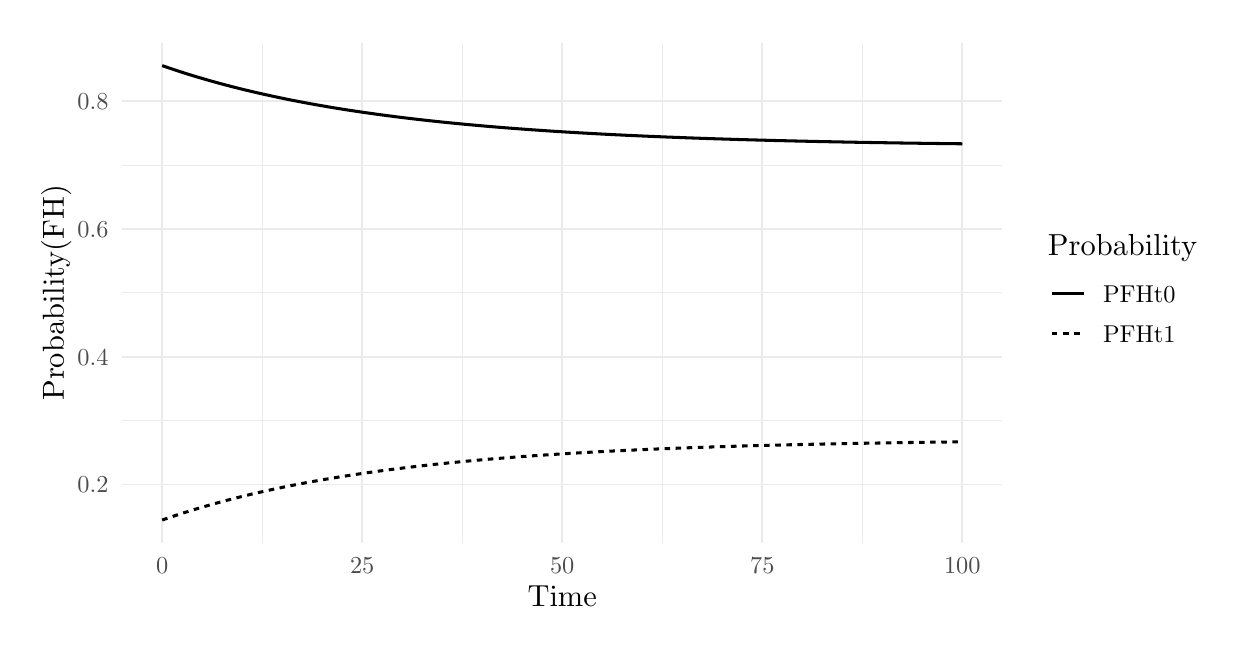
\begin{tikzpicture}[x=1pt,y=1pt, scale=1]
\definecolor{fillColor}{RGB}{255,255,255}
\path[use as bounding box,fill=fillColor,fill opacity=0.00] (0,0) rectangle (433.62,216.81);
\begin{scope}
\path[clip] ( 34.16, 30.69) rectangle (352.17,211.31);
\definecolor{drawColor}{gray}{0.92}

\path[draw=drawColor,line width= 0.3pt,line join=round] ( 34.16, 74.85) --
	(352.17, 74.85);

\path[draw=drawColor,line width= 0.3pt,line join=round] ( 34.16,121.00) --
	(352.17,121.00);

\path[draw=drawColor,line width= 0.3pt,line join=round] ( 34.16,167.15) --
	(352.17,167.15);

\path[draw=drawColor,line width= 0.3pt,line join=round] ( 84.75, 30.69) --
	( 84.75,211.31);

\path[draw=drawColor,line width= 0.3pt,line join=round] (157.03, 30.69) --
	(157.03,211.31);

\path[draw=drawColor,line width= 0.3pt,line join=round] (229.30, 30.69) --
	(229.30,211.31);

\path[draw=drawColor,line width= 0.3pt,line join=round] (301.58, 30.69) --
	(301.58,211.31);

\path[draw=drawColor,line width= 0.6pt,line join=round] ( 34.16, 51.77) --
	(352.17, 51.77);

\path[draw=drawColor,line width= 0.6pt,line join=round] ( 34.16, 97.92) --
	(352.17, 97.92);

\path[draw=drawColor,line width= 0.6pt,line join=round] ( 34.16,144.07) --
	(352.17,144.07);

\path[draw=drawColor,line width= 0.6pt,line join=round] ( 34.16,190.23) --
	(352.17,190.23);

\path[draw=drawColor,line width= 0.6pt,line join=round] ( 48.61, 30.69) --
	( 48.61,211.31);

\path[draw=drawColor,line width= 0.6pt,line join=round] (120.89, 30.69) --
	(120.89,211.31);

\path[draw=drawColor,line width= 0.6pt,line join=round] (193.16, 30.69) --
	(193.16,211.31);

\path[draw=drawColor,line width= 0.6pt,line join=round] (265.44, 30.69) --
	(265.44,211.31);

\path[draw=drawColor,line width= 0.6pt,line join=round] (337.72, 30.69) --
	(337.72,211.31);
\definecolor{drawColor}{RGB}{0,0,0}

\path[draw=drawColor,line width= 1.1pt,line join=round] ( 48.61,203.10) --
	( 51.50,202.10) --
	( 54.39,201.14) --
	( 57.28,200.21) --
	( 60.18,199.32) --
	( 63.07,198.46) --
	( 65.96,197.62) --
	( 68.85,196.82) --
	( 71.74,196.04) --
	( 74.63,195.29) --
	( 77.52,194.57) --
	( 80.41,193.87) --
	( 83.30,193.20) --
	( 86.20,192.55) --
	( 89.09,191.92) --
	( 91.98,191.31) --
	( 94.87,190.72) --
	( 97.76,190.16) --
	(100.65,189.61) --
	(103.54,189.08) --
	(106.43,188.57) --
	(109.32,188.08) --
	(112.21,187.60) --
	(115.11,187.14) --
	(118.00,186.70) --
	(120.89,186.27) --
	(123.78,185.86) --
	(126.67,185.46) --
	(129.56,185.07) --
	(132.45,184.70) --
	(135.34,184.33) --
	(138.23,183.99) --
	(141.13,183.65) --
	(144.02,183.32) --
	(146.91,183.01) --
	(149.80,182.70) --
	(152.69,182.41) --
	(155.58,182.13) --
	(158.47,181.85) --
	(161.36,181.59) --
	(164.25,181.33) --
	(167.14,181.08) --
	(170.04,180.84) --
	(172.93,180.61) --
	(175.82,180.39) --
	(178.71,180.17) --
	(181.60,179.96) --
	(184.49,179.76) --
	(187.38,179.56) --
	(190.27,179.37) --
	(193.16,179.19) --
	(196.05,179.01) --
	(198.95,178.84) --
	(201.84,178.68) --
	(204.73,178.52) --
	(207.62,178.36) --
	(210.51,178.21) --
	(213.40,178.07) --
	(216.29,177.93) --
	(219.18,177.80) --
	(222.07,177.67) --
	(224.97,177.54) --
	(227.86,177.42) --
	(230.75,177.30) --
	(233.64,177.19) --
	(236.53,177.08) --
	(239.42,176.97) --
	(242.31,176.87) --
	(245.20,176.77) --
	(248.09,176.67) --
	(250.98,176.58) --
	(253.88,176.49) --
	(256.77,176.40) --
	(259.66,176.32) --
	(262.55,176.24) --
	(265.44,176.16) --
	(268.33,176.08) --
	(271.22,176.01) --
	(274.11,175.94) --
	(277.00,175.87) --
	(279.90,175.80) --
	(282.79,175.74) --
	(285.68,175.67) --
	(288.57,175.61) --
	(291.46,175.56) --
	(294.35,175.50) --
	(297.24,175.44) --
	(300.13,175.39) --
	(303.02,175.34) --
	(305.91,175.29) --
	(308.81,175.24) --
	(311.70,175.20) --
	(314.59,175.15) --
	(317.48,175.11) --
	(320.37,175.07) --
	(323.26,175.03) --
	(326.15,174.99) --
	(329.04,174.95) --
	(331.93,174.92) --
	(334.83,174.88) --
	(337.72,174.85);

\path[draw=drawColor,line width= 1.1pt,dash pattern=on 2pt off 2pt ,line join=round] ( 48.61, 38.90) --
	( 51.50, 39.89) --
	( 54.39, 40.85) --
	( 57.28, 41.78) --
	( 60.18, 42.68) --
	( 63.07, 43.54) --
	( 65.96, 44.37) --
	( 68.85, 45.18) --
	( 71.74, 45.95) --
	( 74.63, 46.70) --
	( 77.52, 47.43) --
	( 80.41, 48.13) --
	( 83.30, 48.80) --
	( 86.20, 49.45) --
	( 89.09, 50.08) --
	( 91.98, 50.69) --
	( 94.87, 51.27) --
	( 97.76, 51.84) --
	(100.65, 52.39) --
	(103.54, 52.91) --
	(106.43, 53.42) --
	(109.32, 53.92) --
	(112.21, 54.39) --
	(115.11, 54.85) --
	(118.00, 55.30) --
	(120.89, 55.72) --
	(123.78, 56.14) --
	(126.67, 56.54) --
	(129.56, 56.93) --
	(132.45, 57.30) --
	(135.34, 57.66) --
	(138.23, 58.01) --
	(141.13, 58.35) --
	(144.02, 58.67) --
	(146.91, 58.99) --
	(149.80, 59.29) --
	(152.69, 59.59) --
	(155.58, 59.87) --
	(158.47, 60.15) --
	(161.36, 60.41) --
	(164.25, 60.67) --
	(167.14, 60.92) --
	(170.04, 61.15) --
	(172.93, 61.39) --
	(175.82, 61.61) --
	(178.71, 61.83) --
	(181.60, 62.04) --
	(184.49, 62.24) --
	(187.38, 62.43) --
	(190.27, 62.62) --
	(193.16, 62.81) --
	(196.05, 62.98) --
	(198.95, 63.15) --
	(201.84, 63.32) --
	(204.73, 63.48) --
	(207.62, 63.63) --
	(210.51, 63.78) --
	(213.40, 63.93) --
	(216.29, 64.06) --
	(219.18, 64.20) --
	(222.07, 64.33) --
	(224.97, 64.46) --
	(227.86, 64.58) --
	(230.75, 64.70) --
	(233.64, 64.81) --
	(236.53, 64.92) --
	(239.42, 65.03) --
	(242.31, 65.13) --
	(245.20, 65.23) --
	(248.09, 65.32) --
	(250.98, 65.42) --
	(253.88, 65.51) --
	(256.77, 65.60) --
	(259.66, 65.68) --
	(262.55, 65.76) --
	(265.44, 65.84) --
	(268.33, 65.92) --
	(271.22, 65.99) --
	(274.11, 66.06) --
	(277.00, 66.13) --
	(279.90, 66.20) --
	(282.79, 66.26) --
	(285.68, 66.32) --
	(288.57, 66.38) --
	(291.46, 66.44) --
	(294.35, 66.50) --
	(297.24, 66.55) --
	(300.13, 66.60) --
	(303.02, 66.65) --
	(305.91, 66.70) --
	(308.81, 66.75) --
	(311.70, 66.80) --
	(314.59, 66.84) --
	(317.48, 66.89) --
	(320.37, 66.93) --
	(323.26, 66.97) --
	(326.15, 67.01) --
	(329.04, 67.04) --
	(331.93, 67.08) --
	(334.83, 67.12) --
	(337.72, 67.15);
\end{scope}
\begin{scope}
\path[clip] (  0.00,  0.00) rectangle (433.62,216.81);
\definecolor{drawColor}{gray}{0.30}

\node[text=drawColor,anchor=base east,inner sep=0pt, outer sep=0pt, scale=  0.88] at ( 29.21, 48.74) {0.2};

\node[text=drawColor,anchor=base east,inner sep=0pt, outer sep=0pt, scale=  0.88] at ( 29.21, 94.89) {0.4};

\node[text=drawColor,anchor=base east,inner sep=0pt, outer sep=0pt, scale=  0.88] at ( 29.21,141.04) {0.6};

\node[text=drawColor,anchor=base east,inner sep=0pt, outer sep=0pt, scale=  0.88] at ( 29.21,187.20) {0.8};
\end{scope}
\begin{scope}
\path[clip] (  0.00,  0.00) rectangle (433.62,216.81);
\definecolor{drawColor}{gray}{0.30}

\node[text=drawColor,anchor=base,inner sep=0pt, outer sep=0pt, scale=  0.88] at ( 48.61, 19.68) {0};

\node[text=drawColor,anchor=base,inner sep=0pt, outer sep=0pt, scale=  0.88] at (120.89, 19.68) {25};

\node[text=drawColor,anchor=base,inner sep=0pt, outer sep=0pt, scale=  0.88] at (193.16, 19.68) {50};

\node[text=drawColor,anchor=base,inner sep=0pt, outer sep=0pt, scale=  0.88] at (265.44, 19.68) {75};

\node[text=drawColor,anchor=base,inner sep=0pt, outer sep=0pt, scale=  0.88] at (337.72, 19.68) {100};
\end{scope}
\begin{scope}
\path[clip] (  0.00,  0.00) rectangle (433.62,216.81);
\definecolor{drawColor}{RGB}{0,0,0}

\node[text=drawColor,anchor=base,inner sep=0pt, outer sep=0pt, scale=  1.10] at (193.16,  7.64) {Time};
\end{scope}
\begin{scope}
\path[clip] (  0.00,  0.00) rectangle (433.62,216.81);
\definecolor{drawColor}{RGB}{0,0,0}

\node[text=drawColor,rotate= 90.00,anchor=base,inner sep=0pt, outer sep=0pt, scale=  1.10] at ( 13.08,121.00) {Probability(FH)};
\end{scope}
\begin{scope}
\path[clip] (  0.00,  0.00) rectangle (433.62,216.81);
\definecolor{drawColor}{RGB}{0,0,0}

\node[text=drawColor,anchor=base west,inner sep=0pt, outer sep=0pt, scale=  1.10] at (368.67,134.41) {Probability};
\end{scope}
\begin{scope}
\path[clip] (  0.00,  0.00) rectangle (433.62,216.81);
\definecolor{drawColor}{RGB}{0,0,0}

\path[draw=drawColor,line width= 1.1pt,line join=round] (370.12,120.62) -- (381.68,120.62);
\end{scope}
\begin{scope}
\path[clip] (  0.00,  0.00) rectangle (433.62,216.81);
\definecolor{drawColor}{RGB}{0,0,0}

\path[draw=drawColor,line width= 1.1pt,dash pattern=on 2pt off 2pt ,line join=round] (370.12,106.16) -- (381.68,106.16);
\end{scope}
\begin{scope}
\path[clip] (  0.00,  0.00) rectangle (433.62,216.81);
\definecolor{drawColor}{RGB}{0,0,0}

\node[text=drawColor,anchor=base west,inner sep=0pt, outer sep=0pt, scale=  0.88] at (388.63,117.59) {PFHt0};
\end{scope}
\begin{scope}
\path[clip] (  0.00,  0.00) rectangle (433.62,216.81);
\definecolor{drawColor}{RGB}{0,0,0}

\node[text=drawColor,anchor=base west,inner sep=0pt, outer sep=0pt, scale=  0.88] at (388.63,103.13) {PFHt1};
\end{scope}
\end{tikzpicture}
    \caption{probability of FH = 0 (PFHt0) vs Probability of FH = 1 (PFHt1).}
    \label{fig:disease 0}
\end{figure}
The difference between the two indicators can assume the values: $(FH(t) - R) \in \left\{-1, 0, 1\right\}$. We would like to be as close as possible to the scenario with no difference between the indicators. Importantly, $R$ is fixed while $FH(t)$ depends on $t$. 

% We compute the probabilities of the agreement for low and high-risk group membership. The conditional probability of agreement in the low-risk group over the whole $\mathbb{R}^+$ time axis is:

We now compute the probabilities of the agreement for low-risk group and high-risk group membership. For the survival case we recall that the hazard function in the low (high) risk group is $\lambda_0(t)$ ($\lambda_1(t)=\alpha\cdot\lambda_0(t)$), keeping in mind that  $\lambda(t\mid R=0)=\lambda_0=\lambda$ and $\lambda(t\mid R=1)=\lambda_1(t)=\beta\lambda_0(t)=\beta\lambda$. But this does not hold in the disease development case. The probability of agreement in the low-risk group over the whole $\mathbb{R}^+$ time axis is: 
\begin{align*}
    %\label{prob_0}
    &P(FH (b +t) = R \mid R =0) =\int_0^{\infty}P(FH (b +t)=0)f_{0}(t)\text{d}t \nonumber \\
    &=\int_0^{\infty}\left(p+(1-p)\text{e}^{-\lambda(t+60)}\right)\left(p+(1-p)\text{e}^{-\lambda^*(t+30)}\right)
    \left(p+(1-p)\text{e}^{-\lambda^*t}\right)(1-p)\lambda \text{e}^{-\lambda t}\text{d}t.
\end{align*}
Similarly, we compute the probability of agreement for the high-risk group:
    \begin{align*}
    %\label{prob_1}
    &P(FH (b +t) = R \mid R =1) =\int_0^{\infty}P(FH (b +t)=1)f_{1}(t)\text{d}t \\
    &=\int_0^{\infty}(1 - P(FH (b +t)=0))f_1(t,\lambda )\text{d}t =\int_0^{\infty}f_1(t,\lambda ) - P(FH (b +t)=0)f_1(t,\lambda )\text{d}t \nonumber \\
    &=\int_0^{\infty}f_1(t,\lambda )\text{d}t - \int_0^{\infty}P(FH (b +t)=0)f_1(t,\lambda )\text{d}t =1 - \int_0^{\infty}P(FH (b +t)=0)f_1(t,\lambda )\text{d}t\nonumber \\
    &=1 - \int_0^{\infty}P(FH (b +t)=0)(1-\widetilde{p})\left(\dfrac{\widetilde f(t)\alpha}{1-\widetilde{p}}\right)(p+(1-p)\widetilde S(t))^{\alpha-1}\text{d}t. \nonumber
\end{align*} 

One would like both probabilities to be large. For the cure rate case, the conditional probability of agreement in the low-risk group over the whole $\mathbb{R}^+$ time axis is
\begin{align*}
    % \label{formula:1_2}
    P(FH (b +t) = R \mid R =0) &=\int_0^{\infty}P(FH (b +t)=0)f_0(t)\text{d}t.
\end{align*} 

Easily, we obtain the conditional probability of agreement for the high-risk group, such as 
\begin{align*}
    % \label{formula:1_3}
    P(F H (b +t) = R \mid R =1)  &=\int_0^{\infty}P(F H (b +t)=1)f_1(t)\text{d}t
\end{align*} 

We can also analyse the misclassification probabilities (notice that we implicitly assume that the proportion of high-risk families $P(R=1)=h$ is constant over time).
For the cure rate case the conditional correct classification probabilities are \begin{align*}
    % \label{probs_final}
    &P(FH (t)=0\mid R =0)=S_0(t+60)S_0(t+30)S_0(t) \\
    &=(p+(1-p)\widetilde S(t+60)) (p+(1-p)\widetilde S(t+30)) (p+(1-p)\widetilde S(t)) \\
    &=(p+(1-p)e^{-\lambda(t+60)}) (p+(1-p)e^{-\lambda(t+30)}) (p+(1-p)e^{-\lambda(t)}) \\
    &P(FH (t)=0\mid R =1) = S_1(t+60)S_1(t+30)S_1(t) =(S_0(t+60)S_0(t+30)S_0(t))^{\alpha} \\
    &=((p+(1-p)e^{-\lambda(t+60)}) (p+(1-p)e^{-\lambda(t+30)}) (p+(1-p)e^{-\lambda(t)}))^\alpha
\end{align*} 

Clearly, \begin{align*}
    &P(FH (t)=1\mid R =0) = 1 - S_0(t+60)S_0(t+30)S_0(t) \\
    &P(FH (t)=1\mid R =1) = 1 - S_1(t+60)S_1(t+30)S_1(t)
\end{align*} 
where $S_0(t) = p+(1-p)e^{-\lambda(t)}$, and $S_1(t) = (p+(1-p)e^{-\lambda(t)})^\alpha$. 

A graphical visualization of these probabilities is illustrated in Figure \ref{fig:disease 1}. 
\begin{figure}[ht]
    \centering
    % \includegraphics{plots/plot_1_disease.png}
    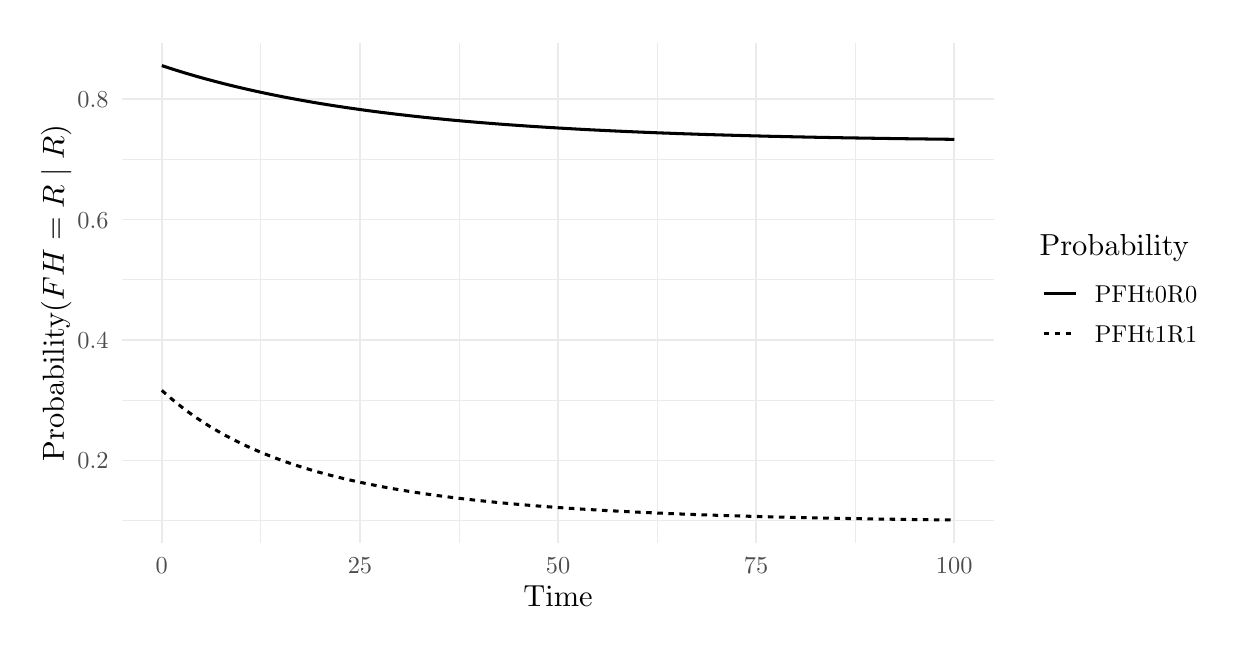
\begin{tikzpicture}[x=1pt,y=1pt,scale=1]
\definecolor{fillColor}{RGB}{255,255,255}
\path[use as bounding box,fill=fillColor,fill opacity=0.00] (0,0) rectangle (433.62,216.81);
\begin{scope}
\path[clip] ( 34.16, 30.69) rectangle (349.14,211.31);
\definecolor{drawColor}{gray}{0.92}

\path[draw=drawColor,line width= 0.3pt,line join=round] ( 34.16, 38.66) --
	(349.14, 38.66);

\path[draw=drawColor,line width= 0.3pt,line join=round] ( 34.16, 82.17) --
	(349.14, 82.17);

\path[draw=drawColor,line width= 0.3pt,line join=round] ( 34.16,125.69) --
	(349.14,125.69);

\path[draw=drawColor,line width= 0.3pt,line join=round] ( 34.16,169.20) --
	(349.14,169.20);

\path[draw=drawColor,line width= 0.3pt,line join=round] ( 84.27, 30.69) --
	( 84.27,211.31);

\path[draw=drawColor,line width= 0.3pt,line join=round] (155.86, 30.69) --
	(155.86,211.31);

\path[draw=drawColor,line width= 0.3pt,line join=round] (227.44, 30.69) --
	(227.44,211.31);

\path[draw=drawColor,line width= 0.3pt,line join=round] (299.03, 30.69) --
	(299.03,211.31);

\path[draw=drawColor,line width= 0.6pt,line join=round] ( 34.16, 60.41) --
	(349.14, 60.41);

\path[draw=drawColor,line width= 0.6pt,line join=round] ( 34.16,103.93) --
	(349.14,103.93);

\path[draw=drawColor,line width= 0.6pt,line join=round] ( 34.16,147.45) --
	(349.14,147.45);

\path[draw=drawColor,line width= 0.6pt,line join=round] ( 34.16,190.96) --
	(349.14,190.96);

\path[draw=drawColor,line width= 0.6pt,line join=round] ( 48.47, 30.69) --
	( 48.47,211.31);

\path[draw=drawColor,line width= 0.6pt,line join=round] (120.06, 30.69) --
	(120.06,211.31);

\path[draw=drawColor,line width= 0.6pt,line join=round] (191.65, 30.69) --
	(191.65,211.31);

\path[draw=drawColor,line width= 0.6pt,line join=round] (263.24, 30.69) --
	(263.24,211.31);

\path[draw=drawColor,line width= 0.6pt,line join=round] (334.82, 30.69) --
	(334.82,211.31);
\definecolor{drawColor}{RGB}{0,0,0}

\path[draw=drawColor,line width= 1.1pt,line join=round] ( 48.47,203.10) --
	( 51.34,202.16) --
	( 54.20,201.25) --
	( 57.06,200.38) --
	( 59.93,199.54) --
	( 62.79,198.72) --
	( 65.65,197.94) --
	( 68.52,197.18) --
	( 71.38,196.45) --
	( 74.25,195.74) --
	( 77.11,195.06) --
	( 79.97,194.40) --
	( 82.84,193.76) --
	( 85.70,193.15) --
	( 88.56,192.56) --
	( 91.43,191.98) --
	( 94.29,191.43) --
	( 97.15,190.90) --
	(100.02,190.38) --
	(102.88,189.88) --
	(105.74,189.40) --
	(108.61,188.94) --
	(111.47,188.49) --
	(114.33,188.06) --
	(117.20,187.64) --
	(120.06,187.23) --
	(122.92,186.84) --
	(125.79,186.46) --
	(128.65,186.10) --
	(131.52,185.75) --
	(134.38,185.41) --
	(137.24,185.08) --
	(140.11,184.76) --
	(142.97,184.45) --
	(145.83,184.16) --
	(148.70,183.87) --
	(151.56,183.59) --
	(154.42,183.32) --
	(157.29,183.06) --
	(160.15,182.81) --
	(163.01,182.57) --
	(165.88,182.34) --
	(168.74,182.11) --
	(171.60,181.89) --
	(174.47,181.68) --
	(177.33,181.48) --
	(180.19,181.28) --
	(183.06,181.09) --
	(185.92,180.91) --
	(188.79,180.73) --
	(191.65,180.56) --
	(194.51,180.39) --
	(197.38,180.23) --
	(200.24,180.07) --
	(203.10,179.92) --
	(205.97,179.78) --
	(208.83,179.64) --
	(211.69,179.50) --
	(214.56,179.37) --
	(217.42,179.24) --
	(220.28,179.12) --
	(223.15,179.00) --
	(226.01,178.88) --
	(228.87,178.77) --
	(231.74,178.67) --
	(234.60,178.56) --
	(237.46,178.46) --
	(240.33,178.37) --
	(243.19,178.27) --
	(246.06,178.18) --
	(248.92,178.09) --
	(251.78,178.01) --
	(254.65,177.93) --
	(257.51,177.85) --
	(260.37,177.77) --
	(263.24,177.70) --
	(266.10,177.62) --
	(268.96,177.55) --
	(271.83,177.49) --
	(274.69,177.42) --
	(277.55,177.36) --
	(280.42,177.30) --
	(283.28,177.24) --
	(286.14,177.18) --
	(289.01,177.13) --
	(291.87,177.08) --
	(294.73,177.02) --
	(297.60,176.97) --
	(300.46,176.93) --
	(303.33,176.88) --
	(306.19,176.84) --
	(309.05,176.79) --
	(311.92,176.75) --
	(314.78,176.71) --
	(317.64,176.67) --
	(320.51,176.63) --
	(323.37,176.60) --
	(326.23,176.56) --
	(329.10,176.53) --
	(331.96,176.49) --
	(334.82,176.46);

\path[draw=drawColor,line width= 1.1pt,dash pattern=on 2pt off 2pt ,line join=round] ( 48.47, 85.74) --
	( 51.34, 83.22) --
	( 54.20, 80.86) --
	( 57.06, 78.65) --
	( 59.93, 76.58) --
	( 62.79, 74.64) --
	( 65.65, 72.82) --
	( 68.52, 71.11) --
	( 71.38, 69.51) --
	( 74.25, 68.00) --
	( 77.11, 66.57) --
	( 79.97, 65.23) --
	( 82.84, 63.97) --
	( 85.70, 62.78) --
	( 88.56, 61.65) --
	( 91.43, 60.58) --
	( 94.29, 59.57) --
	( 97.15, 58.62) --
	(100.02, 57.71) --
	(102.88, 56.85) --
	(105.74, 56.04) --
	(108.61, 55.27) --
	(111.47, 54.54) --
	(114.33, 53.84) --
	(117.20, 53.18) --
	(120.06, 52.55) --
	(122.92, 51.95) --
	(125.79, 51.38) --
	(128.65, 50.83) --
	(131.52, 50.31) --
	(134.38, 49.82) --
	(137.24, 49.35) --
	(140.11, 48.90) --
	(142.97, 48.46) --
	(145.83, 48.05) --
	(148.70, 47.66) --
	(151.56, 47.29) --
	(154.42, 46.93) --
	(157.29, 46.58) --
	(160.15, 46.25) --
	(163.01, 45.94) --
	(165.88, 45.64) --
	(168.74, 45.35) --
	(171.60, 45.07) --
	(174.47, 44.81) --
	(177.33, 44.55) --
	(180.19, 44.31) --
	(183.06, 44.07) --
	(185.92, 43.85) --
	(188.79, 43.63) --
	(191.65, 43.43) --
	(194.51, 43.23) --
	(197.38, 43.04) --
	(200.24, 42.85) --
	(203.10, 42.68) --
	(205.97, 42.51) --
	(208.83, 42.34) --
	(211.69, 42.19) --
	(214.56, 42.04) --
	(217.42, 41.89) --
	(220.28, 41.75) --
	(223.15, 41.62) --
	(226.01, 41.49) --
	(228.87, 41.37) --
	(231.74, 41.25) --
	(234.60, 41.13) --
	(237.46, 41.02) --
	(240.33, 40.91) --
	(243.19, 40.81) --
	(246.06, 40.71) --
	(248.92, 40.61) --
	(251.78, 40.52) --
	(254.65, 40.43) --
	(257.51, 40.35) --
	(260.37, 40.27) --
	(263.24, 40.19) --
	(266.10, 40.11) --
	(268.96, 40.04) --
	(271.83, 39.96) --
	(274.69, 39.90) --
	(277.55, 39.83) --
	(280.42, 39.77) --
	(283.28, 39.70) --
	(286.14, 39.64) --
	(289.01, 39.59) --
	(291.87, 39.53) --
	(294.73, 39.48) --
	(297.60, 39.43) --
	(300.46, 39.38) --
	(303.33, 39.33) --
	(306.19, 39.28) --
	(309.05, 39.24) --
	(311.92, 39.19) --
	(314.78, 39.15) --
	(317.64, 39.11) --
	(320.51, 39.07) --
	(323.37, 39.03) --
	(326.23, 39.00) --
	(329.10, 38.96) --
	(331.96, 38.93) --
	(334.82, 38.90);
\end{scope}
\begin{scope}
\path[clip] (  0.00,  0.00) rectangle (433.62,216.81);
\definecolor{drawColor}{gray}{0.30}

\node[text=drawColor,anchor=base east,inner sep=0pt, outer sep=0pt, scale=  0.88] at ( 29.21, 57.38) {0.2};

\node[text=drawColor,anchor=base east,inner sep=0pt, outer sep=0pt, scale=  0.88] at ( 29.21,100.90) {0.4};

\node[text=drawColor,anchor=base east,inner sep=0pt, outer sep=0pt, scale=  0.88] at ( 29.21,144.42) {0.6};

\node[text=drawColor,anchor=base east,inner sep=0pt, outer sep=0pt, scale=  0.88] at ( 29.21,187.93) {0.8};
\end{scope}
\begin{scope}
\path[clip] (  0.00,  0.00) rectangle (433.62,216.81);
\definecolor{drawColor}{gray}{0.30}

\node[text=drawColor,anchor=base,inner sep=0pt, outer sep=0pt, scale=  0.88] at ( 48.47, 19.68) {0};

\node[text=drawColor,anchor=base,inner sep=0pt, outer sep=0pt, scale=  0.88] at (120.06, 19.68) {25};

\node[text=drawColor,anchor=base,inner sep=0pt, outer sep=0pt, scale=  0.88] at (191.65, 19.68) {50};

\node[text=drawColor,anchor=base,inner sep=0pt, outer sep=0pt, scale=  0.88] at (263.24, 19.68) {75};

\node[text=drawColor,anchor=base,inner sep=0pt, outer sep=0pt, scale=  0.88] at (334.82, 19.68) {100};
\end{scope}
\begin{scope}
\path[clip] (  0.00,  0.00) rectangle (433.62,216.81);
\definecolor{drawColor}{RGB}{0,0,0}

\node[text=drawColor,anchor=base,inner sep=0pt, outer sep=0pt, scale=  1.10] at (191.65,  7.64) {Time};
\end{scope}
\begin{scope}
\path[clip] (  0.00,  0.00) rectangle (433.62,216.81);
\definecolor{drawColor}{RGB}{0,0,0}

\node[text=drawColor,rotate= 90.00,anchor=base,inner sep=0pt, outer sep=0pt, scale=  1.10] at ( 13.08,121.00) {Probability($FH = R\mid R$)};
\end{scope}
\begin{scope}
\path[clip] (  0.00,  0.00) rectangle (433.62,216.81);
\definecolor{drawColor}{RGB}{0,0,0}

\node[text=drawColor,anchor=base west,inner sep=0pt, outer sep=0pt, scale=  1.10] at (365.64,134.41) {Probability};
\end{scope}
\begin{scope}
\path[clip] (  0.00,  0.00) rectangle (433.62,216.81);
\definecolor{drawColor}{RGB}{0,0,0}

\path[draw=drawColor,line width= 1.1pt,line join=round] (367.09,120.62) -- (378.65,120.62);
\end{scope}
\begin{scope}
\path[clip] (  0.00,  0.00) rectangle (433.62,216.81);
\definecolor{drawColor}{RGB}{0,0,0}

\path[draw=drawColor,line width= 1.1pt,dash pattern=on 2pt off 2pt ,line join=round] (367.09,106.16) -- (378.65,106.16);
\end{scope}
\begin{scope}
\path[clip] (  0.00,  0.00) rectangle (433.62,216.81);
\definecolor{drawColor}{RGB}{0,0,0}

\node[text=drawColor,anchor=base west,inner sep=0pt, outer sep=0pt, scale=  0.88] at (385.60,117.59) {PFHt0R0};
\end{scope}
\begin{scope}
\path[clip] (  0.00,  0.00) rectangle (433.62,216.81);
\definecolor{drawColor}{RGB}{0,0,0}

\node[text=drawColor,anchor=base west,inner sep=0pt, outer sep=0pt, scale=  0.88] at (385.60,103.13) {PFHt1R1};
\end{scope}
\end{tikzpicture}
    \caption{probability of $FH = 0$ conditional to $R = 0$ (PFHt0R0) vs. Probability of $(FH = 1$ conditional to $R=1$ (PFHt1R1).}
    \label{fig:disease 1}
\end{figure}
We also compute the inverse probabilities of correct classification only for the survival case, i.e.: (i) $P(R =0\mid FH (t)=0)$ and (ii) $P(R =1\mid FH (t)=1)$. These are: \begin{align*}
    &(i) \ P(R  = 0\mid FH (t)=0) = \dfrac{P(FH (t)=0\mid R =0)P(R =0)}{P(FH (t)=0)} \\
    &= \dfrac{P(FH (t)=0\mid R =0)(1-h)}{P(FH (t)=0\mid R =0)(1-h) +P(FH (t)=0\mid R =1)h} = \dfrac{f(t,p,\lambda )(1-h)}{f(t,p,\lambda )(1-h)+\left(f(t,p,\lambda )^{\alpha} \right)h}
\end{align*} and \begin{align*}
    &(ii) \ P(R  = 1\mid FH (t)=1) = \dfrac{P(FH (t)=1\mid R =1)P(R =1)}{P(FH (t)=1)}  \\
    &= \dfrac{P(FH (t)=1\mid R =1)h}{P(FH (t)=1\mid R =1)h +P(FH (t)=1\mid R =0)(1-h) } \\
    &=\dfrac{(1-f(t,p,\lambda )^{\alpha})h}{(1-f(t,p,\lambda )^{\alpha})h+\left(1-f(t,p,\lambda )\right)(1-h)}
\end{align*}
with $f(t,p,\lambda ) = (p+(1-p)e^{-\lambda (t+60)}) (p+(1-p)e^{-\lambda (t+30)}) (p+(1-p)e^{-\lambda (t)})$.
With these probabilities, we describe the distribution of the measurement error when using the observed $FH(t)$ instead of $R$ in the observed data model. A graphical representation of the trend of these probabilities for the fixed values $\lambda=1/90$, $\alpha=2$, $h=0.7$ is illustrated in Figure \ref{fig:disease 2}. \begin{figure}[ht]
    \centering
    % \includegraphics{plots/plot_2_disease.png}
    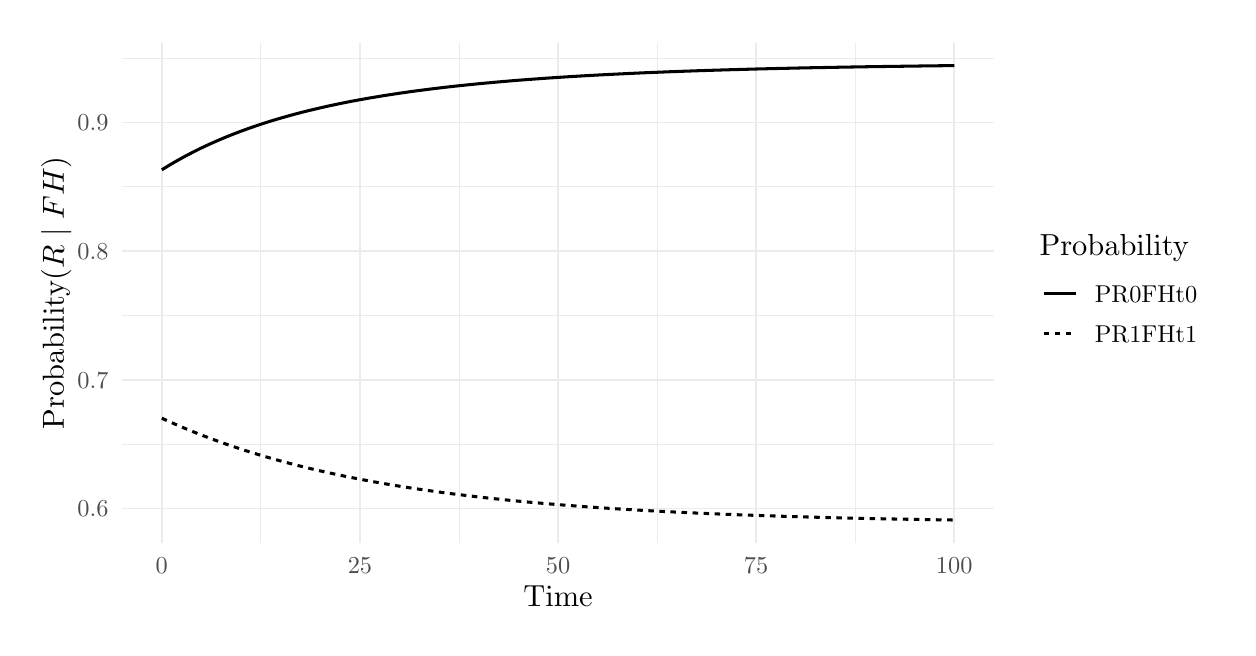
\begin{tikzpicture}[x=1pt,y=1pt,scale=1]
\definecolor{fillColor}{RGB}{255,255,255}
\path[use as bounding box,fill=fillColor,fill opacity=0.00] (0,0) rectangle (433.62,216.81);
\begin{scope}
\path[clip] ( 34.16, 30.69) rectangle (349.14,211.31);
\definecolor{drawColor}{gray}{0.92}

\path[draw=drawColor,line width= 0.3pt,line join=round] ( 34.16, 66.34) --
	(349.14, 66.34);

\path[draw=drawColor,line width= 0.3pt,line join=round] ( 34.16,112.82) --
	(349.14,112.82);

\path[draw=drawColor,line width= 0.3pt,line join=round] ( 34.16,159.31) --
	(349.14,159.31);

\path[draw=drawColor,line width= 0.3pt,line join=round] ( 34.16,205.79) --
	(349.14,205.79);

\path[draw=drawColor,line width= 0.3pt,line join=round] ( 84.27, 30.69) --
	( 84.27,211.31);

\path[draw=drawColor,line width= 0.3pt,line join=round] (155.86, 30.69) --
	(155.86,211.31);

\path[draw=drawColor,line width= 0.3pt,line join=round] (227.44, 30.69) --
	(227.44,211.31);

\path[draw=drawColor,line width= 0.3pt,line join=round] (299.03, 30.69) --
	(299.03,211.31);

\path[draw=drawColor,line width= 0.6pt,line join=round] ( 34.16, 43.10) --
	(349.14, 43.10);

\path[draw=drawColor,line width= 0.6pt,line join=round] ( 34.16, 89.58) --
	(349.14, 89.58);

\path[draw=drawColor,line width= 0.6pt,line join=round] ( 34.16,136.07) --
	(349.14,136.07);

\path[draw=drawColor,line width= 0.6pt,line join=round] ( 34.16,182.55) --
	(349.14,182.55);

\path[draw=drawColor,line width= 0.6pt,line join=round] ( 48.47, 30.69) --
	( 48.47,211.31);

\path[draw=drawColor,line width= 0.6pt,line join=round] (120.06, 30.69) --
	(120.06,211.31);

\path[draw=drawColor,line width= 0.6pt,line join=round] (191.65, 30.69) --
	(191.65,211.31);

\path[draw=drawColor,line width= 0.6pt,line join=round] (263.24, 30.69) --
	(263.24,211.31);

\path[draw=drawColor,line width= 0.6pt,line join=round] (334.82, 30.69) --
	(334.82,211.31);
\definecolor{drawColor}{RGB}{0,0,0}

\path[draw=drawColor,line width= 1.1pt,line join=round] ( 48.47,165.45) --
	( 51.34,167.21) --
	( 54.20,168.87) --
	( 57.06,170.44) --
	( 59.93,171.93) --
	( 62.79,173.35) --
	( 65.65,174.69) --
	( 68.52,175.96) --
	( 71.38,177.17) --
	( 74.25,178.32) --
	( 77.11,179.41) --
	( 79.97,180.45) --
	( 82.84,181.44) --
	( 85.70,182.38) --
	( 88.56,183.28) --
	( 91.43,184.13) --
	( 94.29,184.94) --
	( 97.15,185.72) --
	(100.02,186.46) --
	(102.88,187.16) --
	(105.74,187.83) --
	(108.61,188.48) --
	(111.47,189.09) --
	(114.33,189.68) --
	(117.20,190.24) --
	(120.06,190.77) --
	(122.92,191.28) --
	(125.79,191.77) --
	(128.65,192.24) --
	(131.52,192.69) --
	(134.38,193.12) --
	(137.24,193.53) --
	(140.11,193.93) --
	(142.97,194.30) --
	(145.83,194.67) --
	(148.70,195.01) --
	(151.56,195.35) --
	(154.42,195.67) --
	(157.29,195.97) --
	(160.15,196.27) --
	(163.01,196.55) --
	(165.88,196.82) --
	(168.74,197.08) --
	(171.60,197.33) --
	(174.47,197.58) --
	(177.33,197.81) --
	(180.19,198.03) --
	(183.06,198.24) --
	(185.92,198.45) --
	(188.79,198.65) --
	(191.65,198.84) --
	(194.51,199.02) --
	(197.38,199.20) --
	(200.24,199.37) --
	(203.10,199.53) --
	(205.97,199.69) --
	(208.83,199.84) --
	(211.69,199.98) --
	(214.56,200.12) --
	(217.42,200.26) --
	(220.28,200.39) --
	(223.15,200.52) --
	(226.01,200.64) --
	(228.87,200.75) --
	(231.74,200.87) --
	(234.60,200.97) --
	(237.46,201.08) --
	(240.33,201.18) --
	(243.19,201.28) --
	(246.06,201.37) --
	(248.92,201.46) --
	(251.78,201.55) --
	(254.65,201.63) --
	(257.51,201.71) --
	(260.37,201.79) --
	(263.24,201.87) --
	(266.10,201.94) --
	(268.96,202.01) --
	(271.83,202.08) --
	(274.69,202.14) --
	(277.55,202.21) --
	(280.42,202.27) --
	(283.28,202.33) --
	(286.14,202.38) --
	(289.01,202.44) --
	(291.87,202.49) --
	(294.73,202.54) --
	(297.60,202.59) --
	(300.46,202.64) --
	(303.33,202.69) --
	(306.19,202.73) --
	(309.05,202.77) --
	(311.92,202.81) --
	(314.78,202.85) --
	(317.64,202.89) --
	(320.51,202.93) --
	(323.37,202.97) --
	(326.23,203.00) --
	(329.10,203.04) --
	(331.96,203.07) --
	(334.82,203.10);

\path[draw=drawColor,line width= 1.1pt,dash pattern=on 2pt off 2pt ,line join=round] ( 48.47, 75.70) --
	( 51.34, 74.39) --
	( 54.20, 73.13) --
	( 57.06, 71.92) --
	( 59.93, 70.75) --
	( 62.79, 69.61) --
	( 65.65, 68.52) --
	( 68.52, 67.46) --
	( 71.38, 66.44) --
	( 74.25, 65.46) --
	( 77.11, 64.51) --
	( 79.97, 63.59) --
	( 82.84, 62.71) --
	( 85.70, 61.85) --
	( 88.56, 61.03) --
	( 91.43, 60.23) --
	( 94.29, 59.47) --
	( 97.15, 58.72) --
	(100.02, 58.01) --
	(102.88, 57.32) --
	(105.74, 56.65) --
	(108.61, 56.01) --
	(111.47, 55.39) --
	(114.33, 54.78) --
	(117.20, 54.21) --
	(120.06, 53.65) --
	(122.92, 53.11) --
	(125.79, 52.58) --
	(128.65, 52.08) --
	(131.52, 51.59) --
	(134.38, 51.12) --
	(137.24, 50.67) --
	(140.11, 50.23) --
	(142.97, 49.81) --
	(145.83, 49.40) --
	(148.70, 49.00) --
	(151.56, 48.62) --
	(154.42, 48.25) --
	(157.29, 47.90) --
	(160.15, 47.56) --
	(163.01, 47.22) --
	(165.88, 46.90) --
	(168.74, 46.59) --
	(171.60, 46.29) --
	(174.47, 46.00) --
	(177.33, 45.72) --
	(180.19, 45.45) --
	(183.06, 45.19) --
	(185.92, 44.94) --
	(188.79, 44.70) --
	(191.65, 44.46) --
	(194.51, 44.24) --
	(197.38, 44.02) --
	(200.24, 43.80) --
	(203.10, 43.60) --
	(205.97, 43.40) --
	(208.83, 43.21) --
	(211.69, 43.02) --
	(214.56, 42.84) --
	(217.42, 42.67) --
	(220.28, 42.50) --
	(223.15, 42.34) --
	(226.01, 42.18) --
	(228.87, 42.03) --
	(231.74, 41.89) --
	(234.60, 41.75) --
	(237.46, 41.61) --
	(240.33, 41.48) --
	(243.19, 41.35) --
	(246.06, 41.23) --
	(248.92, 41.11) --
	(251.78, 40.99) --
	(254.65, 40.88) --
	(257.51, 40.77) --
	(260.37, 40.67) --
	(263.24, 40.57) --
	(266.10, 40.47) --
	(268.96, 40.38) --
	(271.83, 40.29) --
	(274.69, 40.20) --
	(277.55, 40.11) --
	(280.42, 40.03) --
	(283.28, 39.95) --
	(286.14, 39.87) --
	(289.01, 39.80) --
	(291.87, 39.73) --
	(294.73, 39.66) --
	(297.60, 39.59) --
	(300.46, 39.53) --
	(303.33, 39.46) --
	(306.19, 39.40) --
	(309.05, 39.34) --
	(311.92, 39.29) --
	(314.78, 39.23) --
	(317.64, 39.18) --
	(320.51, 39.13) --
	(323.37, 39.08) --
	(326.23, 39.03) --
	(329.10, 38.98) --
	(331.96, 38.94) --
	(334.82, 38.90);
\end{scope}
\begin{scope}
\path[clip] (  0.00,  0.00) rectangle (433.62,216.81);
\definecolor{drawColor}{gray}{0.30}

\node[text=drawColor,anchor=base east,inner sep=0pt, outer sep=0pt, scale=  0.88] at ( 29.21, 40.07) {0.6};

\node[text=drawColor,anchor=base east,inner sep=0pt, outer sep=0pt, scale=  0.88] at ( 29.21, 86.55) {0.7};

\node[text=drawColor,anchor=base east,inner sep=0pt, outer sep=0pt, scale=  0.88] at ( 29.21,133.04) {0.8};

\node[text=drawColor,anchor=base east,inner sep=0pt, outer sep=0pt, scale=  0.88] at ( 29.21,179.52) {0.9};
\end{scope}
\begin{scope}
\path[clip] (  0.00,  0.00) rectangle (433.62,216.81);
\definecolor{drawColor}{gray}{0.30}

\node[text=drawColor,anchor=base,inner sep=0pt, outer sep=0pt, scale=  0.88] at ( 48.47, 19.68) {0};

\node[text=drawColor,anchor=base,inner sep=0pt, outer sep=0pt, scale=  0.88] at (120.06, 19.68) {25};

\node[text=drawColor,anchor=base,inner sep=0pt, outer sep=0pt, scale=  0.88] at (191.65, 19.68) {50};

\node[text=drawColor,anchor=base,inner sep=0pt, outer sep=0pt, scale=  0.88] at (263.24, 19.68) {75};

\node[text=drawColor,anchor=base,inner sep=0pt, outer sep=0pt, scale=  0.88] at (334.82, 19.68) {100};
\end{scope}
\begin{scope}
\path[clip] (  0.00,  0.00) rectangle (433.62,216.81);
\definecolor{drawColor}{RGB}{0,0,0}

\node[text=drawColor,anchor=base,inner sep=0pt, outer sep=0pt, scale=  1.10] at (191.65,  7.64) {Time};
\end{scope}
\begin{scope}
\path[clip] (  0.00,  0.00) rectangle (433.62,216.81);
\definecolor{drawColor}{RGB}{0,0,0}

\node[text=drawColor,rotate= 90.00,anchor=base,inner sep=0pt, outer sep=0pt, scale=  1.10] at ( 13.08,121.00) {Probability($R\mid FH$)};
\end{scope}
\begin{scope}
\path[clip] (  0.00,  0.00) rectangle (433.62,216.81);
\definecolor{drawColor}{RGB}{0,0,0}

\node[text=drawColor,anchor=base west,inner sep=0pt, outer sep=0pt, scale=  1.10] at (365.64,134.41) {Probability};
\end{scope}
\begin{scope}
\path[clip] (  0.00,  0.00) rectangle (433.62,216.81);
\definecolor{drawColor}{RGB}{0,0,0}

\path[draw=drawColor,line width= 1.1pt,line join=round] (367.09,120.62) -- (378.65,120.62);
\end{scope}
\begin{scope}
\path[clip] (  0.00,  0.00) rectangle (433.62,216.81);
\definecolor{drawColor}{RGB}{0,0,0}

\path[draw=drawColor,line width= 1.1pt,dash pattern=on 2pt off 2pt ,line join=round] (367.09,106.16) -- (378.65,106.16);
\end{scope}
\begin{scope}
\path[clip] (  0.00,  0.00) rectangle (433.62,216.81);
\definecolor{drawColor}{RGB}{0,0,0}

\node[text=drawColor,anchor=base west,inner sep=0pt, outer sep=0pt, scale=  0.88] at (385.60,117.59) {PR0FHt0};
\end{scope}
\begin{scope}
\path[clip] (  0.00,  0.00) rectangle (433.62,216.81);
\definecolor{drawColor}{RGB}{0,0,0}

\node[text=drawColor,anchor=base west,inner sep=0pt, outer sep=0pt, scale=  0.88] at (385.60,103.13) {PR1FHt1};
\end{scope}
\end{tikzpicture}
    \caption{probability of $R=0$ conditional to $FH=0$ (PR0FHt0) vs. Probability of $R=1$ conditional to $FH=1$ (PR1FHt1).}
    \label{fig:disease 2}
\end{figure}
% \section[Missing data problem]{Address the problem as a missing data problem, using the auxiliary information given by $FH$}
% \label{appendix:2.h}
% We treat the problem as a missing data problem. Indeed, typically the joint distribution of $(FH, R)$ is unknown. If it is known the estimation of $\underline{\theta}$ should be based on the observed data distribution, i.e. by integrating out the unknown $R$ from the joint distribution $f(Z, FH, R)$ to then obtain the $f(Z, FH)$. This should be expected to be more precise than just using $f(Z) = \int_R f(Z,R)\text{d}r$. If $f(FH,R)$ is totally unknown the estimations from $f(Z,FH)$ is hard, while if $f(FH,R)$ has some structure, e.g. ... then the estimation becomes again feasible from $f(Z, FH)$, and if should be better than using just $f(Z)=\int_R f(Z,R)\text{d}r$. If $f(FH,R)$ contains $\underline{\theta}$,  then again estimation from $f(Z,FH)$ may be feasible and produce as improvement over using just $f(Z)=\int_R f(Z,R)\text{d}r$. 

% We start our analysis from the univariate model to extend it then to the multivariate family survival aggregated. The complete data likelihood $L(\underline{\zeta};\underline{\mathbf{Z}},\underline{R})$ in the univariate case is: \begin{align*}
%     L(\underline{\zeta};\underline{\mathbf{z}},\underline{R}) &= \prod_{i=1}^G  f_Z(\underline{\textbf{z}} ,R ;\underline{\zeta}) = \prod_{i=1}^G\left(P(R =0)f_0(z ;\underline{\zeta})^{\delta }S_0(z ;\underline{\zeta})^{(1-\delta )}\right)^{(1-R )}\cdot\\ 
%     &\cdot\left(P(R =1)f_1(z ;\underline{\zeta})^{\delta }S_1(z ;\underline{\zeta})^{(1-\delta )}\right)^{R } \\
%     \text{log}L(\underline{\zeta};\underline{\mathbf{z}},\underline{R}) &= \sum_{i=1}^G\text{log}f_Z(\underline{\textbf{z}} ,R_i;\underline{\zeta})=\sum_{i=1}^G(1-R_i)\text{log}\left(p_0f_0(z_i;\underline{\zeta})^{\delta_i}S_0(z_i;\underline{\zeta})^{(1-\delta_i)}\right) \\
%     &+R_i\text{log}\left(p_1f_1(z_i;\underline{\zeta})^{\delta_i}S_1(z_i;\underline{\zeta})^{(1-\delta_i)}\right) 
% \end{align*} with $p_1 = P(R_i=1)$ and $p_0 = 1 - p_1$.
% Parameter estimation is achieved by maximizing the likelihood through the EM algorithm. We need to obtain the form of $R_i$ in the expectation step, and consequently the MLE of the parameter in function of $\mathbb{E}(R_i)$ in the maximization step. 

% The expectation step consists of: \begin{align*}
%     Q(\underline{\zeta}\mid \underline{\zeta}^{(n)}) &= \mathbb{E}_{R\mid y,\underline{\zeta}^{(n)}}\sum_{i=1}^G(1-R_i)\text{log}\left(p_0f_0(z_i;\underline{\zeta})^{\delta_i}S_0(z_i;\underline{\zeta})^{(1-\delta_i)}\right) \\
%     &+R_i\text{log}\left(p_1f_1(z_i;\underline{\zeta})^{\delta_i}S_1(z_i;\underline{\zeta})^{(1-\delta_i)}\right) \\ 
%     &= \sum_{i=1}^G\mathbb{E}_{R\mid y,\underline{\zeta}^{(n)}}(1-R_i)\text{log}\left(p_0f_0(z_i;\underline{\zeta})^{\delta_i}S_0(z_i;\underline{\zeta})^{(1-\delta_i)}\right) \\
%     &+ \mathbb{E}_{R\mid y,\underline{\zeta}^{(n)}}(R_i)\text{log}\left(p_1f_1(z_i;\underline{\zeta})^{\delta_i}S_1(z_i;\underline{\zeta})^{(1-\delta_i)}\right) \\
%     &= \sum_{i=1}^G 1-\mathbb{E}_{R\mid y,\underline{\zeta}^{(n)}}(R_i)\text{log}\left(p_0f_0(z_i;\underline{\zeta})^{\delta_i}S_0(z_i;\underline{\zeta})^{(1-\delta_i)}\right) \\
%     &+ \mathbb{E}_{R\mid y,\underline{\zeta}^{(n)}}(R_i)\text{log}\left(p_1f_1(z_i;\underline{\zeta})^{\delta_i}S_1(z_i;\underline{\zeta})^{(1-\delta_i)}\right) \\
%     &=\sum_{i=1}^G 1-p_{\underline{\zeta}^{(n)}}(R_i=1\mid y)\text{log}\left(p_0f_0(z_i;\underline{\zeta})^{\delta_i}S_0(z_i;\underline{\zeta})^{(1-\delta_i)}\right) \\
%     &+ p_{\underline{\zeta}^{(n)}}(R_i=1\mid y)\text{log}\left(p_1 f_1(z_i;\underline{\zeta})^{\delta_i}S_1(z_i;\underline{\zeta})^{(1-\delta_i)}\right)
% \end{align*} with \begin{align*}
%     &R_i^{(n)} = p_{\underline{\zeta}^{(n)}}(R_i=1\mid y) \\
%     &p_{\underline{\zeta}^{(n)}}(R_i=1\mid y) = \dfrac{p_1f_1\left(z_i;\underline{\zeta}^{(n)}\right)^{\delta_i}S_1\left(z_i;\underline{\zeta}^{(n)}\right)^{(1-\delta_i)}}{p_1f_1\left(z_i;\underline{\zeta}^{(n)}\right)^{\delta_i}S_1\left(z_i;\underline{\zeta}^{(n)}\right)^{(1-\delta_i)}+p_0f_0\left(z_i;\underline{\zeta}^{(n)}\right)^{\delta_i}S_0\left(z_i;\underline{\zeta}^{(n)}\right)^{(1-\delta_i)}}
% \end{align*}
% The maximization step consists of finding the MLE of the following: \begin{align*}
%     &p_1^{(n+1)} = \dfrac{\sum_i R_i^{(n)}}{G} \\
%     &{\lambda^*}^{(n+1)} = \text{unknown analytical form}\\
%     &p^{(n+1)} = \text{unknown analytical form}\\
%     &\alpha^{(n+1)} = \text{ln}\left(\dfrac{\sum_i R^{(n)}_i\delta_i}{\sum_iR^{(n)}_i\text{ln}(p^{(n+1)}+(1-p^{(n+1)})\text{e}^{-{\lambda^*}^{(n+1)}z_i})}\right)
% \end{align*} where we wrote the form of $p_1^{(n+1)}$ intuitively and we obtained $\alpha^{(n+1)}$ analytically in closed form. The proof is below: \begin{align*}
%     &\dfrac{\partial }{\partial\alpha}\left[\sum_i\delta_iR^{(n)}_i\text{ln}(\lambda^*\text{e}^{-\lambda^*z_i}\text{e}^{\alpha})+\sum_i(\text{e}^\alpha-\delta_i)R^{(n)}_i\text{ln}\left(p+(1-p)\text{e}^{-\lambda^*z_i}\right)\right] = 0 \\
%     &\dfrac{\partial}{\partial\alpha}\left[\alpha\sum_i\delta_iR^{(n)}_i+\text{e}^\alpha\sum_iR^{(n)}_i\text{ln}\left(p+(1-p)\text{e}^{-\lambda^*z_i}\right)\right] = 0 \\
%     &\sum_i\delta_iR^{(n)}_i + \text{e}^\alpha\sum_iR^{(n)}_i\text{ln}\left(p+(1-p)\text{e}^{-\lambda^*z_i}\right) = 0 \\
%     &\alpha^{(n+1)} = \text{ln}\left(\dfrac{\sum_i\delta_iR^{(n)}_i}{\sum_iR^{(n)}_i\text{ln}\left(p+(1-p)\text{e}^{-\lambda^*z_i}\right)}\right)
% \end{align*}
% We do not work anymore with the incomplete likelihood $L(\underline{\zeta};\underline{\mathbf{Z}})$ but with the complete data likelihood $L(\underline{\zeta};\underline{\mathbf{Z}},\underline{R})$, where $FH$ is not directly included because the additional information from it is redundant. Recall the form of the likelihood: \begin{align}
%     \label{missingdata_model}
%     L(\underline{\zeta};\underline{\mathbf{Z}},\underline{R}) &= \prod_{i=1}^G \nonumber f_Z(\underline{\textbf{Z}}_i,R_i;\underline{\zeta}) \\
%     &= \prod_{i=1}^G\left(P(R_i=0)f_Z(\underline{\textbf{Z}}_i\mid R_i=0;\underline{\zeta})\right)^{(1-R_i)}\left(P(R_i=1)f_Z(\underline{\textbf{Z}}_i\mid R_i=1;\underline{\zeta})\right)^{R_i} 
%     \end{align}
% where, the first component is obtained, under the assumption of conditional independence of the survival times within each family, as:
% \begin{align*}
%     &f_Z(\underline{\textbf{z}}_i\mid R_i=0) =  \left[f_T(z_i\mid R_i=0)S_C(z_i)\right]^{\delta_i} \left[S_T(z_i\mid R_i=0)f_C(z_i)\right]^{1-\delta_i} \\
%     &\qquad\qquad\qquad\propto f_T(z_i\mid R_i=0)^{\delta_i}S_T(z_i\mid R_i=0)^{1-\delta_i} \\
%     &\qquad\qquad\qquad=\left[((1-p)f^*(z_{i}))^{\delta_{i}}(p+(1-p)\widetilde{S}(z_i))^{(1-\delta_{i})}\right] \\
%     &f_Z(\underline{\textbf{zs}}_i\mid R_i=0) = f_T(zs_i\mid R_i=0)^{\delta s_i}S_T(zs_i\mid R_i=0)^{1-\delta s_i} = \\
%     &=\left[((1-p)f^*(zs_i))^{\delta s_i}(p+(1-p)\widetilde{S}(zs_i))^{(1-\delta s_i)}\right] \\
%     &f_Z(\underline{\textbf{zm}}_i\mid R_i=0) = f_T(zm_i\mid R_i=0)^{\delta m_i}S_T(zm_i\mid R_i=0)^{1-\delta m_i} = \\
%     &=\left[((1-p)f^*(zm_i))^{\delta m_i}(p+(1-p)\widetilde{S}(zm_i))^{(1-\delta m_i)}\right] \\
%     &f_Z(\underline{\textbf{zg}}_i\mid R_i=0) = f_T(zg_i\mid R_i=0)^{\delta g_i}S_T(zg_i\mid R_i=0)^{1-\delta g_i} = \\
%     &=\left[((1-p)f^*(zg_i))^{\delta g_i}(p+(1-p)\widetilde{S}(zg_i))^{(1-\delta g_i)}\right] \\
%     &f_Z(\underline{\textbf{Z}}_i;\underline{\zeta}\mid R_i=0) \overset{\perp\mid R}{=} f_Z(\underline{\textbf{z}}_i\mid R_i=0)f_Z(\textbf{zs}_i\mid R_i=0)f_Z(\textbf{zm}_i\mid R_i=0)f_Z(\textbf{zg}_i\mid R_i=0) \\ 
%     &\qquad\qquad\qquad=\left[((1-p)f^*(z_{i}))^{\delta_{i}}(p+(1-p)\widetilde{S}(z_i))^{(1-\delta_{i})}\right] \cdot \\
%     &\qquad\qquad\qquad\cdot\left[((1-p)f^*(zs_i))^{\delta s_i}(p+(1-p)\widetilde{S}(zs_i))^{(1-\delta s_i)}\right]\cdot \\
%     &\qquad\qquad\qquad\cdot\left[((1-p)f^*(zm_i))^{\delta m_i}(p+(1-p)\widetilde{S}(zm_i))^{(1-\delta m_i)}\right] \cdot \\
%     &\qquad\qquad\qquad\cdot \left[((1-p)f^*(zg_i))^{\delta g_i}(p+(1-p)\widetilde{S}(zg_i))^{(1-\delta g_i)}\right]
% \end{align*}
% \begin{align*}
%     &\text{similarly for the second component we have:} \\
%     &S_1(z_i) = S_T(z_i\mid R_i=1) = [S_T(z_i\mid R_i=0)]^{e^\alpha} = [S_0(z_i)]^{e^\alpha} = [p+(1-p)\widetilde{S}(z_i)]^{e^\alpha} \\
%     &\qquad \ = \widetilde{p} + (1-\widetilde{p})\widetilde{S}^*(z_i) \\ 
%     &\widetilde{p} = p^{\text{e}^\alpha}\text{ and, } \widetilde{S}^*(z_i)=\dfrac{(p+(1-p)\widetilde{S}(z_i))^{\text{e}^\alpha}-\widetilde{p}}{1-\widetilde{p}} \\
%     &f_1(z_i) = (1-\widetilde{p})\left(\dfrac{1-p}{1-\widetilde{p}}\right)f^*(t)\text{e}^\alpha\left(p+(1-p)\widetilde{S}(z_i)\right)^{\text{e}^\alpha-1} \\
%     &f_Z(\textbf{z}_i\mid R_i=1) = \left[f_T(z_i\mid R_i=1)S_C(z_i)\right]^{\delta_i} \left[S_T(z_i\mid R_i=1)f_C(z_i)\right]^{1-\delta_i} \\
%     &\qquad\qquad\qquad\propto f_T(z_i\mid R_i=1)^{\delta_i}S_T(z_i\mid R_i=1)^{1-\delta_i}=f_1(z_i)^{\delta_i}S_1(z_i)^{1-\delta_i} \\
%     &\qquad\qquad\qquad=\left[ (1-\widetilde{p})\left(\dfrac{f^*(z_i)\text{e}^\alpha}{1-\widetilde{p}}\right)\left(p+(1-p)\widetilde{S}(z_i)\right)^{\text{e}^\alpha-1} \right]^{\delta_i}\cdot \\
%     &\qquad\qquad\qquad\cdot\left[\widetilde{p} + (1-\widetilde{p})\widetilde{S}^*(z_i)\right]^{1-\delta_i} \\
%     &f_Z(\textbf{zs}_i\mid R_i=1) = f_1(zs_i)^{\delta s_i}S_1(zs_i)^{1-\delta s_i} = \\ &=\left[ (1-\widetilde{p})\left(\dfrac{f^*(zs_i)\text{e}^\alpha}{1-\widetilde{p}}\right)\left(p+(1-p)\widetilde{S}(zs_i)\right)^{\text{e}^\alpha-1} \right]^{\delta s_i}
%     \left[\widetilde{p} + (1-\widetilde{p})\widetilde{S}^*(zs_i)\right]^{1-\delta s_i} \\
%     &f_Z(\textbf{zm}_i\mid R_i=1) = f_1(zm_i)^{\delta m_i}S_1(zm_i)^{1-\delta m_i} = \\
%     &=\left[ (1-\widetilde{p})\left(\dfrac{f^*(zm_i)\text{e}^\alpha}{1-\widetilde{p}}\right)\left(p+(1-p)\widetilde{S}(zm_i)\right)^{\text{e}^\alpha-1} \right]^{\delta m_i}\left[\widetilde{p} + (1-\widetilde{p})\widetilde{S}^*(zm_i)\right]^{1-\delta m_i} \\
%     &f_Z(\textbf{zg}_i\mid R_i=1) = f_1(zg_i)^{\delta g_i}S_1(zg_i)^{1-\delta g_i} = \\
%     &=\left[ (1-\widetilde{p})\left(\dfrac{f^*(zg_i)\text{e}^\alpha}{1-\widetilde{p}}\right)\left(p+(1-p)\widetilde{S}(zg_i)\right)^{\text{e}^\alpha-1} \right]^{\delta g_i}\left[\widetilde{p} + (1-\widetilde{p})\widetilde{S}^*(zg_i)\right]^{1-\delta g_i} \\
%     &f_Z(\underline{\textbf{Z}}_i;\underline{\zeta}\mid R_i=1) \overset{\perp\mid R}{=} f_Z(\textbf{z}_i\mid R_i=1)f_Z(\textbf{zs}_i\mid R_i=1)f_Z(\textbf{zm}_i\mid R_i=1)f_Z(\textbf{zg}_i\mid R_i=1) 
% \end{align*}
% The parameter estimation is obtained by maximizing the likelihood through the EM algorithm. This is due to the missing component of the likelihood, the true genetic risk $R$. The EM algorithm here is composed of the two steps: \begin{itemize}
%     \item E-step: \begin{align*}
%         Q(\underline{\zeta}\mid \underline{\zeta}^{(n)}) = \sum_{i=1}^G\text{log}&\left(P(R_i=0)f_Z(\underline{\textbf{Z}}_i\mid R_i=0;\underline{\zeta})\right)^{(1-R^{(n)}_i)}\cdot \\
%         &\cdot\left(P(R_i=1)f_Z(\underline{\textbf{Z}}_i\mid R_i=1;\underline{\zeta})\right)^{R^{(n)}_i},
%     \end{align*} where \begin{align*}
%         R^{(n)}_i = \dfrac{p_1 f_Z(\underline{\textbf{Z}}_i\mid R_i=1;\underline{\zeta})}{p_1f_Z(\underline{\textbf{Z}}_i\mid R_i=1;\underline{\zeta})+(1-p_1)f_Z(\underline{\textbf{Z}}_i\mid R_i=0;\underline{\zeta})},
%     \end{align*} with the probability of belonging in a high-risk family that is $p_1 = P(R_i=1)$; Notice that the prior probability of belonging to a high-risk family is the same for all the subjects in the population, independently to the family: $p_1 = P(R_i=1) = P(R=1)$.
%     \item M-step: the quantity $Q$ is maximized to obtain the value of the parameters to estimate. \begin{align*}
%        \underline{\zeta}^{(n+1)} = (p_1, \lambda^*, p, \alpha)^T = \underset{\underline{\zeta}}{\text{argmax}}\left(Q(\underline{\zeta}\mid\underline{\zeta}^{(n)})\right).
%     \end{align*} The maximization method can be carried out numerically since there is not a closed form for the estimator in function of the expected value at the first step: $R^{(n)}_i$. For example, the estimates can be obtained by solving the Newton-Raphson equations for $\underline{\zeta}$ \cite{rodriguez2005multivariate}. 
%     %I implemented some code in \texttt{accounting\_for\_R\_as\_missing-MVV} but with no desirable results so far.
% \end{itemize}
% We are interested in addressing this problem as a missing data problem because for the extension to $k$ ordered risk group or continuous frailty, this is crucial to implement and use. 
% % \section{identifiability models}
% % \begin{verbatim}
% %     # CAREFUL AS TIME TO ONSET HERE IS EXPONENTIAL!!
% % # MB 13 JULY 2022
% % # Univariate likelihood
% % # FOR BINARY R
% % rm(list = ls())
% % set.seed <- 43262
% % #### load packages ####
% % library(survival)
% % library(foreach)
% % library(doParallel)

% % ## ADDED CONSTRAINT: lambda1/lambda0 = p0/p1   (1/alpha)
% % ## SENS. ANALYSIS WILL FIX p0/p1

% % #### fix external parameter ####
% % n <- 1000 # This is the number of families
% % nsims <- 100
% % P0 <- c(0.2, 0.5, 0.8)
% % L0 <- c(1 / 3, 1 / 7, 1 / 10)
% % ALPHA <- c(1 / 3, 1 / 7, 1 / 10)
% % H <- c(0.2, 0.5, 0.8)
% % p0 <-
% %   0.2  # Probability of "cured" NON-cases among low-risk group (so that (1-pt = P(cases)))
% % #k <- 0.5   # defines p1 = k*p0 for k in (0,1)
% % #   p1 = k*p0   # Probability of "cured" NON-cases among high-risk group (so that (1-pt = P(cases)))
% % l0 <- 1 / 10
% % alpha <- 1 / 3  # Defines l0 = l1*alpha con alpha in (0,1)
% % h <- 0.8  # Proportion of high-risk families

% % for (h in H) {
% %   # for(alpha in ALPHA){
% %   #   for(l0 in L0){
% %   #     for(p0 in P0){
% %   l1 <- (1 / alpha) * l0
% %   p1 = alpha * p0   # Probability of "cured" NON-cases among high-risk group (so that (1-pt = P(cases)))
% %   truepars <- c(p0, l0, alpha, h)
  
% %   cl <- makeCluster(8, outfile = "Temp.out")
% %   registerDoParallel(cl)
  
% %   #parsims <- matrix(NA,nrow=nsims,ncol=5)
% %   #parsims <- matrix(NA,nrow=nsims,ncol=4)
  
% %   parsims <- foreach(1:nsims, .combine = rbind) %dopar%
% %     #for(i in 1:nsims)
% %     {
% %       #print(paste("Sim.",i))
% %       #### generate data ####
% %       R <-
% %         rbinom(n, 1, h)   # h is the probability of the high-risk group
% %       n1 <- sum(R)   # number of high-risk families
% %       n0 <- n - n1     # number of low-risk families
      
% %       #cured  <- R*rbernoulli(n,p1)+(1-R)*rbernoulli(n,p0)   # High vs. Low-risk
% %       cured <- rep(NA, n)
% %       cured[R == 0] <- rbinom(n0, 1, p0)
% %       cured[R == 1] <- rbinom(n1, 1, p1)
      
% %       Tval <- rep(NA, n)
% %       # These are the low-risk families
% %       Tval[R == 0] <-
% %         ifelse(cured[R == 0] == 1, Inf, rexp(n0, rate = l0))
% %       # These are the high-risk families
% %       Tval[R == 1] <-
% %         ifelse(cured[R == 1] == 1, Inf, rexp(n1, rate = l1))
% %       Xval <- pmin(Tval, 1000)
% %       delta <- 1 * (Tval < 1000)
      
% %       table(delta) / n
      
% %       # par(mfrow=c(1,1))  # SEEMS OK!
% %       # plot(survfit(Surv(Xval[R==0],delta[R==0])~1),col=1,xlim=c(0,80),ylim=c(0,1))
% %       # lines(survfit(Surv(Xval[R==1],delta[R==1])~1),col=2)
      
% %       # ##### Univariate (shared) frailty direct lilekihood maximization from subjects ####
% %       TrueDataLogLikallpars <- function(pars, zvals, dvals)
% %       {
% %         p0 <- exp(pars[1]) / (1 + exp(pars[1]))
% %         l0 <- exp(pars[2])
% %         alpha <- exp(pars[3]) / (1 + exp(pars[3]))
% %         l1 <- (1 / alpha) * l0
% %         p1 <- alpha * p0
% %         h <- exp(pars[4]) / (1 + exp(pars[4]))
% %         # print(c(p0,k,l0,alpha,h))
% %         f_0 <- (1 - p0) * dexp(zvals, rate = l0)
% %         S_0 <- p0
% %         term1 <- (1 - h) * ifelse(dvals == 1, f_0, S_0)
% %         f_1 <- (1 - p1) * dexp(zvals, rate = l1)
% %         S_1 <- p1
% %         term2 <- h * ifelse(dvals == 1, f_1, S_1)
% %         term12 <- term1 + term2
% %         ret <- sum(log(term12))
% %         return(-ret)
% %       }
      
% %       initpars <- c(0.6, 1 / 15, 0.4, .5)
% %       initparstransf <-
% %         c(log(initpars[1] / (1 - initpars[1])),
% %           log(initpars[2]),
% %           log(initpars[3] / (1 - initpars[3])),
% %           log(initpars[4] / (1 - initpars[4])))
      
% %       fitallpars <-
% %         optim(
% %           initparstransf,
% %           TrueDataLogLikallpars,
% %           zvals = Xval,
% %           dvals = delta,
% %           control = list(maxit = 1000)
% %         )
% %       parsims <-
% %         c(
% %           exp(fitallpars$par[1]) / (1 + exp(fitallpars$par[1])),
% %           exp(fitallpars$par[2]),
% %           exp(fitallpars$par[3]) / (1 + exp(fitallpars$par[3])),
% %           exp(fitallpars$par[4]) / (1 + exp(fitallpars$par[4]))
% %         )
% %     }
  
  
% %   write(
% %     t(parsims),
% %     paste(
% %       "parsims-",
% %       n,
% %       "-",
% %       truepars[1],
% %       "-",
% %       truepars[2],
% %       "-",
% %       truepars[3],
% %       "-",
% %       truepars[4],
% %       ".out",
% %       sep = ""
% %     ),
% %     ncolumns = dim(parsims)[2]
% %   )
% %   stopCluster(cl)
  
% %   parsims <-
% %     matrix(scan(
% %       file = paste(
% %         "parsims-",
% %         n,
% %         "-",
% %         truepars[1],
% %         "-",
% %         truepars[2],
% %         "-",
% %         truepars[3],
% %         "-",
% %         truepars[4],
% %         ".out",
% %         sep = ""
% %       )
% %     ),
% %     byrow = T,
% %     ncol = length(truepars))
  
% %   print(paste("nsims =", nsims))
% %   print(paste("n =", n))
  
% %   print("true parameter values:")
% %   print(paste(
% %     "p0 =",
% %     p0,
% %     "; l0 =",
% %     round(l0, digits = 4),
% %     "; alpha =",
% %     round(alpha, digits = 4),
% %     "; h = ",
% %     h
% %   ))
  
% %   # print('Mean:')
% %   # print(round(apply(parsims, 2, mean), digits = 4))
% %   # print('Sd:')
% %   # print(round(sqrt(apply(parsims, 2, var)), digits = 4))
% %   # print('sqrt(MSE):')
% %   # print(round(sqrt((apply(parsims, 2, mean) - truepars) ^ 2 + apply(parsims, 2, var)
% %   # ), digits = 4))
% %   # print("95% C.I. Lower")
% %   # print(round(
% %   #   apply(parsims, 2, mean) - qnorm(1 - .05 / 2) * sqrt(apply(parsims, 2, var) /
% %   #                                                         nsims),
% %   #   digits = 4
% %   # ))
% %   # print("95% C.I. Upper")
% %   # print(round(
% %   #   apply(parsims, 2, mean) + qnorm(1 - .05 / 2) * sqrt(apply(parsims, 2, var) /
% %   #                                                         nsims),
% %   #   digits = 4
% %   # ))
% %   print(xtable(rbind(Mean = round(apply(parsims, 2, mean), digits = 4), 
% %                      Sd = round(sqrt(apply(parsims, 2, var)), digits = 4), 
% %                      sqrt_MSE = round(sqrt((apply(parsims, 2, mean) - truepars) ^ 2 + apply(parsims, 2, var)
% %                      ), digits = 4))))
% %   #     }
% %   #   }
% %   # }
% % }
% % \end{verbatim}
% % \section{Code}\label{appendix:h}
% %     \begin{verbatim}
% %         # probability of belonging to hihg-risk group
% % rm(list = ls())

% % ### load packages ####
% % library(ggplot2)
% % library(tidyverse)

% % # exponential distribution according to estimated parameters
% % ### set external paratemers ####
% % p0 <- 0.8 # Prob of NON-cases among low-risk group (so that (1-pt = P(cases)))
% % l0 <- 1 / 30
% % alpha <- 2 # Survival function of R=1 group is lower than that of R=0 group
% % # because we use S_1(t) = [S_0(t)]^(1/alpha)
% % p1 <- p0 ^ (1 / alpha) # Probability of non-cases among high-risk group
% % h <- 0.10 # Proportion of high-risk families
% % truepars <- c(p0, l0, alpha, h)
% % print(truepars)
% % n <- 1000 # This is the number of families
% % nsims <- 2
% % ncores <- 1

% % genf1tildeFAST <- function(u, p0f, lf, alphaf)
% %   return(ifelse(u <= p0f ^ (1 / alphaf), Inf, qexp(pmin((1 - u ^ alphaf) /
% %         (1 - p0f), 0.9), lf)))

% % ### generate data ####
% % R <- rbinom(n, 1, h) # h is the probability of the high-risk group
% % n1 <- sum(R) # number of high-risk families
% % n0 <- n - n1 # number of low-risk families

% % Bg <- runif(n, min = 1880, max = 1910)
% % Bm <- Bg + runif(n, min = 25, max = 35)
% % Bs <- Bm + runif(n, min = 25, max = 35)
% % Bval <- Bm + runif(n, min = 25, max = 35)
% % # Subjects and sisters born as late as 2000

% % Deathg <- Bg + runif(n, min = 60, max = 105)
% % Deathm <- Bm + runif(n, min = 60, max = 105)
% % Deaths <- Bs + runif(n, min = 60, max = 105)
% % Death <- Bval + runif(n, min = 60, max = 105)

% % Censg <- pmin(Deathg, 2020)
% % Censm <- pmin(Deathm, 2020)
% % Censs <- pmin(Deaths, 2020)
% % Cens <- pmin(Death, 2020)

% % noncasesg <-
% %   R * rbinom(n, 1, p1) + (1 - R) * rbinom(n, 1, p0) # High vs. Low-risk
% % noncasesm <-
% %   R * rbinom(n, 1, p1) + (1 - R) * rbinom(n, 1, p0) # High vs. Low-risk
% % noncasess <-
% %   R * rbinom(n, 1, p1) + (1 - R) * rbinom(n, 1, p0) # High vs. Low-risk
% % noncases <-
% %   R * rbinom(n, 1, p1) + (1 - R) * rbinom(n, 1, p0) # High vs. Low-risk

% % Tg <- rep(NA, n)
% % Tm <- rep(NA, n)
% % Ts <- rep(NA, n)
% % Tval <- rep(NA, n)

% % # These are the low-risk families
% % Tg[R == 0] <-
% %   ifelse(noncasesg[R == 0] == 1, Inf, rexp(n0, l0))
% % Tm[R == 0] <-
% %   ifelse(noncasesm[R == 0] == 1, Inf, rexp(n0, l0))
% % Ts[R == 0] <-
% %   ifelse(noncasess[R == 0] == 1, Inf, rexp(n0, l0))
% % Tval[R == 0] <-
% %   ifelse(noncases[R == 0] == 1, Inf, rexp(n0, l0))

% % # These are the high-risk families
% % uvalg <- runif(n1, 0, 1)
% % Tg[R == 1] <-
% %   # genf1tilde(uvalg, p1, p0, l0, alpha)
% %   genf1tildeFAST(uvalg, p0, l0, alpha)
% % # -(1/l0t)*log(((ptildet+uvalg*(1-ptildet))^(1/exp(alphat))-pt)/(1-pt)))
% % uvalm <- runif(n1, 0, 1)
% % Tm[R == 1] <-
% %   # genf1tilde(uvalm, p1, p0, l0, alpha)
% %   genf1tildeFAST(uvalm, p0, l0, alpha)
% % uvals <- runif(n1, 0, 1)
% % Ts[R == 1] <-
% %   # genf1tilde(uvals, p1, p0, l0, alpha)
% %   genf1tildeFAST(uvals, p0, l0, alpha)
% % uval <- runif(n1, 0, 1)
% % Tval[R == 1] <-
% %   # genf1tilde(uval, p1, p0, l0, alpha)
% %   genf1tildeFAST(uval, p0, l0, alpha)

% % # (X,delta) observed data
% % Xg <- pmin(Bg + Tg, Censg) - Bg
% % deltag <- 1 * (Bg + Tg < Censg)
% % Xm <- pmin(Bm + Tm, Censm) - Bm
% % deltam <- 1 * (Bm + Tm < Censm)
% % Xs <- pmin(Bs + Ts, Censs) - Bs
% % deltas <- 1 * (Bs + Ts < Censs)
% % Xval <- pmin(Bval + Tval, Cens) - Bval
% % delta <- 1 * (Bval + Tval < Cens)

% % data <-
% %   tibble(R, Xval, delta, Bval, Xs, deltas, Bs, Xm, deltam, Bm, Xg, deltag, Bg)

% % ### compute predictive probabilities ####
% % aEst <- 2.8805
% % pEst <- 0.8118
% % lEst <- 0.0328
% % hEst <- 0.2691
% % pTilde <- pEst ^ (exp(aEst))

% % survStar <- function(x) {
% %   return(exp(-lEst * x))
% % }

% % # survTildeStar <- function(x) {
% % #   ((pEst + (1 - pEst) * survStar(x, lEst)) ^ (exp(aEst)) - pTilde) /
% % #     (1 - pTilde)
% % # }

% % fTildeStar <- function(x) {
% %   (((1 - pEst) * lEst * exp(aEst) * exp(-lEst * x)) / (1 - pTilde)) *
% %     ((pEst + (1 - pEst) * survStar(x)) ^ (exp(aEst) - 1))
% % }

% % x <- data$Xval
% % d <- data$delta
% % S0 <- pEst + (1 - pEst) * survStar(x)
% % f0 <- (1 - pEst) * dexp(x, rate = lEst)
% % f1 <- (1 - pTilde) * fTildeStar(x)
% % S1 <- S0 ^ (exp(aEst))

% % # univariate
% % fxR1 <- f1 ^ d * S1 ^ (1 - d)
% % fxR0 <- f0 ^ d * S0 ^ (1 - d)

% % PR1UniExpo <- fxR1 * hEst / (fxR1 * hEst + fxR0 * (1 - hEst))
% % data <- data %>%
% %   add_column(PR1UniExpo) %>%
% %   relocate(R, PR1UniExpo)

% % plot <- ggplot(data = data) +
% %   theme_minimal() +
% %   geom_histogram(aes(x = PR1UniExpo, y = ..density..), binwidth = 0.1) +
% %   xlab('P(R=1|survival data)') +
% %   ylab('Density') +
% %   xlim(c(-.1,1)) +
% %   facet_grid(. ~ R)

% % plot

% % ggsave(
% %   plot = plot,
% %   filename = paste('plots/ER_hist_uni_exp_', n, '.pdf', sep = ''),
% %   height = 4,
% %   width = 8
% % )

% % # multivariate
% % aEst <- 1 / 0.4091
% % pEst <- 0.8355
% % lEst <- 0.0313
% % hEst <- 0.4166
% % S0fun <- function(x)
% %   return(pEst + (1 - pEst) * survStar(x))
% % f0fun <- function(x)
% %   return((1 - pEst) * dexp(x, rate = lEst))
% % f1fun <- function(x)
% %   return((1 - pTilde) * fTildeStar(x))
% % S1fun <- function(x) S0fun(x)^(exp(aEst))

% % fxR1 <- f1fun(data$Xval) ^ data$delta * S1fun(data$Xval) ^ (1 - data$delta)
% % fxR0 <-
% %   f0fun(data$Xval) ^ data$delta * S0fun(data$Xval) ^ (1 - data$delta)
% % fxsR1 <- f1fun(data$Xs) ^ data$deltas * S1fun(data$Xs) ^ (1 - data$deltas)
% % fxsR0 <-
% %   f0fun(data$Xs) ^ data$deltas * S0fun(data$Xs) ^ (1 - data$deltas)
% % fxmR1 <- f1fun(data$Xm) ^ data$deltam * S1fun(data$Xm) ^ (1 - data$deltam)
% % fxmR0 <-
% %   f0fun(data$Xm) ^ data$deltam * S0fun(data$Xm) ^ (1 - data$deltam)
% % fxgR1 <- f1fun(data$Xg) ^ data$deltag * S1fun(data$Xg) ^ (1 - data$deltag)
% % fxgR0 <-
% %   f0fun(data$Xg) ^ data$deltag * S0fun(data$Xg) ^ (1 - data$deltag)

% % fFamR1 <- fxR1 * fxsR1 * fxmR1 * fxgR1
% % fFamR0 <- fxR0 * fxsR0 * fxmR0 * fxgR0

% % PR1MultiExpo <- fFamR1 * hEst / (fFamR1 * hEst + fFamR0 * (1 - hEst))
% % data <- data %>%
% %   add_column(PR1MultiExpo) %>%
% %   relocate(R, PR1UniExpo, PR1MultiExpo)

% % plot <- ggplot(data = data) +
% %   theme_minimal() +
% %   geom_histogram(aes(x = PR1MultiExpo, y = ..density..), binwidth = 0.1) +
% %   xlab('P(R=1|family survival data)') +
% %   ylab('Density') +
% %   # xlim(c(0,1)) +
% %   facet_grid(. ~ R)

% % plot

% % ggsave(
% %   plot = plot,
% %   filename = paste('plots/ER_hist_multi_exp_', n, '.pdf', sep = ''),
% %   height = 4,
% %   width = 8
% % )

% % # # fh univariate
% % # aEst <- 0.4553
% % # pEst <- 0.7859
% % # lEst <- 0.0389
% % # FH <- 1 - ((1 - (data$Bs + data$Xs < data$Bval + data$Xval ) * data$deltas) *
% % #              (1 -
% % #                 (data$Bm + data$Xm < data$Bval + data$Xval ) * data$deltam) *
% % #              (1 -
% % #                 (data$Bg + data$Xg < data$Bval + data$Xval ) * data$deltag))
% % # data <- data %>%
% % #   add_column(FH) %>%
% % #   relocate(FH)
% % #
% % # fxR1 <- f1fun(data$Xval) ^ data$delta * S1 ^ (1 - data$delta)
% % # fxR0 <- f0fun(data$Xval) ^ data$delta * S0fun(data$Xval) ^ (1 - data$delta)
% % #
% % # PR1FH <- fxR1 * FH / (fxR1 * FH + fxR0 * (1 - FH))
% % # data <- data %>%
% % #   add_column(PR1FH) %>%
% % #   relocate(R, PR1UniExpo, PR1MultiExpo, PR1FH)
% % #
% % # plot <- ggplot(data = data) +
% % #   theme_minimal() +
% % #   geom_histogram(aes(x = PR1FH, y = ..density..), binwidth = 0.1) +
% % #   xlab('P(R=1|family survival data)') +
% % #   ylab('Density')
% % # # +
% % # #   facet_grid(. ~ R)
% % #
% % # plot
% % #
% % # ggsave(
% % #   plot = plot,
% % #   filename = paste('plots/hist_uni_multi', n, '.pdf', sep = ''),
% % #   height = 4,
% % #   width = 8
% % # )

% % # weibull distribution according to estimated parameters
% % ### fix external parameters ####
% % p0 <- 0.8
% % shape0 <- 10
% % scale0 <- 70
% % alpha <- 1 / 2 # S_1(t) = [S_0(t)]^(1/alpha)
% % p1 <- p0 ^ (1 / alpha)
% % h <- 0.1

% % genf1tildeFAST <- function(u, p0f, shapef, scalef, alphaf)
% %   return(ifelse(u <= p0f ^ (1 / alphaf), Inf, qweibull(pmin((1 - u ^ alphaf) / 
% %         (1 - p0f), 0.9), shapef, scalef)))

% % # Lehmann density function (R=1 group)
% % densf1tilde <- function(t, p0f, shapef, scalef, alphaf)
% %   return(((1 / alphaf) * (1 - p0f) / (1 - p0f ^ (1 / alphaf))) * (p0f + (1 - p0f) *
% %         (1 - pweibull(t, shape = shapef, scale = scalef))) ^ (1 / alphaf - 1) * 
% %          dweibull(t, shape = shapef, scale = scalef))  # tvals<- (1:1300)/10

% % # Weibull baseline survival function (R=0 group)
% % survfun0 <- function(x, p0, shapef, scalef)
% %   return(p0 + (1 - p0) * (1 - pweibull(x, shapef, scalef)))

% % # Lehmann survival function (R=1 group)
% % survfun1 <- function(x, p0, shapef, scalef, alpha)
% %   return((p0 + (1 - p0) * (1 - pweibull(x, shapef, scalef))) ^ (1 / alpha))

% % ### generate data ####
% % TgWei <- rep(NA, n)
% % TmWei <- rep(NA, n)
% % TsWei <- rep(NA, n)
% % TvalWei <- rep(NA, n)
% % # These are the low-risk families
% % TgWei[R == 0] <-
% %   ifelse(noncasesg[R == 0] == 1, Inf, rweibull(n0, shape = shape0, scale =
% %                                                  scale0))
% % TmWei[R == 0] <-
% %   ifelse(noncasesm[R == 0] == 1, Inf, rweibull(n0, shape = shape0, scale =
% %                                                  scale0))
% % TsWei[R == 0] <-
% %   ifelse(noncasess[R == 0] == 1, Inf, rweibull(n0, shape = shape0, scale =
% %                                                  scale0))
% % TvalWei[R == 0] <-
% %   ifelse(noncases[R == 0] == 1, Inf, rweibull(n0, shape = shape0, scale =
% %                                                 scale0))
% % # These are the high-risk families
% % # uvalg <- runif(n1, 0, 1)
% % TgWei[R == 1] <-
% %   genf1tildeFAST(uvalg, p0, shape0, scale0, alpha)
% % # -(1/l0t)*log(((ptildet+uvalg*(1-ptildet))^(1/exp(alphat))-pt)/(1-pt)))
% % # uvalm <- runif(n1, 0, 1)
% % TmWei[R == 1] <-
% %   genf1tildeFAST(uvalm, p0, shape0, scale0, alpha)
% % # uvals <- runif(n1, 0, 1)
% % TsWei[R == 1] <-
% %   genf1tildeFAST(uvals, p0, shape0, scale0, alpha)
% % # uval <- runif(n1, 0, 1)
% % TvalWei[R == 1] <-
% %   genf1tildeFAST(uval, p0, shape0, scale0, alpha)
% % # (X,delta) observed data
% % XgWei <- pmin(Bg + TgWei, Censg) - Bg
% % deltagWei <- 1 * (Bg + TgWei < Censg)
% % XmWei <- pmin(Bm + TmWei, Censm) - Bm
% % deltamWei <- 1 * (Bm + TmWei < Censm)
% % XsWei <- pmin(Bs + TsWei, Censs) - Bs
% % deltasWei <- 1 * (Bs + TsWei < Censs)
% % XvalWei <- pmin(Bval + TvalWei, Cens) - Bval
% % deltaWei <- 1 * (Bval + TvalWei < Cens)

% % data <- data %>%
% %   add_column(XvalWei,
% %              deltaWei,
% %              XsWei,
% %              deltasWei,
% %              XmWei,
% %              deltamWei,
% %              XgWei,
% %              deltagWei)

% % ### compute predictive probabilities ####
% % aEst <- 0.3973    
% % pEst <- 0.8441
% % shapeEst <- 10.1277
% % scaleEst <- 72.3216
% % hEst <- 0.3368

% % S0fun <- function(x) survfun0(x, pEst, shapeEst, scaleEst)
% % f0fun <- function(x) (1 - pEst) * dweibull(x, shape = shapeEst, scale = scaleEst)
% % f1fun <- function(x) (1 - pEst ^ (1 / aEst)) * densf1tilde(x, pEst, shapeEst, scaleEst, aEst)
% % S1fun <- function(x) survfun1(x, pEst, shapeEst, scaleEst, aEst)

% % fxR1 <- f1fun(data$XvalWei) ^ data$deltaWei * S1fun(data$XvalWei) ^ (1 - data$deltaWei)
% % fxR0 <- f0fun(data$XvalWei) ^ data$deltaWei * S0fun(data$XvalWei) ^ (1 - data$deltaWei)
% % fxsR1 <- f1fun(data$XsWei) ^ data$deltasWei * S1fun(data$XsWei) ^ (1 - data$deltasWei)
% % fxsR0 <- f0fun(data$XsWei) ^ data$deltasWei * S0fun(data$XsWei) ^ (1 - data$deltasWei)
% % fxmR1 <- f1fun(data$XmWei) ^ data$deltamWei * S1fun(data$XmWei) ^ (1 - data$deltamWei)
% % fxmR0 <- f0fun(data$XmWei) ^ data$deltamWei * S0fun(data$XmWei) ^ (1 - data$deltamWei)
% % fxgR1 <- f1fun(data$XgWei) ^ data$deltagWei * S1fun(data$XgWei) ^ (1 - data$deltagWei)
% % fxgR0 <- f0fun(data$XgWei) ^ data$deltagWei * S0fun(data$XgWei) ^ (1 - data$deltagWei)

% % # univariate 
% % options(warn=-1)
% % PR1UniWei <- fxR1 * hEst / (fxR1 * hEst + fxR0 * (1 - hEst))
% % data <- data %>%
% %   add_column(PR1UniWei) %>%
% %   relocate(R, PR1UniWei)

% % plot <- ggplot(data = data) +
% %   theme_minimal() +
% %   geom_histogram(aes(x = PR1UniWei, y = ..density..), binwidth = 0.1) +
% %   xlab('P(R=1|survival data)') +
% %   ylab('Density') +
% %   xlim(c(0,1)) +
% %   facet_grid(. ~ R)

% % plot

% % ggsave(
% %   plot = plot,
% %   filename = paste('plots/ER_hist_uni_wei_', n, '.pdf', sep = ''),
% %   height = 4,
% %   width = 8
% % )

% % # multivariate 
% % fFamR1 <- fxR1 * fxsR1 * fxmR1 * fxgR1
% % fFamR0 <- fxR0 * fxsR0 * fxmR0 * fxgR0

% % PR1MultiWei <- fFamR1 * hEst / (fFamR1 * hEst + fFamR0 * (1 - hEst))
% % data <- data %>%
% %   add_column(PR1MultiWei) %>%
% %   relocate(R, PR1UniWei, PR1MultiWei)

% % plot <- ggplot(data = data) +
% %   theme_minimal() +
% %   geom_histogram(aes(x = PR1MultiWei, y = ..density..), binwidth = 0.1) +
% %   xlab('P(R=1|family survival data)') +
% %   ylab('Density') +
% %   xlim(c(0,1)) +
% %   facet_grid(. ~ R)

% % plot

% % ggsave(
% %   plot = plot,
% %   filename = paste('plots/ER_hist_multi_wei_', n, '.pdf', sep = ''),
% %   height = 4,
% %   width = 8
% % )
% %     \end{verbatim}
% % \section{Code}\label{appendix:i}
% % \begin{verbatim}
% %     rm(list = ls())
% % set.seed <- 43262

% % #### load packages ####
% % library(survival)
% % library(foreach)
% % library(doParallel)
% % library(pROC)

% % #### fix external parameters ####
% % p0 <- 0.8 # Prob of NON-cases among low-risk group (so that (1-pt = P(cases)))
% % l0 <- 1/30
% % alpha <- 2 # Survival function of R=1 group is lower than that of R=0 group
% % # because we use S_1(t) = [S_0(t)]^(1/alpha)
% % p1 <- p0 ^ (1 / alpha) # Probability of non-cases among high-risk group
% % h <- 0.10 # Proportion of high-risk families
% % truepars <- c(alpha, p0, l0, h)
% % print(truepars)
% % n <- 10000 # This is the number of families
% % nsims <- 2
% % ncores <- 1

% % # WE STILL NEED THIS FOR THE LIKELIHOOD BELOW
% % densf1tilde <- function(t, p0f, lf, alphaf)
% %   return(((1 / alphaf) * (1 - p0f) / (1 - p0f ^ (1 / alphaf))) * 
% %            (p0f + (1 - p0f) * (1 - pexp(t, lf))) ^
% %            (1 / alphaf - 1) * dexp(t, lf))

% % genf1tildeFAST <- function(u, p0f, lf, alphaf)
% %   return(ifelse(u <= p0f ^ (1 / alphaf), Inf, qexp(pmin((1 - u ^ alphaf) /
% %                                                           (1 - p0f), 0.9), lf)))

% % # ptildet <- p1 
% % # pt <- p0
% % # l0t <- l0
% % # alphat <- alpha
% % # 
% % # genf1tilde <- function(uvalg, ptildet, pt, l0t, alphat)
% % #   return(-(1/l0t)*log(((ptildet+uvalg*(1-ptildet))^(1/exp(alphat))-pt)/
% % #                         (1-pt)))

% % # Lehmann survival function (R=0 group)
% % survfun0 <- function(x, p0, l0)
% %   return(p0 + (1 - p0) * (1 - pexp(x, l0)))

% % # Lehmann survival function (R=1 group)
% % survfun1 <- function(x, p0, l0, alpha)
% %   return((p0 + (1 - p0) * (1 - pexp(x, l0))) ^ (1 / alpha))
% % #### Univariate (shared) frailty direct likeliood maximization from subj. ####
% % TrueDataLogLikallpars <- function(pars, zvals, dvals, riskflag)
% % {
% %   alpha <- exp(pars[1]) / (1 + exp(pars[1]))
% %   p0 <- exp(pars[2]) / (1 + exp(pars[2]))
% %   l0 <- exp(pars[3])
% %   h <- exp(pars[4]) / (1 + exp(pars[4]))
% %   f_0 <- (1 - p0) * dexp(zvals, rate = l0)
% %   S_0 <- survfun0(zvals, p0, l0)
% %   term1 <- (1 - h) * (f_0 ^ dvals) * (S_0 ^ (1 - dvals))
  
% %   f_1 <- (1 - p0 ^ (1 / alpha)) * densf1tilde(zvals, p0, l0, alpha)
% %   S_1 <- survfun1(zvals, p0, l0, alpha)  
% %   term2 <- h * (f_1 ^ dvals) * (S_1 ^ (1 - dvals))
% %   term12 <- term1 + term2
% %   if (riskflag == 0)
% %   {
% %     ret <- -sum(log(term12)) # Loglikelihood
% %   } 
% %   if (riskflag == 1)
% %     ret <- term2 / (term1 + term2) # Estimated E(R)
% %   return(ret)
% % }

% % # #### Univariate (shared) frailty direct likeliood maximization from subjects ####
% % MVLogLik <-
% %   function(pars,
% %            zvalsg,
% %            dvalsg,
% %            zvalsm,
% %            dvalsm,
% %            zvalss,
% %            dvalss,
% %            zvals,
% %            dvals,
% %            riskflag)
% %   {
% %     alpha <- exp(pars[1]) / (1 + exp(pars[1]))
% %     p0 <- exp(pars[2]) / (1 + exp(pars[2]))
% %     l0 <- exp(pars[3])
% %     h <- exp(pars[4]) / (1 + exp(pars[4]))
    
% %     # low-risk
% %     f_0g <- (1 - p0) * dexp(zvalsg, rate = l0)
% %     S_0g <- survfun0(zvalsg, p0, l0)
% %     f_0m <- (1 - p0) * dexp(zvalsm, rate = l0)
% %     S_0m <- survfun0(zvalsm, p0, l0)
% %     f_0s <- (1 - p0) * dexp(zvalss, rate = l0)
% %     S_0s <- survfun0(zvalss, p0, l0)
% %     f_0 <- (1 - p0) * dexp(zvals, rate = l0)
% %     S_0 <- survfun0(zvals, p0, l0)
% %     term1 <- 
% %       (1 - h) * (f_0g ^ dvalsg) * (f_0m ^ dvalsm) * (f_0s ^ dvalss) * 
% %       (f_0 ^ dvals) * (S_0g ^ (1 - dvalsg)) * (S_0m ^ (1 - dvalsm)) * 
% %       (S_0s ^ (1 - dvalss)) * (S_0 ^ (1 - dvals))
    
% %     # high-risk
% %     f_1g <- (1 - p0 ^ (1 / alpha)) * densf1tilde(zvalsg, p0, l0, alpha)
% %     S_1g <- survfun1(zvalsg, p0, l0, alpha)
% %     f_1m <- (1 - p0 ^ (1 / alpha)) * densf1tilde(zvalsm, p0, l0, alpha)
% %     S_1m <- survfun1(zvalsm, p0, l0, alpha)
% %     f_1s <- (1 - p0 ^ (1 / alpha)) * densf1tilde(zvalss, p0, l0, alpha)
% %     S_1s <- survfun1(zvalss, p0, l0, alpha)
% %     f_1 <- (1 - p0 ^ (1 / alpha)) * densf1tilde(zvals, p0, l0, alpha)
% %     S_1 <- survfun1(zvals, p0, l0, alpha)
% %     term2 <-
% %       h * (f_1g ^ dvalsg) * (f_1m ^ dvalsm) * (f_1s ^ dvalss) * (f_1 ^ dvals) *
% %       (S_1g ^ (1 - dvalsg)) * (S_1m ^ (1 - dvalsm)) * (S_1s ^ (1 - dvalss)) *
% %       (S_1 ^ (1 - dvals))
% %     term12 <- term1 + term2
% %     if (riskflag == 0)
% %     {
% %       ret <- -sum(log(term12)) # Loglikelihood
% %     } 
% %     if (riskflag == 1)
% %       ret <- term2 / (term1 + term2) # Estimated E(R)
% %     return(ret)
% %   }

% % #### generate data ####
% % library(pROC)
% % R <- rbinom(n, 1, h) # h is the probability of the high-risk group
% % n1 <- sum(R) # number of high-risk families
% % n0 <- n - n1 # number of low-risk families

% % Bg <- runif(n, min = 1880, max = 1910)
% % Bm <- Bg + runif(n, min = 25, max = 35)
% % Bs <- Bm + runif(n, min = 25, max = 35)
% % Bval <- Bm + runif(n, min = 25, max = 35) 
% % # Subjects and sisters born as late as 2000

% % Deathg <- Bg + runif(n, min = 60, max = 105)
% % Deathm <- Bm + runif(n, min = 60, max = 105)
% % Deaths <- Bs + runif(n, min = 60, max = 105)
% % Death <- Bval + runif(n, min = 60, max = 105)

% % Censg <- pmin(Deathg, 2020)
% % Censm <- pmin(Deathm, 2020)
% % Censs <- pmin(Deaths, 2020)
% % Cens <- pmin(Death, 2020)

% % noncasesg <-
% %   R * rbinom(n, 1, p1) + (1 - R) * rbinom(n, 1, p0) # High vs. Low-risk
% % noncasesm <-
% %   R * rbinom(n, 1, p1) + (1 - R) * rbinom(n, 1, p0) # High vs. Low-risk
% % noncasess <-
% %   R * rbinom(n, 1, p1) + (1 - R) * rbinom(n, 1, p0) # High vs. Low-risk
% % noncases <-
% %   R * rbinom(n, 1, p1) + (1 - R) * rbinom(n, 1, p0) # High vs. Low-risk

% % Tg <- rep(NA, n)
% % Tm <- rep(NA, n)
% % Ts <- rep(NA, n)
% % Tval <- rep(NA, n)

% % # These are the low-risk families
% % Tg[R == 0] <-
% %   ifelse(noncasesg[R == 0] == 1, Inf, rexp(n0, l0))
% % Tm[R == 0] <-
% %   ifelse(noncasesm[R == 0] == 1, Inf, rexp(n0, l0))
% % Ts[R == 0] <-
% %   ifelse(noncasess[R == 0] == 1, Inf, rexp(n0, l0))
% % Tval[R == 0] <-
% %   ifelse(noncases[R == 0] == 1, Inf, rexp(n0, l0))

% % # These are the high-risk families
% % uvalg <- runif(n1, 0, 1)
% % Tg[R == 1] <-
% %   # genf1tilde(uvalg, p1, p0, l0, alpha)
% %   genf1tildeFAST(uvalg, p0, l0, alpha)
% % # -(1/l0t)*log(((ptildet+uvalg*(1-ptildet))^(1/exp(alphat))-pt)/(1-pt)))
% % uvalm <- runif(n1, 0, 1)
% % Tm[R == 1] <-
% %   # genf1tilde(uvalm, p1, p0, l0, alpha)
% %   genf1tildeFAST(uvalm, p0, l0, alpha)
% % uvals <- runif(n1, 0, 1)
% % Ts[R == 1] <-
% %   # genf1tilde(uvals, p1, p0, l0, alpha)
% %   genf1tildeFAST(uvals, p0, l0, alpha)
% % uval <- runif(n1, 0, 1)
% % Tval[R == 1] <-
% %   # genf1tilde(uval, p1, p0, l0, alpha)
% %   genf1tildeFAST(uval, p0, l0, alpha)

% % # (X,delta) observed data
% % Xg <- pmin(Bg + Tg, Censg) - Bg
% % deltag <- 1 * (Bg + Tg < Censg)
% % Xm <- pmin(Bm + Tm, Censm) - Bm
% % deltam <- 1 * (Bm + Tm < Censm)
% % Xs <- pmin(Bs + Ts, Censs) - Bs
% % deltas <- 1 * (Bs + Ts < Censs)
% % Xval <- pmin(Bval + Tval, Cens) - Bval
% % delta <- 1 * (Bval + Tval < Cens)
% % ## Univariate estimation

% % initparsuni <- c(.5, .5, 1 / 20, .1)
% % initparstransfuni <- c(log(initparsuni[1] / (1 - initparsuni[1])),
% %                        log(initparsuni[2] / (1 - initparsuni[2])),
% %                        log(initparsuni[3]),
% %                        log(initparsuni[4] / (1 - initparsuni[4])))
    
% % parsimstruni <- optim(initparstransfuni, TrueDataLogLikallpars, zvals = Xval,
% %              dvals = delta, riskflag=0, control=list(maxit=10000))$par
    
% % parsimsuni <- c(exp(parsimstruni[1]) / (1 + exp(parsimstruni[1])),
% %                 exp(parsimstruni[2]) / (1 + exp(parsimstruni[2])),
% %                 exp(parsimstruni[3]),
% %                 exp(parsimstruni[4]) / (1 + exp(parsimstruni[4])))
  
% % ERuni <- TrueDataLogLikallpars(parsimstruni, zvals = Xval, dvals = delta, 
% %                                riskflag=1)

% % par(mfrow=c(1,2))
% % hist(ERuni[R==0],xlim=c(0,1),ylim=c(0,21),prob=T,main="Low-Risk (Univ)")
% % hist(ERuni[R==1],xlim=c(0,1),ylim=c(0,21),prob=T,main="High-Risk (Univ)")

% % # COMPUTE ROC and AUC
% % roc_objuni <- roc(R,ERuni)
% % plot.roc(roc_objuni,main="Univariate Likelihood",legacy.axes=T)
% % auc(roc_objuni)
% % fromrocuni <- cbind(roc_objuni$thresholds,roc_objuni$sensitivities,
% %                     roc_objuni$specificities)

% % AUCuni <- as.numeric(auc(roc_objuni))
% % print(c(parsimsuni,AUCuni))

% % # Now we compute the classification error rates for different percentiles
% % # used as cutoffs
% % pvals <- c(0.8, 0.85, 0.9, 0.95)
% % errorsuni <- matrix(NA, ncol=length(pvals),nrow=2)
% % colnames(errorsuni) <- as.list(pvals)
% % rownames(errorsuni) <- list("FNR","FPR")
% % thresholdsuni <- quantile(ERuni,probs=pvals)
% % for(i in 1:length(pvals))
% % {
% % errorsuni[1,i] <- sum(ERuni[R==1] <= thresholdsuni[i])/sum(R==1)
% % errorsuni[2,i] <- sum(ERuni[R==0] > thresholdsuni[i])/sum(R==0)
% % }
% % print(errorsuni)

% % # Extract values from ROC above to compare!
% % errorsrocuni <- matrix(NA, ncol=length(pvals),nrow=2)
% % colnames(errorsrocuni) <- as.list(pvals)
% % rownames(errorsrocuni) <- list("FNR","FPR")
% % for(i in 1:length(pvals))
% % {
% %   index <- sum(fromrocuni[,1] <= thresholdsuni[i])
% % #  print(quantile(ERuni,pvals[i]))
% % #  print(index)
% % #  print(fromrocuni[index,])
% %   errorsrocuni[1,i] <- 1-fromrocuni[index,2]
% %   errorsrocuni[2,i] <- 1-fromrocuni[index,3]
% % }
% % print(errorsrocuni)

% % ## MV estimation
% % initparsmv <- c(0.3, .5, 1 / 20, .1)
% % initparstransfmv <- c(
% %   log(initparsmv[1] / (1 - initparsmv[1])),
% %   log(initparsmv[2] / (1 - initparsmv[2])),
% %   log(initparsmv[3]),
% %   log(initparsmv[4] / (1 - initparsmv[4])))
    
% % parsimstrmv <- optim(initparstransfmv, MVLogLik, zvalsg = Xg, dvalsg = deltag,
% %         zvalsm = Xm, dvalsm = deltam,
% %         zvalss = Xs, dvalss = deltas,
% %         zvals = Xval, dvals = delta, riskflag=0,
% %         control=list(maxit=10000))$par
    
% % parsimsmv <- c(
% %   exp(parsimstrmv[1]) / (1 + exp(parsimstrmv[1])),
% %   exp(parsimstrmv[2]) / (1 + exp(parsimstrmv[2])),
% %   exp(parsimstrmv[3]),
% %   exp(parsimstrmv[4]) / (1 + exp(parsimstrmv[4]))
% % )

% % ERmv <- MVLogLik(parsimstrmv, zvalsg = Xg, dvalsg = deltag,
% %          zvalsm = Xm, dvalsm = deltam, zvalss = Xs, dvalss = deltas,
% %          zvals = Xval,dvals = delta, riskflag=1)

% % par(mfrow=c(1,2))
% % hist(ERmv[R==0],xlim=c(0,1),ylim=c(0,22),prob=T,main="Low-Risk (MV)")
% % hist(ERmv[R==1],xlim=c(0,1),ylim=c(0,22),prob=T,main="High-Risk (MV)")

% % # COMPUTE ROC and AUC
% % roc_objmv <- roc(R,ERmv)
% % plot.roc(roc_objmv,main="MV Likelihood",legacy.axes=T)
% % auc(roc_objmv)
% % fromrocmv <- cbind(roc_objmv$thresholds,roc_objmv$sensitivities,roc_objmv$specificities)

% % AUCmv <- as.numeric(auc(roc_objmv))
% % print(c(parsimsmv,AUCmv))

% % # Now we compute the classification error rates for different percentiles
% % # used as cutoffs
% % pvals <- c(0.8, 0.85, 0.9, 0.95)
% % errorsmv <- matrix(NA, ncol=length(pvals),nrow=2)
% % colnames(errorsmv) <- as.list(pvals)
% % rownames(errorsmv) <- list("FNR","FPR")
% % thresholdsmv <- quantile(ERmv,probs=pvals)
% % for(i in 1:length(pvals))
% % {
% %   errorsmv[1,i] <- sum(ERmv[R==1] <= thresholdsmv[i])/sum(R==1)
% %   errorsmv[2,i] <- sum(ERmv[R==0] > thresholdsmv[i])/sum(R==0)
% % }
% % print(errorsmv)

% % # Extract values from ROC above to compare!
% % errorsrocmv <- matrix(NA, ncol=length(pvals),nrow=2)
% % colnames(errorsrocmv) <- as.list(pvals)
% % rownames(errorsrocmv) <- list("FNR","FPR")
% % for(i in 1:length(pvals))
% % {
% %   index <- sum(fromrocmv[,1] <= thresholdsmv[i])
% %   #  print(quantile(ERuni,pvals[i]))
% %   #  print(index)
% %   #  print(fromrocuni[index,])
% %   errorsrocmv[1,i] <- 1-fromrocmv[index,2]
% %   errorsrocmv[2,i] <- 1-fromrocmv[index,3]
% % }
% % print(errorsrocmv)

% % ####################################

% % print(paste("n =",n))
% % summary(ERuni)
% % print(paste("AUC(uni) =",AUCuni))
% % summary(ERmv)
% % print(paste("AUC(MV) =",AUCmv))

% % print("true parameter values:")
% % paste("alpha =",round(alpha,digits=4),"p0 =",round(p0,digits=4),"; l0 =",
% %       round(l0,digits=4),"; h = ",h)

% % print("Comparing parameter estimation for univariate vs. MV:")
% % print(rbind(truepars,parsimsuni,parsimsmv))

% % print("Comparing classification errors for univariate vs. MV:")
% % print(errorsuni)
% % print(errorsmv)

% % print("Comparing predicted probabilities for univariate vs. MV:")
% % print(cor(ERuni,ERmv))
% % print(cor(ERuni,ERmv,method="spearman"))
% % print(cor(ERuni[R==0],ERmv[R==0],method="spearman"))
% % print(cor(ERuni[R==1],ERmv[R==1],method="spearman"))
% % # plot(ERuni, ERmv,pch=".")
% % plot(ERuni[R==0], ERmv[R==0],pch=".",main="Low-risk")
% % plot(ERuni[R==1], ERmv[R==1],pch=".",main="High-risk")

% % print("Change in classification for univ vs. MV") 
% % lowlow0 <- rep(0,length(pvals))
% % lowhigh0 <- rep(0,length(pvals))
% % highlow0 <- rep(0,length(pvals))
% % highhigh0 <- rep(0,length(pvals))
% % lowlow1 <- rep(0,length(pvals))
% % lowhigh1 <- rep(0,length(pvals))
% % highlow1 <- rep(0,length(pvals))
% % highhigh1 <- rep(0,length(pvals))

% % for(i in 1:length(pvals))
% % {
% % # For R=0
% %   lowlow0[i] <- sum((ERuni[R==0] <= thresholdsuni[i])*(ERmv[R==0] <= thresholdsmv[i]))/sum(R==0)
% %   lowhigh0[i] <- sum((ERuni[R==0] <= thresholdsuni[i])*(ERmv[R==0] > thresholdsmv[i]))/sum(R==0)
% %   highlow0[i] <- sum((ERuni[R==0] > thresholdsuni[i])*(ERmv[R==0] <= thresholdsmv[i]))/sum(R==0)
% %   highhigh0[i] <- sum((ERuni[R==0] > thresholdsuni[i])*(ERmv[R==0] > thresholdsmv[i]))/sum(R==0)
% % # For R=1 group
% %   lowlow1[i] <- sum((ERuni[R==1] <= thresholdsuni[i])*(ERmv[R==1] <= thresholdsmv[i]))/sum(R==1)
% %   lowhigh1[i] <- sum((ERuni[R==1] <= thresholdsuni[i])*(ERmv[R==1] > thresholdsmv[i]))/sum(R==1)
% %   highlow1[i] <- sum((ERuni[R==1] > thresholdsuni[i])*(ERmv[R==1] <= thresholdsmv[i]))/sum(R==1)
% %   highhigh1[i] <- sum((ERuni[R==1] > thresholdsuni[i])*(ERmv[R==1] > thresholdsmv[i]))/sum(R==1)
% % }

% % print("Cross-classification rates for R=0:")
% % print(t(data.frame(lowlow0, lowhigh0, highlow0, highhigh0,row.names=as.character(pvals))))
% % print("Cross-classification rates for R=1:")
% % print(t(data.frame(lowlow1, lowhigh1, highlow1, highhigh1,row.names=as.character(pvals))))

% % print("Probs of wrong/correct classification for univ and MV:")
% % wrongwrong0 <- rep(0,length(pvals))
% % wrongcorr0 <- rep(0,length(pvals))
% % corrwrong0 <- rep(0,length(pvals))
% % corrcorr0 <- rep(0,length(pvals))
% % wrongwrong1 <- rep(0,length(pvals))
% % wrongcorr1 <- rep(0,length(pvals))
% % corrwrong1 <- rep(0,length(pvals))
% % corrcorr1 <- rep(0,length(pvals))
% % wrongwrongall <- rep(0,length(pvals))
% % wrongcorrall <- rep(0,length(pvals))
% % corrwrongall <- rep(0,length(pvals))
% % corrcorrall <- rep(0,length(pvals))

% % # For R=0
% % wrongwrong0 <- highhigh0
% % wrongcorr0 <- highlow0
% % corrwrong0 <- lowhigh0
% % corrcorr0 <- lowlow0
% % # For R=1 group
% % wrongwrong1 <- lowlow1
% % wrongcorr1 <- lowhigh1
% % corrwrong1 <- highlow1
% % corrcorr1 <- highhigh1
% % # Overall
% % wrongwrongall <- (wrongwrong0*sum(R==0)+wrongwrong1*sum(R==1))/n
% % wrongcorrall <- (wrongcorr0*sum(R==0)+wrongcorr1*sum(R==1))/n
% % corrwrongall <- (corrwrong0*sum(R==0)+corrwrong1*sum(R==1))/n
% % corrcorrall <- (corrcorr0*sum(R==0)+corrcorr1*sum(R==1))/n

% % print("Wrong-Correct classification rates:")
% % print(t(data.frame(wrongwrongall, wrongcorrall, corrwrongall, corrcorrall,row.names=as.character(pvals))))

% % # cat("Now we look at the change from univariate to MV likelihood in the \n  predicted P(R=1) and P(R=0) for the two groups \n \n")
% % # summary(ERmv[R==1]-ERuni[R==1])
% % # par(mfrow=c(2,2))
% % # plot(ERuni[R==1],ERmv[R==1],pch=".")
% % # plot(ERuni[R==0],ERmv[R==0],pch=".")
% % # #par(mfrow=c(2,2))
% % # hist(ERuni[R==0],xlim=c(0,1),prob=T,ylim=c(0,21),main="Low-Risk (Univ)",xlab="ER")
% % # hist(ERuni[R==1],xlim=c(0,1),prob=T,ylim=c(0,21),main="High-Risk (Univ)",xlab="ER")
% % # hist(ERmv[R==0],xlim=c(0,1),prob=T,ylim=c(0,21),main="Low-Risk (MV)",xlab="ER")
% % # hist(ERmv[R==1],xlim=c(0,1),prob=T,ylim=c(0,21),main="High-Risk (MV)",xlab="ER")
% % # summary((1-ERmv[R==0])-(1-ERuni[R==0]))

% % # Comparison with misclassification rates of FH(t):
% % xtabs(~FHt+R)/n

% print(sum(FHt[R==0] == 0)/sum(R==0))
% print(sum(FHt[R==0] == 1)/sum(R==0))
% print(sum(FHt[R==1] == 0)/sum(R==1))
% print(sum(FHt[R==1] == 1)/sum(R==1))
% \end{verbatim}
\clearpage
\section{Development of a new indicator FH}
\label{appendix:2.i}
Rather then considering $FH(t)$ as a binary indicator we may consider it as a function of the event indicators of the relatives at $t$. One may define: \begin{align*}
    &FH^{*}(t) = w_g\mathbb{I}(T_g \le t+60)+w_m\mathbb{I}(T_m \le t+30)+w_s\mathbb{I}(T_s \le t) 
\end{align*} with $w_g \le w_m \le w_s$, and $w_g + w_m + w_s = 1$, so that the death of the grandmother has the smallest weight since it is more likely to occur. The weights could assume the form $w_g = (1 - P(\mathbb{I}(T_g \le t+60)))$ so that as closer to one is the probability of dying, as closer to zero is the weight: $P(\mathbb{I}(T_g \le t+60)) \approx 1 \ \Rightarrow \ w_g \approx 0$. We can rewrite the indicator as: \begin{align*}
     &FH^{*}(t) = (1-P(\mathbb{I}(T_g \le t+60)))\mathbb{I}(T_g \le t+60)+\\
     &+(1-P(\mathbb{I}(T_m \le t+30)))\mathbb{I}(T_m \le t+30)+(1-P(\mathbb{I}(T_s \le t)))\mathbb{I}(T_s \le t).
\end{align*}
To fix ideas, the $FH$ indicator is a linear combination of three indicators: $\mathbb{I}(T_g \le t+60)$, $\mathbb{I}(T_m \le t+30)$ and $\mathbb{I}(T_s \le t)$. We wonder now how to optimally combine the three indicators in order to assign the families in the correct risk group with the higher probability. We intend to further develop this part. 

\section[Larger sample size in the univariate model]{A quick check of the effect of using a larger sample size in the univariate model}\label{appendix:2.a}
We compare the estimated standard deviation of the parameter estimators from the univariate likelihood for a sample of size $n=1,000,000$ in Table \ref{tab:2.7} to that of the parameter estimators from the univariate likelihood for a sample of size $n=500,000$ in Table \ref{tab:2.8}. The study is repeated for 100 simulations.

Results from the Univariate estimation, with n=$1,000,000$ families, and thus subjects are collected in Table \ref{tab:2.7}.
\begin{table}[ht]
    \centering
    \begin{tabular}{l|cccccc} \hline
    &$p_0$ &$shape_0$ &$scale_0$ &$\alpha$ &h &AUC \\
    True value &0.8 &10 &70 &0.4 &0.2 \\
    Mean &0.8110 &10.0309 &70.1812 &0.3813 &0.2157 &0.5725 \\
    Sd &0.0342 &0.0530 &0.2126 &0.1685 &0.1101 &0.0007 \\
    $\sqrt{MSE}$ &0.0360 &0.0614 &0.2794 &0.1696 &0.1113 \\
    95\% C.I. Lower &0.0360 &0.0614 &0.2794 &0.1696 &0.1113 \\
    95\% C.I. Upper &0.8131 &10.0342 &70.1944 &0.3918 &0.2225 \\ \hline
    \end{tabular}
    \caption{parameter estimation for the univariate likelihood for a sample size of $n = 1,000,000$.}
    \label{tab:2.7}
\end{table}
\newpage

While, the univariate estimation with $n=500,000$ families, and thus subjects is collected in Table \ref{tab:2.8}. 
\begin{table}[ht]
    \centering
    \begin{tabular}{l|cccccc} \hline
    &$p_0$ &$shape_0$ &$scale_0$ &$\alpha$ &h &AUC \\ 
    True value &0.8 &10 &70 &0.4 &0.2 \\ 
    Mean &0.8122 &10.0245 &70.1663 &0.4073 &0.2245 &0.5726 \\ 
    Sd &0.0494 &0.0656 &0.2788 &0.2047 &0.1616 &0.0010 \\
    $\sqrt{MSE}$ &0.0508 &0.0700 &0.3247 &0.2049 &0.1635 \\ 
    95\% C.I. Lower &0.80914 &10.02039 &70.14906 &0.39465 &0.21452 \\ 
    95\% C.I. Upper &0.81526 &10.02853 &70.18363 &0.42003 &0.23456 \\ \hline
    \end{tabular}
    \caption{parameter estimation for the univariate likelihood for a sample size of $n = 500,000$.}
    \label{tab:2.8}
\end{table}
\newpage

The comparison between the standard errors is in Table \ref{tab:2.9}.
\begin{table}
    \centering
    \begin{tabular}{l|ccccc}
    \hline
        &$p_0$ &$shape_0$ &$scale_0$ &$\alpha$ &h \\
        Sd 1M &0.0342 &0.0530 &0.2126 &0.1685 &0.1101 \\
        Sd 500k &0.0494 &0.0656 &0.2788 &0.2047 &0.1616 \\
        Sd 1M / Sd 500k &0.6923077 &0.8079268 &0.7625538 &0.8231558 &0.6813119 \\
        Sd 500k / Sd 1M &1.444444 &1.237736 &1.311383 &1.214837 &1.467757 \\
    \hline 
    \end{tabular}
    \caption{comparison between standard errors for double sample size, where ``1M'' and ``500k'' mean n = 1,000,000 and n = 500,000 from Tables \ref{tab:2.7}, and \ref{tab:2.8}.}
    \label{tab:2.9}
\end{table}

As anticipated, the ratio of the estimated standard deviations of the estimators closely approximates the expected value of $\sqrt{2} = 1.1442$. This implies that when the sample size doubled, the standard deviation increased by approximately the square root of two. Hence, we can conclude that there is a proportional relationship between the sample size and the standard deviation, with the standard deviation increasing by a factor close to the square root of two when the sample size is doubled.

\section{Extension to subject-specific covariates}\label{appendix:2.b}
In our analysis, we previously assumed that breast cancer onset occurred equally across generations. However, considering the advancements in detection tools over the years, it is plausible to assume that breast cancer onset may differ among generations. To capture this generational difference, we introduce a subject-specific covariate indicating the calendar year of breast cancer detection. This covariate allows us to account for variations in breast cancer onset between daughters, mothers, and grandmothers.

To incorporate this covariate into our model, we assign a weight to the likelihood contribution of breast cancer that is inversely proportional to the time of onset. This means that the weight decreases as the onset of breast cancer occurs further in time.

Additionally, we simulate a birthday time window to group women of the same generation together, facilitating the analysis of generational differences.

It is worth noting that in our model, $R$ represents the binary true genetic risk indicator, which is latent and remains unchanged from birth. To simplify the computational aspect of our analysis, we adopt an exponential multiplicative structure for the hazard function. This structure allows us to incorporate frailty risk through an exponential form. Specifically, when considering two risk groups, we express the hazard function as follows: $\lambda_1(t) = \text{e}^\alpha \lambda_0(t)$. The hazard function and the survival function are given by \begin{align*}
    &\lambda_R(t) = \lambda_0(t)\text{e}^{\alpha R}\text{e}^{\beta_1 z_1+\dots+\beta_k z_k} &S_R(t) = [S(t)]^{\text{e}^{\alpha R}\text{e}^{\beta_1 z_1+\dots+\beta_k z_k}}
\end{align*} with $S(t) = p + (1-p)\widetilde S(t)$. So, clearly, when $R=0$, the low-risk survival function is $S_0(t) = [S(t)]^{\text{e}^{\beta_1 z_1+\dots+\beta_k z_k}}$, while, with $R=1$, the high-risk survival function is $S_1(t) = [S(t)]^{\text{e}^{\alpha+\beta_1 z_1+\dots+\beta_k z_k}}$. The improper density function is obtained: \begin{align*}
    &f_R(t) = -\dfrac{\partial}{\partial t}[S(t)]^{\text{e}^{\alpha R+\beta'z}} = \text{e}^{\alpha R+\beta'z}[S(t)]^{\text{e}^{\alpha R+\beta'z}-1}f(t),
\end{align*} with $z = (z_1,\dots,z_k)$ covariate vector, and $\beta'$ the parameter collection. Clearly, the improper density function will be $f_0(t) = \text{e}^{\beta'z}[p+(1-p)\widetilde S(t)]^{\text{e}^{\beta'z}-1}(1-p)\widetilde f(t)$, and $f_1(t) = \text{e}^{\alpha+\beta'z}[p+(1-p)\widetilde S(t)]^{\text{e}^{\alpha+\beta'z}-1}(1-p)\widetilde f(t)$ respectively for $R=0/1$. 

For the low-risk group we have the cure rate survival function as \begin{align*}
    S_0(t) &= [p+(1-p)\widetilde S(t)]^{\text{e}^{\beta'z}} = p^{\text{e}^{\beta'z}}+(1-p^{\text{e}^{\beta'z}})\widetilde{S}_0(t) \\
    \widetilde{S}_0(t) &= \dfrac{[p+(1-p)\widetilde S(t)]^{\text{e}^{\beta'z}} - p^{\text{e}^{\beta'z}}}{1-p^{\text{e}^{\beta'z}}}.
\end{align*} Similarly, for the high-risk group the survival function is \begin{align*}
    S_1(t) &= [p+(1-p)\widetilde S(t)]^{\text{e}^{\alpha+\beta'z}} = p^{\text{e}^{\alpha+\beta'z}}+(1-p^{\text{e}^{\alpha+\beta'z}})\widetilde S_1(t) \\
    \widetilde S_1(t) &= \dfrac{[p+(1-p)\widetilde S(t)]^{\text{e}^{\alpha +\beta'z}} - p^{\text{e}^{\alpha+\beta'z}}}{1-p^{\text{e}^{\alpha+\beta'z}}}.
\end{align*} Then, also the density can be rewritten so that the new form coincides with a proper density function multiplied by a constant that is at most equal to one. \begin{align*}
    &f_0(t) = (1-p^{\text{e}^{\beta'z}})\widetilde{f}_0(t) = (1-p^{\text{e}^{\beta'z}})\left[\dfrac{\text{e}^{\beta'z}[p+(1-p)\widetilde S(t)]^{\text{e}^{\beta'z}-1}}{1-p^{\text{e}^{\beta'z}}}(1-p)\widetilde f(t)\right] \\
    &\widetilde{f}_0(t) = -\dfrac{\partial}{\partial t}\widetilde{S}_0(t) = -\dfrac{\partial}{\partial t}\dfrac{[p+(1-p)\widetilde S(t)]^{\text{e}^{\beta'z}} - p^{\text{e}^{\beta'z}}}{1-p^{\text{e}^{\beta'z}}} \\
    &=\dfrac{\text{e}^{\beta'z}[p+(1-p)\widetilde S(t)]^{\text{e}^{\beta'z}-1}}{1-p^{\text{e}^{\beta'z}}}(1-p)\left(-\dfrac{\partial}{\partial t}\widetilde S(t)\right)=\dfrac{\text{e}^{\beta'z}[p+(1-p)\widetilde S(t)]^{\text{e}^{\beta'z}-1}}{1-p^{\text{e}^{\beta'z}}}(1-p)\widetilde f(t) 
\end{align*} Similarly, for the high-risk group density function, the density function is \begin{align*}
    &f_1(t) = \dfrac{\partial}{\partial t}S_1(t) = \dfrac{\partial}{\partial t} \left(p^{\text{e}^{\alpha+\beta'z}}+(1-p^{\text{e}^{\alpha+\beta'z}})\widetilde S_1(t)\right) =(1-p^{\text{e}^{\alpha+\beta'z}})\left(-\dfrac{\partial}{\partial t}\widetilde S_1(t)\right) = (1-p^{\text{e}^{\alpha+\beta'z}})\widetilde{f}_1(t) \\
    &= (1-p^{\text{e}^{\alpha+\beta'z}})\left[\dfrac{\text{e}^{\alpha+\beta'z}[p+(1-p)\widetilde S(t)]^{\text{e}^{\alpha+\beta'z}-1}}{1-p^{\text{e}^{\alpha+\beta'z}}}(1-p)\widetilde f(t)\right] \\
    &\widetilde{f}_1(t) = -\dfrac{\partial}{\partial t}\widetilde{S}_1(t) = -\dfrac{\partial}{\partial t}\dfrac{[p+(1-p)\widetilde S(t)]^{\text{e}^{\alpha+\beta'z}} - p^{\text{e}^{\alpha+\beta'z}}}{1-p^{\text{e}^{\alpha+\beta'z}}} \\
    &=\dfrac{\text{e}^{\alpha+\beta'z}[p+(1-p)\widetilde S(t)]^{\text{e}^{\alpha+\beta'z}-1}}{1-p^{\text{e}^{\alpha+\beta'z}}}(1-p)\left(-\dfrac{\partial}{\partial t}\widetilde S(t)\right)=\dfrac{\text{e}^{\alpha+\beta'z}[p+(1-p)\widetilde S(t)]^{\text{e}^{\alpha+\beta'z}-1}}{1-p^{\text{e}^{\alpha+\beta'z}}}(1-p)\widetilde f(t)
\end{align*}

The closed formula for accurately obtaining the value of $t$ depends on the specific survival baseline distribution $\widetilde S(t)$. However, when transitioning from the simple case of the Exponential distribution, it becomes challenging to invert the survival distribution and obtain an exact closed-form solution. Therefore, we do not rely on this method and instead utilize an approximation using the survival function. Firstly, let us present the closed-form data generation method, and later we will discuss the approximated procedure.

The data generation with covariates for times-to-event in the low-risk group is given by the following procedure. \begin{itemize}
    \item The time-to-event takes value $T = +\infty$ with probability $p^{\text{e}^{\beta'z}}$ following a Bernoulli distribution. 
    \item With probability $(1-p^{\text{e}^{\beta'z}})$ the time-to-event is obtained from the inverse survival function, that is given by \begin{align*}
        &\widetilde{S}_0(t)=\dfrac{(p+(1-p)\widetilde S(t))^{\text{e}^{\beta'z}}-p^{\text{e}^{\beta'z}}}{1-p^{\text{e}^{\beta'z}}} = y \sim \text{U}[0,1] \iff t = \widetilde{S}_0(y)^{-1}.
    \end{align*}
\end{itemize} Similarly, for the high-risk group,
\begin{itemize}
    \item the time-to-event takes value $T = +\infty$ with probability $p^{\text{e}^{\alpha+\beta'z}}$, following a Bernoulli distribution.  
    \item With probability $(1-p^{\text{e}^{\alpha+\beta'z}})$ the time-to-event is obtained from the inverse survival function, that is given by \begin{align*}
        &\widetilde{S}_1(t)=\dfrac{(p+(1-p)\widetilde S(t))^{\text{e}^{\alpha+\beta'z}}-p^{\text{e}^{\alpha+\beta'z}}}{1-p^{\text{e}^{\alpha+\beta'z}}} = y \sim \text{U}[0,1] \iff t = \widetilde{S}_1(y)^{-1}
    \end{align*}
\end{itemize} 

The approximated data generation for the low-risk group is based on the generation and comparison of $u\sim U(0,1)$ to $p^{\text{e}^{\beta'z}}$: \begin{itemize}
    \item if $u < p^{\text{e}^{\beta'z}} \Rightarrow T = +\infty$,
    \item if else $u \ge p^{\text{e}^{\beta'z}} \Rightarrow u = [S(t)]^{\text{e}^{\beta'z}} \iff u^{1/\text{e}^{\beta'z}} = p+(1-p)\widetilde S(t) \iff t = {\widetilde S}^{-1}\left[\dfrac{u^{1/\text{e}^{\beta'z}}-p}{1-p}\right]$
\end{itemize} Similarly, for the high-risk groups $u\sim U(0,1)$ is compared to $p^{\text{e}^{\alpha+\beta'z}}$: \begin{itemize}
    \item if $u < p^{\text{e}^{\alpha+\beta'z}} \Rightarrow T = +\infty$ 
    \item if else $u \ge p^{\text{e}^{\alpha+\beta'z}} \Rightarrow u =[S(t)]^{\text{e}^{\alpha+\beta'Z}}\iff u^{1/\text{e}^{\alpha+\beta'z}} = p+(1-p)\widetilde S(t)\iff t = {\widetilde S}^{-1}\left[\dfrac{u^{1/\text{e}^{\alpha+\beta'z}}-p}{1-p}\right]$
\end{itemize}
% \section{Notes on an alternative classification algorithm}
% \label{appendix:3.a}
% We explore an alternative classification procedure based on shrinkage. Instead of involving the median or any another quantile as threshold, we want to use the mean of the log of the chosen value of the grid $\{r_1,\dots,r_k\}$ (see above \ref{item:1}). We compute the log of the predicted frailty quantity \begin{align*}
%     \delta(z) &= \mathbb{E}[\text{log}(R)|Z] = \int_{\mathbb{R}}\text{log}(r)f_{R\mid Z}(r\mid z)\text{d}r
% \end{align*} We estimate $\delta(z)$ for each family $i$ and each value $r_k$ in the selected grid as $\widehat{\delta}(\underline{z}_i) = \sum_{r_k}\text{log}(r_k)f_{R\mid Z}(r_k\mid \underline{z}_i)$. Then, the predicted frailty quantity is \begin{align*}
%     \widehat{R} = e^{\widehat{\delta}}.
% \end{align*}
% For this last scenario we may report some measures: \begin{align*}
%     &E_R [ E_{Z\mid R} ((\delta(Z) - R)^2) ] = E_Z [ E_{R\mid Z} ((\delta(Z) - R)^2)] \\
%     &E_R [ E_{Z\mid R} ((\delta(Z) - R)^2) ] = E_Z [ E_{R\mid Z} ((\delta(Z) - R)^2) ] \\
%     &E_R { E_{Z\mid R} [ (E(R\mid Z) - R)^2 ] } \\
%     &E_{Z\mid R} [ \delta(Z) - R)^2 ] = E_{Z\mid R} [ E(R\mid Z) - R)^2 ]\\
%     &= \text{var}_{Z\mid R} [ E(R\mid Z) ] + [ E_{Z\mid R} (E(\widehat{R}\mid Z)) - R]^2
% \end{align*}  
% We are interested in \begin{align*}
%     &\text{var}_{Z\mid R_{true}} (\delta(Z)) = E_{Z\mid R_{true}} [ (\delta(Z) - R_{true})^2 ] \\
%     &\text{var}_{Z\mid R_{true}} (\delta(Z)) = \text{var}_{Z\mid R_{true}} [ E(\widehat{R}\mid Z) ] \\
%     &E_{Z\mid R_{true}} [\delta(Z) - R_{true})^2 ] = E_{Z\mid R_{true}} [(E(\widehat{R}\mid Z) - R_{true})^2 ] \\
%     &\text{since } \text{var}_{Z\mid R_{true}} [ E(\widehat{R}\mid Z) ] = E_{Z\mid R_{true}}[E(\widehat{R}\mid Z)^2] - [E_{Z\mid R_{true}}E(\widehat{R}\mid Z)]^2  \\
%     &E_{Z\mid R_{true}} [\delta(Z) - R_{true})^2 ] = \text{var}_{Z\mid R_{true}} [ E(\widehat{R}\mid Z) ] + [ E_{Z\mid R_{true}} (E(\widehat{R}\mid Z)) - R_{true})]^2
% \end{align*} 
\chapter{}
\section{Risk classification}
\label{appendix:3.d}
We describe our classification method in details. We start from the distribution $f_{R\mid Z}(r\mid z,\theta)$, where $R$ is the frailty quantity and $z$ are the covariates. We assume the frailty distribution  $R\sim\text{Gamma}(shape = \theta, scale = \theta)$. We integrate out the covariate from the posterior distribution between frailty and covariates in order to obtain the Gamma distribution again. We wish to prove that \begin{align*}
    \int_{\underline{Z}}f_{R\mid \underline{Z}}(r,z;\widehat{\theta})f_{\underline{Z}}(z)\text{d}z \overset{?}{=} f_{R}(r;\theta) = \mathbb{E}_{\underline{Z}}[f_{R\mid Z}(r\mid z;\widehat{\theta})]
\end{align*} We use the grid method $\{r_1,\dots,r_k\}$, as described in the text in Chapter \ref{chapter:3}, to obtain the prediction of the frailty quantity $\widehat{R}$. We may choose a Weibull distribution for $Z\mid R\sim\text{Weibull}$. We want to assess whether $f(r\mid z)$ has the equivalent behaviour of $r_i$. From the distribution of $Z\mid r=r_i$ we may compute analytically and compare the density function $f(r\mid z_i)$ to $r_i$.  
Additionally, we want to assess whether the median of $f_R(u\mid z)=R$.
\begin{align*}
    r_i \qquad \text{vs} \qquad \left\{f_{R\mid Z}(r\mid z); \ z\sim f(z\mid r_i) \right\}
\end{align*} 

We can see $r$ as a parameter: for all the $i$th family, $r_i$ is the ``parameter'' that governs $f_{(Z\mid R)}(z\mid r_i)$. We need to estimate optimally, through the maximum likelihood estimators (MLE) or the variances of the estimators, the unknown parameter $r_i$ from the n=1 sample $z=z_i$. In the frequentist context the procedure may be based on $\mathbb{L}(r;z_i)=f(z_i;r)$ and \begin{align*}
    \widehat{r}_i = \underset{r\in\mathbb{R}^+}{\arg\max}f(z_i\mid r).
\end{align*} The MLE of the frailty risk is computed through the following procedure: \begin{align*}
    &\log\prod_{i=1}^n\prod_{j=1}^{n_i}\left[(\lambda_0(x_{ij})r)^{\widehat{\delta}_{ij}}S_0(x_{ij})^r\right] = \sum_{i=1}^n\sum_{j=1}^{n_i}\left[\widehat{\delta}_{ij}(\text{log}\lambda_0(x_{ij}+\text{log}r)+r S_0(x_{ij})\right] \\
    &\dfrac{\partial\left(\sum_{i=1}^n\sum_{j=1}^{n_i}\left[\widehat{\delta}_{ij}(\text{log}\lambda_0(x_{ij}+\text{log}r)+r S_0(x_{ij})\right]\right)}{\partial r} = \sum_j\left[\dfrac{\delta_{ij}}{r}+\text{log}S_0(x_{ij})\right] = 0 \\
    &\iff \widehat{r} = - \left[\left(\dfrac{\sum_j\text{log}S_0(x_{ij})}{\sum_j\delta_{ij}}\right)\right]^{-1} = - \dfrac{\sum_j\delta_{ij}}{\sum_j\text{log}S_0(x_{ij})}.
\end{align*} where $\sum_{ij}(\cdot) = \sum_{i=1}^n\sum_{j=1}^{n_i}(\cdot)$.

The parameter $r$ depends only on the observed events or censored observations through the numerator, indeed no indicator of event is involved in $S_0$. This means that all the observed survival times are included in the computation of $r$. This causes an issue that we are required to explore. We check the second derivative to assess the direction of the first derivative: \begin{align*}
    \dfrac{\partial^2\left(\sum_{ij}\left[\dfrac{\delta_{ij}}{r}+\text{log}S_0(x_{ij})\right]\right)}{\partial r} = - \dfrac{1}{r^2}\sum_{ij}\delta_{ij} < 0.
\end{align*} 

The fact that the second derivative is always negative indicates a computational stability issue when there are no events (i.e., no occurrence of the event of interest) in a particular family. This scenario poses challenges because it results in a lack of variability and can lead to numerical instability in calculations. However, there are no such problems when the sum of $\delta_{ij}$ (indicating event occurrences) for a given individual $i$ is non-zero. In this case, the presence of at least one event provides the necessary variability to avoid computational stability issues.

Indeed, the estimated risk can be comouted as $\widehat{r}=-\sum_{ij}\delta_{ij}/\sum_{ij}\text{log}\widehat{S}_0(x_{ij})$ where $\widehat{S}_0(\cdot)$ can be replaced with a consistent estimator, for example Breslow. We can rewrite $r$ as \begin{align*}
    \widehat{r} = \dfrac{\sum_{ij}\delta_{ij}}{-\text{log}\prod_{j=1}^{n_i}\widehat{S}_0(x_{ij})}.
\end{align*} 

Notice again that this new computation is possible only when we have at least one event in each family. The problem remains when there exists a family with only censored observations. Lastly, notice that if we know the original distribution of $f(r\mid z)$ than we can compare that distribution with $\widehat{r}$. 

%A proposal for solving the problem of no events in a family follows. The setting is given by $r=0$, then $\delta_{ij}=0$, $\prod_{j=1}^{n_i}\widehat{S}_0(z_{ij})^r\in[0,1]$. ; while the section case is: \begin{align*}
%         \text{(ii) }&\widehat{u}_i(z): \text{min}\left[(\widehat{u}_i - u_i)^2\right] \\
%         &\mathbb{E}_R\mathbb{E}_Z\left[(\widehat{u}(z) - u)^2\right] \\
%         &\int_{\mathbb{R}^+}\mathbb{E}_{Z\mid U}\left[(\widehat{u}(z) - u)^2\right]f_U(u)\text{d}u \\
%         &\int_{\mathbb{R}^+}\int_Z\left[(\widehat{u}(z) - u)^2\right]f_{Z\mid U}(z\mid u)f_U(u)\text{d}u \text{ (Berger)}
% \end{align*} where $\widehat{u}(z)$ is on the single subject and the meaning of the expected value is the average error replacing $u$ with a fixed number. We may look at optimality of the Bayes rule for inference, when we have the posterior we have to choose which estimator for our unknown parameter. We keep in mind that the optimal estimator depends on the chosen loss function.

An alternative estimation procedure is explored. We wish to find a estimator of $R_i$ that we call $\delta_i$ such that the expected value of the absolute measurement error between the true frailty and the estimator is the minimum, as \begin{align*}
    &\delta(z):\text{min}\int_{\mathbb{R}^+}\int_{}(\delta(z)-r)^2f_{Z\mid R}(z\mid r)\text{d}z f_R(r)\text{d}r = \int_{}\ \left[\int_{\mathbb{R}^+}(\delta(z)-r)^2f_{R\mid Z}(r\mid z)\text{d}r\right] f_Z(z)\text{d}z,
    % &\delta(z):\text{min}\int_{}(\delta(z)-r)^2f_{Z\mid R}(z\mid r)\text{d}r
\end{align*} with $R$ unknown. We can then minimize $\int_{\mathbb{R}^+}(\delta(z)-r)^2f_{R\mid Z}(r\mid z)\text{d}r$. This justifies using $\delta(z)=\mathbb{E}(R\mid z)$ as an estimator for $R$. There is a problem of underestimation and there is a scaling problem for the frailty quantity. We are wondering which function would be appropriate, since the squared function is not. We may apply a logarithmic transformation in order to solve the problem. This approach leads to \begin{align*}
    &r \rightarrow \widetilde{r} = \text{log}(r)\iff r=e^{\widetilde{r}}\text{, and }\dfrac{\partial r}{\partial\widetilde{r}}=e^{\widetilde{r}} \\
    &f_{\widetilde{R}}(\widetilde{r}) = f_R(e^{\widetilde{r}})e^\widetilde{r} \\
    &f_{Z\mid \widetilde{R}}(z\mid \widetilde{r}) = \dfrac{f_{Z,\widetilde{R}}(z,\widetilde{r})}{f_{\widetilde{R}}(\widetilde{r})} = f_{Z\mid R}(z\mid e^{\widetilde{r}}) \\
    &z,\widetilde{r}:\text{min}\int_Z\int_{\mathbb{R}^+}(\delta(z)-\widetilde{r})^2f_{\widetilde{R}\mid Z}(\widetilde{r}\mid z)\text{d}\widetilde{r} f_R(z)\text{d}z \\
    % &f_{R\mid Z}(r\mid z)\text{d}r \rightarrow f_{\widetilde{R}\mid Z}(\widetilde{r}\mid z)\text{d}\widetilde{r}e^{\widetilde{r}} = f_{R\mid Z}(e^{\widetilde{r}}\mid z)e^{\widetilde{r}}\text{d}\widetilde{r}= 
    &\iff \int_{\mathbb{R}^+}(\delta(z)-\widetilde{r})^2f_{\widetilde{R}\mid Z}(\widetilde{r}\mid z)e^{\widetilde{r}}\text{d}\widetilde{r} =
    \int_{\mathbb{R}^+}(\delta(z)-\widetilde{r})^2 f_{R\mid Z}(e^{\widetilde{r}}\mid z)e^{\widetilde{r}}\text{d}\widetilde{r} = \\
    &\int_{\mathbb{R}^+}\left[e^{\widetilde{r}}(\delta(z)-\widetilde{r})^2\right]f_{R\mid Z}(e^{\widetilde{r}}\mid z)\text{d}\widetilde{r} = \int_{\mathbb{R}^+}\left[r(\delta(z)-\log(r))^2\right]f_{R\mid Z}(r\mid z)\dfrac{1}{r}\text{d}r = \mathbb{E}\left[(\delta(z)-\log(r))^2\right] \\
    &\Rightarrow \widehat{\delta}=\mathbb{E}(\log r\mid z),
\end{align*} as estimator of $\log(r_i)$, so then we have $\text{e}^{\widetilde\delta}$ as estimator for $r_i$. 

Beyond the few past ideas to carry out risk classification, we now explain the procedure used here. The first step consists of predicting the membership distribution of the subjects to risk groups, involving the estimated parameters at the step before: \begin{align*}
    &f(R_i\mid\underline{x}_i;\widehat{\theta}) = \dfrac{f(R_i,\underline{x}_i;\widehat{\theta})}{f(\underline{x}_i;\widehat{\theta})}=\dfrac{f(\underline{x}_i\mid R_i)f(R_i;\widehat{\theta})}{f(\underline{x}_i;\widehat{\theta})} =\dfrac{f(\underline{x}_{i1}\mid R_i)f(\underline{x}_{i2}\mid R_i)\dots f(\underline{x}_{in_i}\mid R_i)f(R_i;\widehat{\theta})}{\underset{\mathbb{R}^+}{\int}f(\underline{x}_i\mid R_i)f(R_i;\widehat{\theta})\text{d}R_i} \\
    &\propto \prod_{j=1}^{n_i}\left[f_{T\mid R}(x_{ij}\mid R_i)^{\delta_{ij}}S_{T\mid R}(x_{ij}\mid R_i)^{1-\delta_{ij}}\right]f(R_i\mid \widehat{\theta})=\prod_{j=1}^{n_i}\left[\lambda_{T\mid R}(x_{ij}\mid R_i)^{\delta_{ij}}S_{T\mid R}(x_{ij}\mid R_i)\right]f(R_i\mid \widehat{\theta}),
\end{align*} up to the denominator. The notation above indicates the data $\underline{x}_i=(\underline{x}_{i1},\dots,\underline{x}_{in_i})^T$. The density function is written as $f(\underline{x}_i\mid R_i,\widehat{\theta})=f(\underline{x}_i\mid R_i)$ because $\widehat{\theta}$ is irrelevant once $R_i$ is estimated through $f(R_i;\widehat{\theta})\sim\text{Gamma}(shape = \widehat{\theta}, scale = s1/\widehat{\theta})$. We can obtain $f(\underline{x}_i\mid R_i)$ from the Breslow estimator usually available in software packages, such as \begin{align*}
    \widehat{f}(\underline{x}_i\mid R_i) = \widehat{\lambda}_0(\underline x_i)\text{e}^{\beta'z_{ij}}R_i[\widehat{S}_0(\underline{x}_i)]^{R_i\text{e}^{\beta'z_{ij}}}
\end{align*} where the baseline survival function $\widehat{S}_0(t)=\text{e}^{-\widehat{\Lambda}_0(t)}$, with $\Lambda_0(t)$ the baseline cumulative hazard function estimated through Breslow. The distribution of the frailty conditionally to the family is \begin{align*}
    f(R_i\mid \underline{x}_i;\widehat{\theta}) &\propto \prod_{j=1}^{n_i}\left[\widehat{\lambda}_{T\mid R}(x_{ij}\mid R_i)^{\delta_{ij}}\widehat{S}_{T\mid R}(x_{ij}\mid R_i)\right]f(R_i\mid \widehat{\theta}) 
    =\prod_{j=1}^{n_i}\left[(\widehat{\lambda}_0(x_{ij})R_i)^{\delta_{ij}}[\widehat{S}_0(x_{ij})]^{R_i}\right]f(R_i\mid \widehat{\theta}).
\end{align*} 

This density function can be seen as the posterior predictive distribution of the risk. Hence, we can predict the risk which assumes one of the values in a grid that we set, according to the density distribution. 

%We would not compute the denominator through numerical integration but instead with an estimated part on a grid of $R_i$ values from the numerator plus normalization. 
\section{The Breslow estimator in the EM algorithm}
\label{appendix:3.e}
We go deeply into the EM algorithm structure regarding the frailty context. The first step of the EM algorithm consists in estimating the frailty parameter $\widehat{\theta}=\widehat{\theta}(\underline x_1,\dots,\underline x_n)$ in function of the data. In the \texttt{R} package \texttt{frailtyEM} we consider the frailty as distributed according to a Gamma($shape = \theta, rate = \theta$). The algorithm uses a general full likelihood estimation procedure. The baseline hazard is estimated through the Breslow estimator. We consider the expected number of events occurring at time $[\tau_j,\tau_{j+1}]$, given the $l$th subject ``at risk'' at time $\tau^-_j$ i.e. belonging to $R(\tau_j)$: \begin{align*}
    &\underset{l\in R(\tau_j)}{\sum}(\tau_{j+1}-\tau_j)\lambda(\tau_j\mid \underline z_l) = \underset{l\in R(\tau_j)}{\sum}(\tau_{j+1}-\tau_j)e^{\underline{\beta}^{'}\underline{z}_l}\lambda_0(\tau_j)
\end{align*} and setting this equal to the observed number of events $d_j$, it is then \begin{align*}
    &d_j = \lambda_0(\tau_j)(\tau_{j+1}-\tau_j)\underset{l\in R(\tau_j)}{\sum}e^{\underline{\beta}^{'}\underline{z}_l} \Rightarrow\lambda_0(\tau_j)(\tau_{j+1}-\tau_j)\approx\int_{t_j}^{t_{j+1}}\lambda_0(u)\text{d}u = \dfrac{d_j}{\underset{l\in R(\tau_j)}{\sum}e^{\underline{\widehat{\beta}}^{'}\underline{z}_l}} \\
    &\Rightarrow\widehat{\Lambda}_0(t)=\underset{\tau_j<t}{\sum}\left[\dfrac{d_j}{\underset{l\in R(\tau_j)}{\sum}e^{\underline{\widehat{\beta}}^{'}\underline{z}_l}}\right]
\end{align*} where $\underline{z}_l$ is the covariate vector for $l$th subject, and $\widehat{\Lambda}_0(t)$ is the cumulative hazard Breslow estimator. 
\chapter{}
\section{The non-negligibility of censored bservations}\label{appendix:4.a}
In what follows, we assume that the support of $f_T(t)$ is $\mathbb{R}^+$. We show that one cannot simply ignore the censored cases ($\Delta_i = \mathbb{I}(T_i\le C_i) = 0$). We consider the empirical survival function estimator and we assess the case when it is consistent for the true survival function, for fixed $t$. 
\begin{align*}
    &\widehat{S}^*(t) = \dfrac{\sum_{i=1}^n \Delta_i \cdot \mathbb{I}(X_i \geq t)}{\sum_{i=1}^n \Delta_i} \\
    &\widehat{S}^*(t)\overset{p}{\to}\dfrac{\mathbb{E}(\Delta\cdot\mathbb{I}(X\ge t))}{\mathbb{E}(\Delta)} = \dfrac{\mathbb{E}(\mathbb{I}(T\le C)\mathbb{I}(X\ge t))}{\mathbb{E}(\mathbb{I}(T\le C))} \text{ as } n\to\infty \\
    &= \dfrac{\mathbb{E}(\mathbb{I}(T\le C)\mathbb{I}(X\ge t)\mathbb{I}(C\ge t))}{\mathbb{E}(\mathbb{I}(T\le C))} \text{ since } X=\min(T,C) \\
    &=\dfrac{P(T\le C, X\ge t, C\ge t)}{P(T\le C)},
\end{align*} to be compared to $S(t) = P(T\ge t)$.
Suppose that the equality holds. Since $\left\{T\ge t \right\}\cap\left\{C\ge T\right\}\subseteq \left\{C\ge t\right\}$, the equality is equivalent to \[\dfrac{P(T\le C, T\ge t)}{P(T \ge t)} = P(T\le C) = k \quad \forall t \ge 0.\] Hence: \begin{align*}
    &P(T\le C, T\ge t) = k\cdot P(T \ge t) \\ 
    &\dfrac{\text{d}}{\text{d} t}\left[\int_t^\infty\int_u^\infty f_{C\mid T}(c\mid u)f_T(u)\text{d} c \text{d} u\right] \overset{T\perp C}{=} \dfrac{\text{d}}{\text{d} t}\left[\int_t^\infty S_C(u)f_T(u)\text{d} u\right] \overset{Leibnitz}{=}-S_C(t)f_T(t).
\end{align*}
Since $\dfrac{\text{d}}{\text{d} t}S_T(t) = -f_T(t)$, we have $\dfrac{\text{d}}{\text{d} t}P(T\le C, T\ge t) = -S_C(t)f_T(t) = -k f_T(t)$, i.e. $S_C(t) = k \ \forall t \ge 0$, which implies $S_C(t) = 1 \ \forall t \ge 0$ since $S_C(0) = 1$. Finally, $C = +\infty$ with probability one, and immediately $\Delta = 1$ with probability one. Notice that without the assumption that the censoring and the cases are independent, the censoring time does not need to be degenerate at $+\infty$.
\clearpage
\renewcommand{\bibname}{References}
\bibliographystyle{apalike}
\bibliography{biblio}